\chapter{Diseño de la aplicación para el cáncer de piel}

Una vez han sido creados, entrenados y verificados los modelos cuantizados para teléfono móvil, podemos proceder con el diseño e implementación de la aplicación. Su objetivo será, mostrar de forma visual y cómoda para el usuario habitual, la utilidad de los modelos entrenados y optimizados en los capítulos 5 y 6 de este trabajo.

Al tratarse de una aplicación para uso local del dispositivo, y de funcionalidades concretas y bien delimitadas, como lo es la prueba de los modelos en casos reales, esta no será excesivamente compleja. Aun así, en este capítulo, abordaremos su diseño desde el punto de vista de la ingeniería del software, para detallar correctamente las funcionalidades necesarias y los requisitos que debe cumplir para que el resultado sea el esperado.

\section{Descripción del problema. Requisitos y definiciones.}
\label{sec:descripcion}

Comenzaremos por analizar la descripción de la aplicación que queremos conseguir, teniendo en cuenta los términos relevantes del texto y extrayendo los requisitos a cumplir por la misma.

\subsection{Proceso de obtención de requisitos}

En  primer lugar, se describe el problema a resolver, y los requisitos del mismo.

\subsubsection{Descripción}
Tras el entrenamiento de tres modelos de aprendizaje profundo orientados a la prognosis y el diagnóstico de enfermedades cancerígenas de la piel, es necesario crear una plataforma simple capaz de demostrar al usuario la versatilidad y precisión de los modelos haciendo uso de imágenes que contienen lesiones cutáneas, de manera que los modelos sean capaces de diagnosticar si la imagen se trata de un caso positivo o negativo de una enfermedad cancerígena, y clasificar su posible diagnóstico empleando dichos modelos.

El diagnóstico de imágenes debe realizarse teniendo en cuenta la existencia de un usuario, que puede tomar fotografías de este tipo de lesiones, y que debe recibir el resultado del examen, para que este pueda tomar medidas en caso de tratarse de enfermedades sospechosas y visitar al dermatólogo cuanto antes. Para ello, debe clasificarse, en primer lugar, si se trata de una enfermedad maligna o benigna, y posteriormente, un posible subtipo de enfermedad.

De forma detallada, el proceso sería el siguiente:

\begin{enumerate}
	\item El usuario ingresa en el sistema, y requieren al mismo la realización de un diagnóstico por medio de imagen.
	\item El usuario obtiene la imagen de la enfermedad que desea analizar empleando para ello la cámara del dispositivo, o bien, una fotografía ya realizada en el pasado que desee clasificar.
	\item A continuación, se realiza el diagnóstico empleando dos niveles de análisis: 
	\begin{enumerate}
		\item Primero, se realiza una clasificación más general para identificar si se trata de una enfermedad benigna, o de un tumor maligno.
		\item En función del resultado de la prueba, se procede al empleo de uno de los modelos para identificar el posible tipo de enfermedad que puede ser, atendiendo a los casos más probables a nivel clínico.
	\end{enumerate}
	\item Una vez terminada la aplicación de los modelos de aprendizaje para la clasificación, se asignará de forma definitiva un diagnóstico, que será obtenido en base a los resultados probabilísticos más altos de la salida de los modelos evaluados. Esta información, junto con la miniatura de la imagen, y una descripción de la enfermedad, será mostrada al usuario en pantalla, no tardando más de dos segundos y empleando ventanas flotantes para una mayor legibilidad.
\end{enumerate}

\subsubsection{Restricciones a tener en cuenta}

Para la realización del producto final, han de tenerse en cuenta los siguientes aspectos:

\begin{itemize}

	\item El usuario debe ser capaz de aportar la imagen para el diagnóstico empleando su galería o bien la cámara de su dispositivo. Opcionalmente, puede ofrecerse la posibilidad de rotar o recortar la imagen objetivo.
	\item Se debe incluir información de uso para facilitar al usuario el proceso de aportación de la información.
	\item Se debe tener en cuenta que el cliente no disponga de fotografías existentes, y deba realizar una nueva para continuar el proceso de diagnóstico.
	\item Los diagnósticos realizados deben ser visibles ordenados de mayor a menor antigüedad en una sección dedicada, de forma que el usuario sea capaz de revisitar los casos anteriores y realizar un seguimiento de los mismos.
	\item La implementación se ha de realizar en Java o Kotlin, de manera que la app sea compatible con dispositivos Android.
	\item El sistema ha de tener un comportamiento fluido y dinámico para el usuario, no tardando más de dos segundos por imagen para realizar el diagnóstico.
	\item La interfaz de usuario ha de ser fluida y eficiente, con el menor tiempo de carga posible entre funcionalidades.
	\item El almacenado del histórico ha de realizarse de forma local para velar por la privacidad del usuario.
	\item Los modelos de aprendizaje empleados han de ser compatibles con el estándar Torchscript/Pytorch.
\end{itemize}

\subsection{Requisitos}

Una vez analizado el problema, podemos identificar una serie de requisitos que debemos cumplir. Estos pueden clasificarse en tres tipos:

\begin{itemize}
	\item Requisitos funcionales. Describen la interacción entre el sistema y el entorno, indicando como ha de reaccionar la app ante ciertos estímulos.
	\item Requisitos no funcionales. Especifican restricciones del sistema no relacionadas directamente con su comportamiento funcional, pero que son clave durante el diseño e implementación del sistema.
	\item Requisitos de información. Describe las necesidades de almacenamiento del producto software que se está desarrollando.
\end{itemize}

Podemos encontrar los requisitos siguientes para el problema descrito.

\subsubsection{Requisitos funcionales}

\begin{itemize}
	\item \textbf{RF-1}. El usuario debe ser capaz de realizar el diagnóstico de una fotografía empleando el modelo de inteligencia artificial subyacente.
	\item \textbf{RF-2}. El sistema debe proporcionar la funcionalidad al usuario de leer la imagen de galería o mediante nueva fotografía.
	\item \textbf{RF-3}. El usuario debe poder recortar la imagen y seleccionar el área de interés.
	\item \textbf{RF-4}. El sistema debe ofrecer la posibilidad al usuario de mostrar el historial de fotografías examinadas
	\item\textbf{RF-5}. Cada fotografía debe ser correctamente ordenada por su fecha y hora de toma, en orden descendente.
	\item \textbf{RF-6}. El sistema de diagnóstico debe ofrecer al usuario retroalimentación sobre la enfermedad, como su nombre y descripción de la gravedad.
	\item \textbf{RF-7}. Tras el diagnóstico, el usuario debe ser capaz de observar la información asociada al resultado.
\end{itemize}

\subsubsection{Requisitos no funcionales}
	\begin{itemize}
		\item \textbf{RNF-1}. El tiempo de respuesta del modelo de aprendizaje debe ser inferior a 2 segundos.
		\item \textbf{RNF-2}. El lenguaje de programación a emplear debe ser Java o Kotlin
		\item \textbf{RNF-3}. La interfaz de usuario ha de ser implementada mediante ficheros XML, y siguiendo los requisitos de diseño de Material Design de Google para cumplir con las especificaciones de interfaz de Android.
		\item \textbf{RNF-4} La inferencia del modelo de aprendizaje ha de realizarse empleando imágenes tipo bitmap de 512 x 512
		\item \textbf{RNF-5} La implementación del proceso de inferencia debe hacer uso de la libería Pytorch Mobile.
		\item \textbf{RNF-6} El recorte de la imagen debe realizarse a tiempo real.
		\item \textbf{RNF-7} El menú de histórico de diagnósticos ha de ser sencillo, con opción de scroll, e implementado con un ViewPager de Java para poder ordenar los casos de mayor a menor antigüedad.
	\end{itemize}
\subsubsection{Requisitos de información}

\begin{itemize}
	 \item \textbf{RI-1: Historial}. El historial debe almacenar la información de cada diagnóstico realizado en el tiempo. Debe almacenarse de forma local en la memoria secundaria del dispositivo.
	 \begin{itemize}
	 	\item Contenido: imagen miniaturizada del diagnóstico, nombre de la enfermedad diagnosticada y si se trata de una patología benigna o maligna. 
	 	\item Requisitos asociados: RF-4, RF-5, RF-6.
	 \end{itemize}
	\item  \textbf{RI-2: Descripción de las enfermedades}. Almancena un breve resumen para cada enfermedad, codificada por su nombre de etiqueta.
		 \begin{itemize}
		\item Contenido: nombre de la enfermedad, descripción.
		\item Requisitos asociados: RF-4, RF-5, RF-6, RF-7.
	\end{itemize}
\end{itemize}

\subsection{Glosario de términos}
Las palabras clave de la descripción se concentra en la siguiente lista:
\begin{itemize}
	\item Diagnóstico: proceso mediante el cual se identifica la enfermedad de un paciente.
	\item Prognosis: acción de pronosticar, o juzgar médicamente una condición de un paciente.
	\item Lesión cutánea: mancha o tumor de características sospechosas originado en la piel.
	\item Modelo de aprendizaje profundo: algoritmos basados habitualmente en el uso de arquitecturas neuronales, empleados para la clasificación o segmentación de imágenes de entrada con el fin de dar como salida una clasificación o característica de relevancia sobre la entrada.
	\item Ventana flotante: interfaz de usuario que se superpone de forma total o parcial sobre una ventaja ya existente. En Android, esta funcionalidad es implementada por los fragmentos, o bien, el uso de otros componentes específicos como ``viewpager''.
\end{itemize}

\section{Modelo casos de uso}

Una vez especificados los requisitos del proyecto software que debemos cumplir, incluyendo las funcionalidades del mismo y las limitaciones técnicas asociadas, podemos proceder a la definición de los casos de uso de nuestro proyecto. Para ello, debemos estudiar los actores presentes en la interacción con el sistema, y aislar las funcionalidades a implementar. En resumen, definiremos el punto de vista de los usuarios de nuestro sistema y el contexto de uso del mismo.

 \subsection{Representación de los casos de uso}
 
 Dentro de la aplicación, podemos identificar, basado en los requisitos anteriores, dos objetivos a satisfacer por el usuario: realizar un diagnóstico \ref{fig:diagcu}, y consultar el historial de pruebas realizadas \ref{fig:histcu}.
 
 \begin{figure}[H]
 	\centering
 	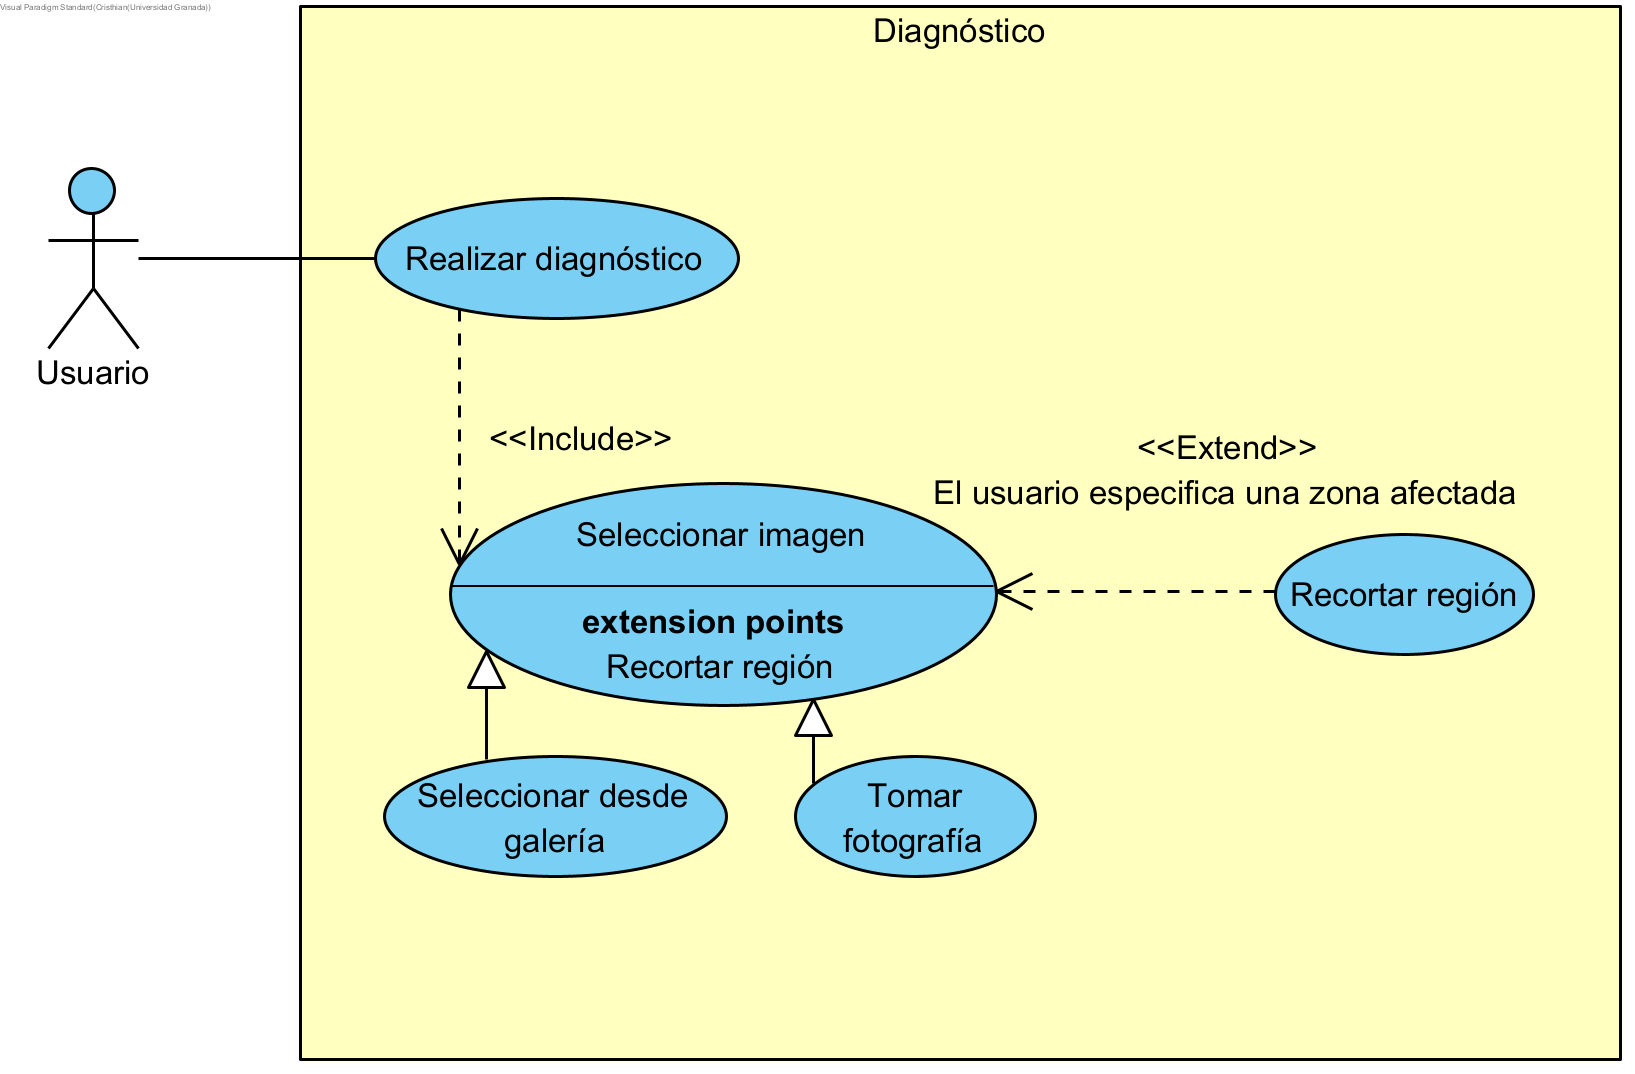
\includegraphics[scale = 0.9]{imagenes/TomarFoto.png}
 	\caption{Caso de uso: Diagnóstico}
 	\label{fig:diagcu}
 \end{figure}
 
 
  \begin{figure}[H]
 	\centering
 	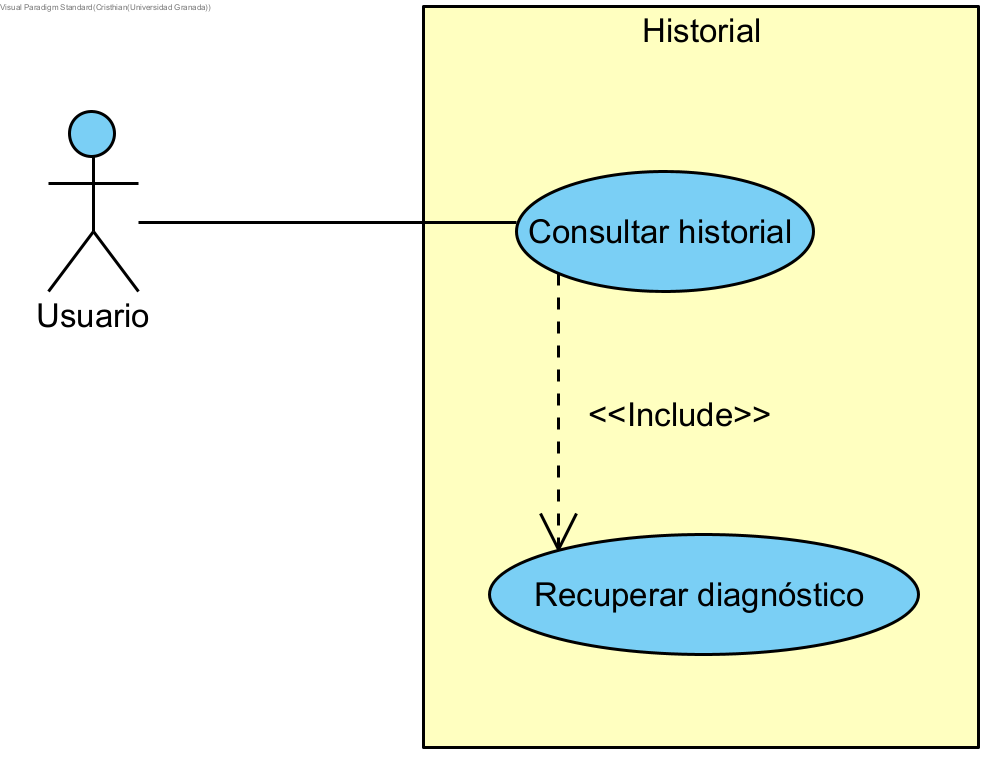
\includegraphics[scale = 1]{imagenes/Historial.png}
 	\caption{Caso de uso: Consulta de historial}
 	\label{fig:histcu}
 \end{figure}

Si agrupamos las funcionalidades en paquetes, podemos obtener un modelo visual que organiza los contenidos de los casos de uso en lo que  será la estructura del proyecto. El resultado es un diagrama bastante simple, contenido en la figura \ref{fig:paquetes}.

\begin{figure}[H]
	\centering
	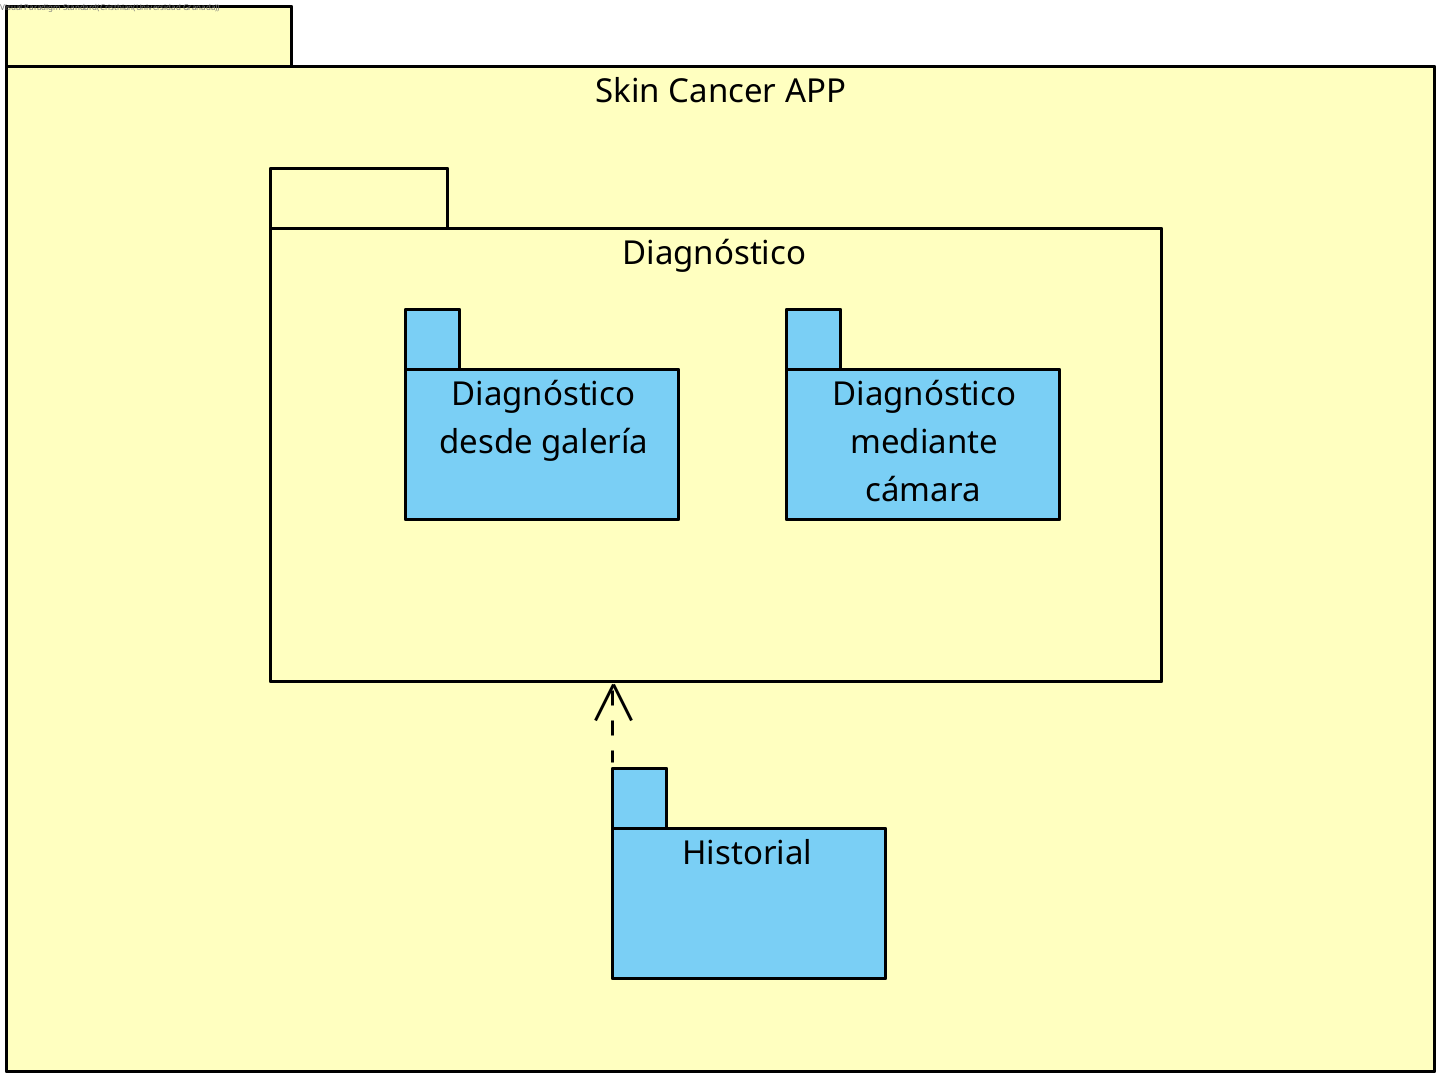
\includegraphics[scale = 0.7]{imagenes/DiagramaPaquetes.png}
	\caption{Diagrama de paquetes}
	\label{fig:paquetes}
\end{figure}

\subsection{Actores}

En el sistema que estamos diseñando, únicamente disponemos de un actor presente: el usuario, paciente de una enfermedad cutánea, que desea emplear el sistema para conocer qué enfermedad sufre en su piel. Se trata de una interacción directa con la aplicación, donde no intervienen otros actores humanos. En la tabla \ref{fig:actorusuario}, podemos apreciar una descripción detallada de sus características.

  \begin{table}[H]
	\centering
	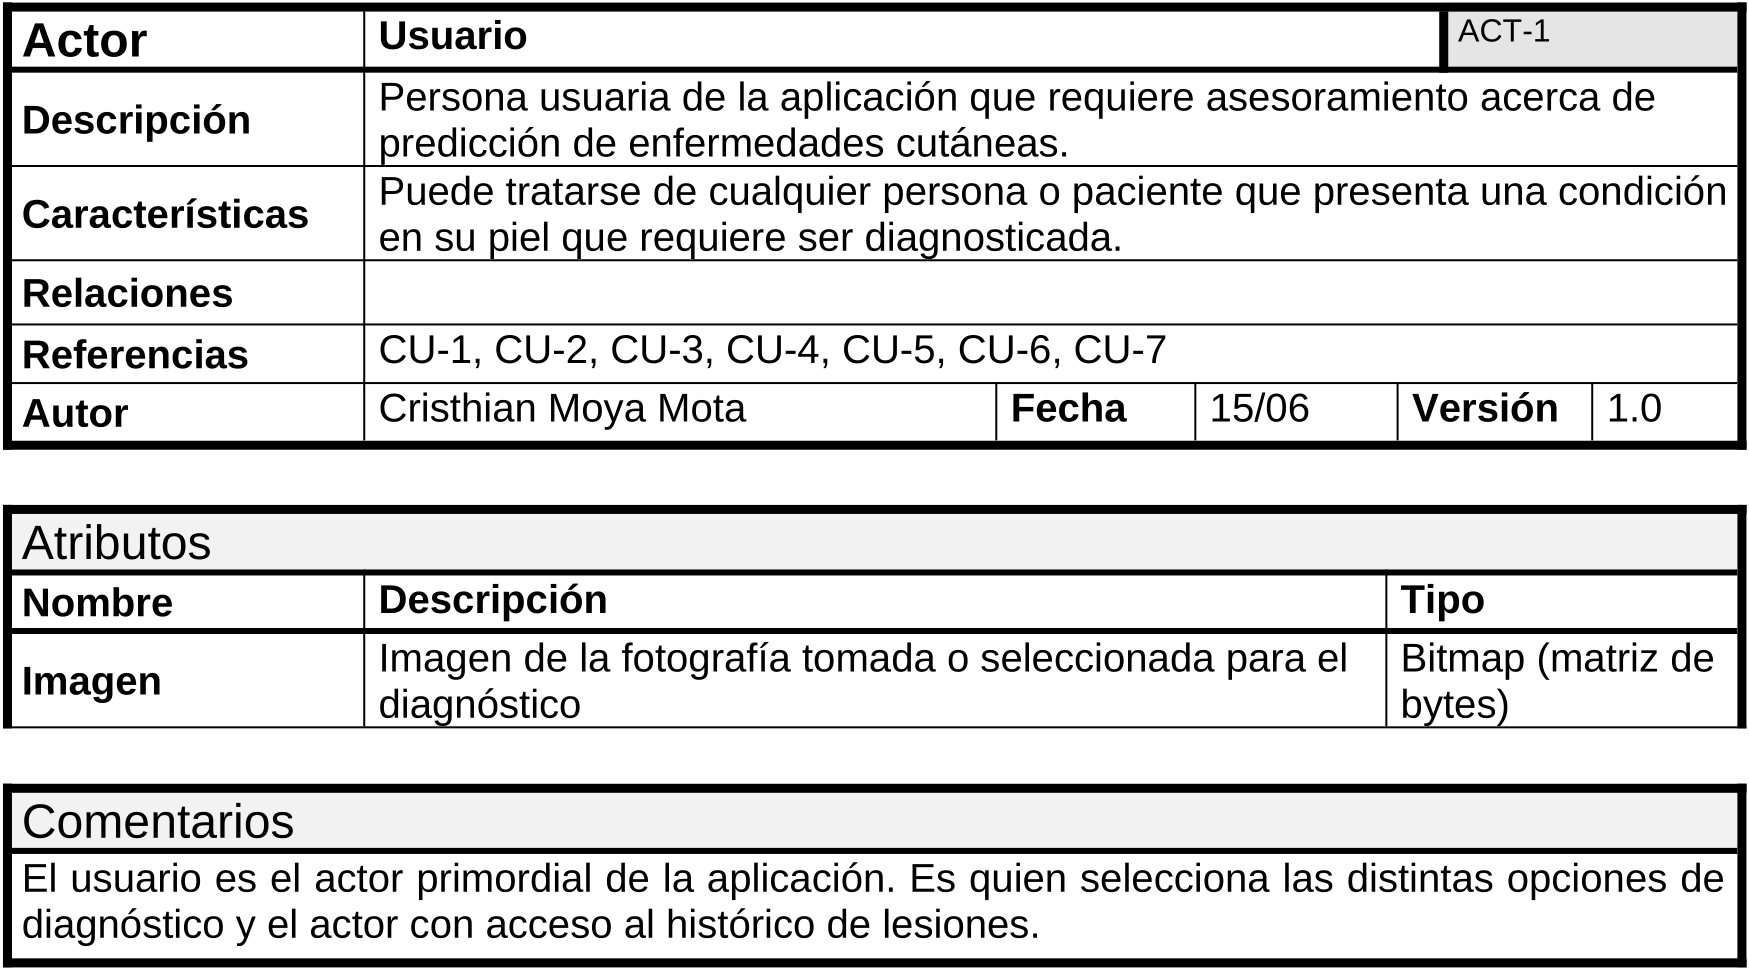
\includegraphics[scale = 0.2]{imagenes/tablausuario.png}
	\caption{Actor: usuario}
	\label{fig:actorusuario}
\end{table}

\subsection	{Descripción extendida de los casos de uso}

Para comprender adecuadamente las implicaciones de cada caso de uso, debemos de realizar un análisis en detalle del mismo. En las tablas mostradas a continuación, podemos observar numerados, los 7 casos identificables: \textit{CU-1} (tabla \ref{fig:cu1}), \textit{CU-2} (tabla \ref{fig:cu2}), \textit{CU-3} (tabla \ref{fig:cu3}), \textit{CU-4} (tabla \ref{fig:cu4}), \textit{CU-5} (tabla \ref{fig:cu5}), \textit{CU-6} (tabla \ref{fig:cu6}) y \textit{CU-7} (tabla \ref{fig:cu7}).

  \begin{table}[H]
	\centering
	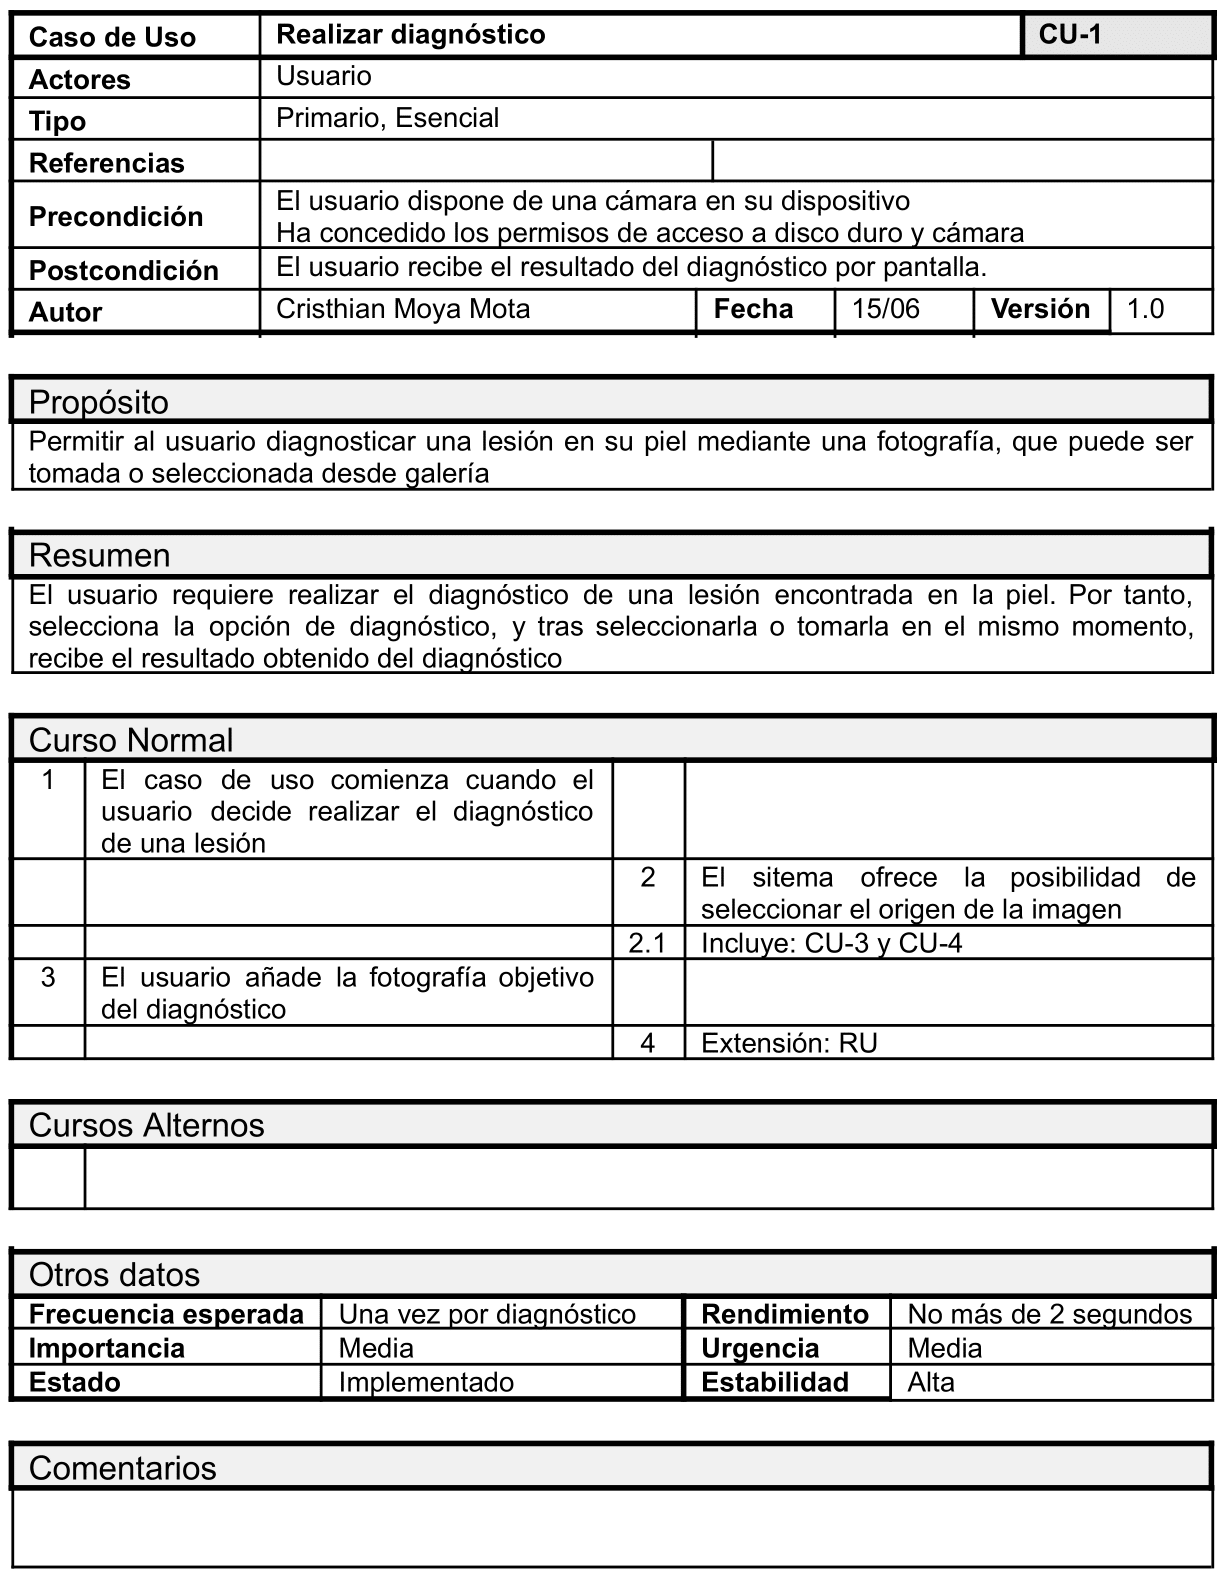
\includegraphics[scale=0.81]{imagenes/cu-1.png}
	\caption{Caso de uso CU-1: realizar diagnóstico}
	\label{fig:cu1}
\end{table}


  \begin{table}[H]
	\centering
	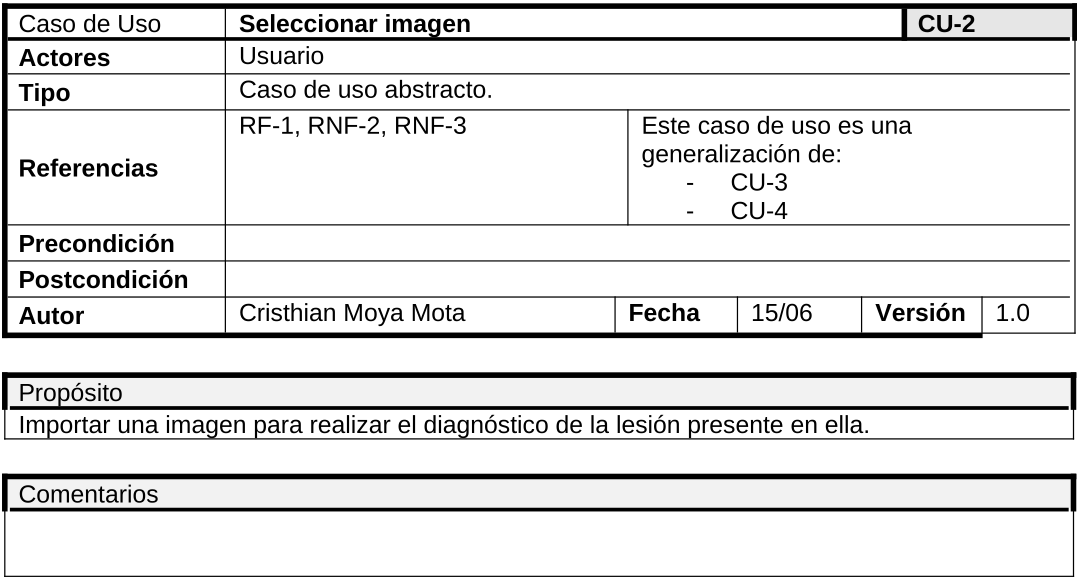
\includegraphics[scale=0.85]{imagenes/cu-2.png}
	\caption{Caso de uso CU-2: seleccionar imagen}
	\label{fig:cu2}
\end{table}

  \begin{table}[H]
	\centering
	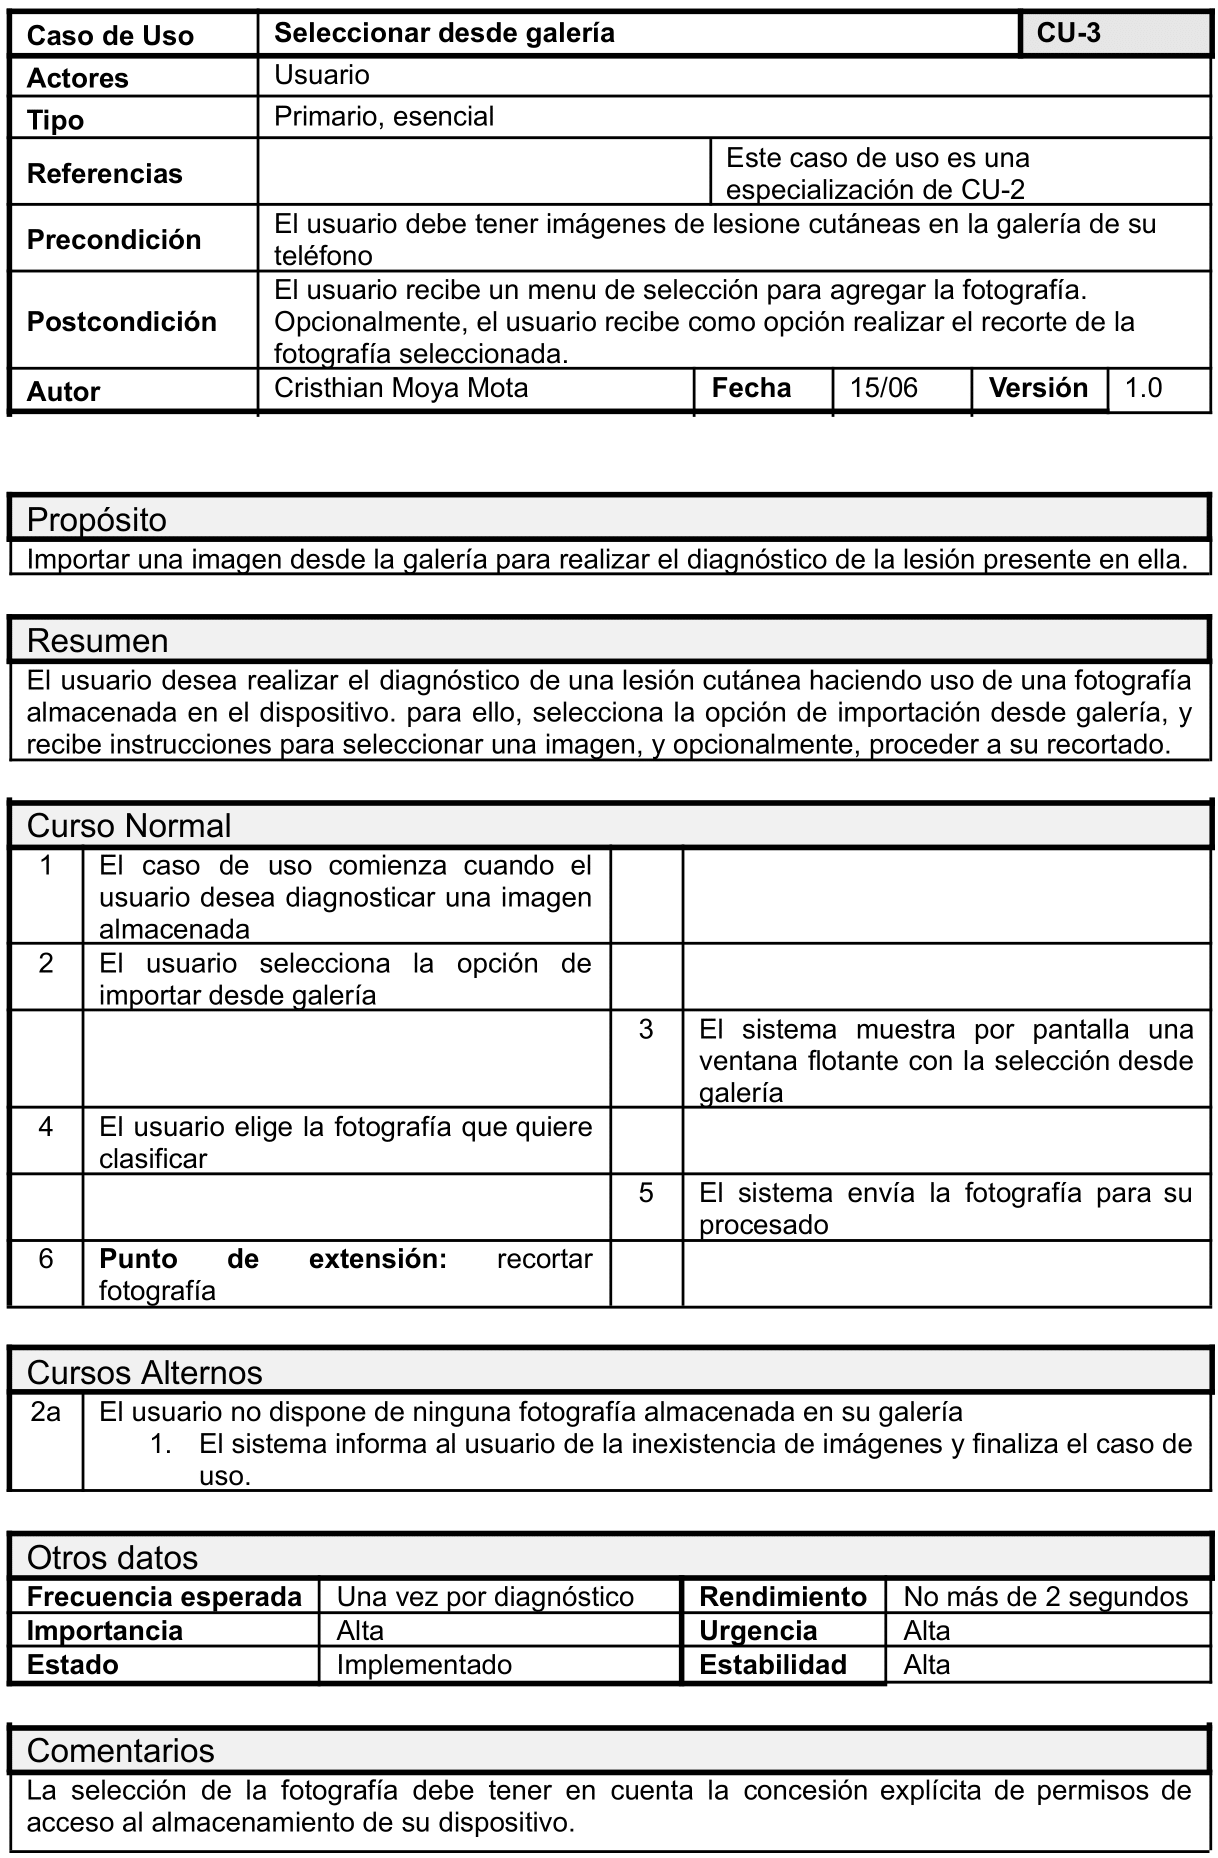
\includegraphics[scale=0.85]{imagenes/cu-3.png}
	\caption{Caso de uso CU-3: seleccionar desde galería}
	\label{fig:cu3}
\end{table}

  \begin{table}[H]
	\centering
	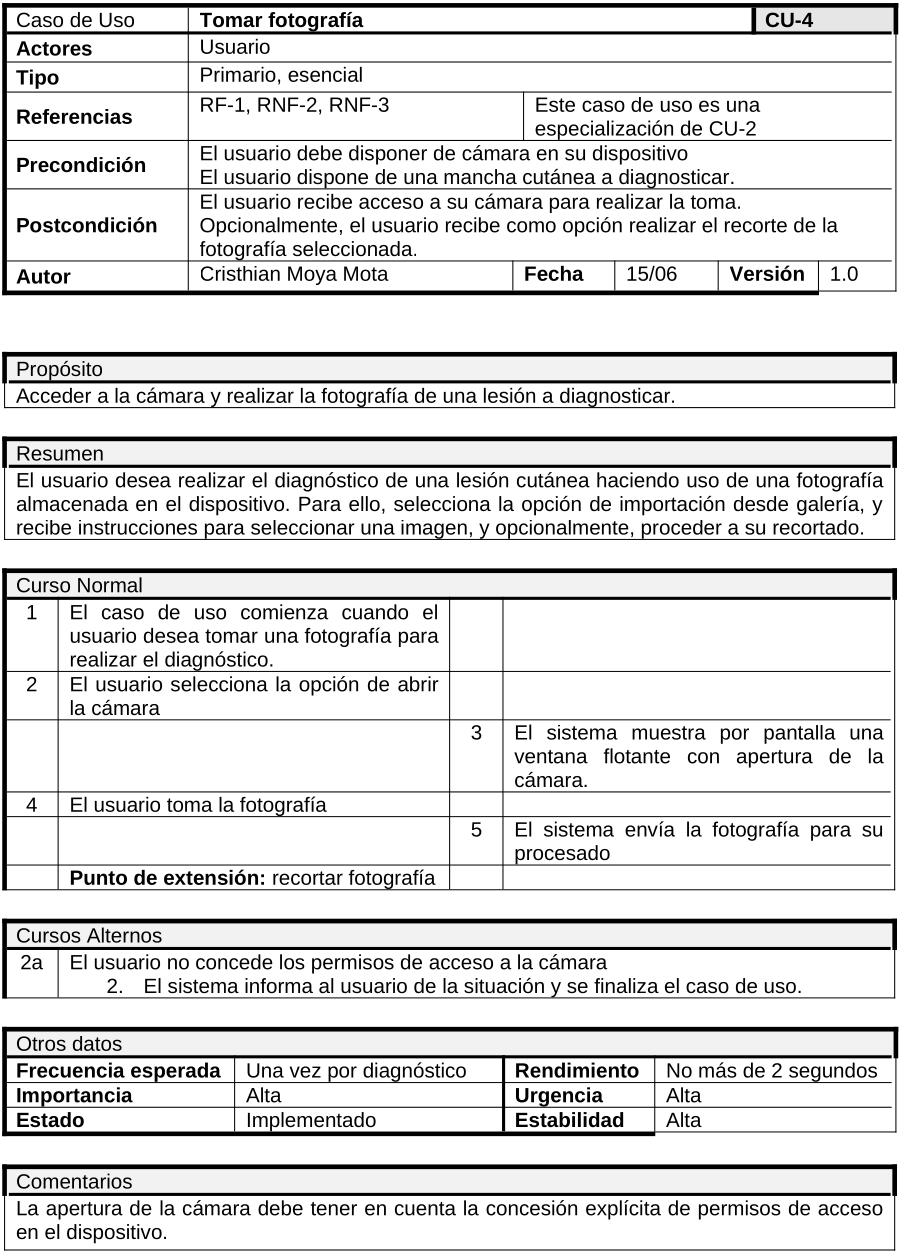
\includegraphics[scale=0.85]{imagenes/cu-4.png}
	\caption{Caso de uso CU-4: tomar fotografía}
	\label{fig:cu4}
\end{table}

  \begin{table}[H]
	\centering
	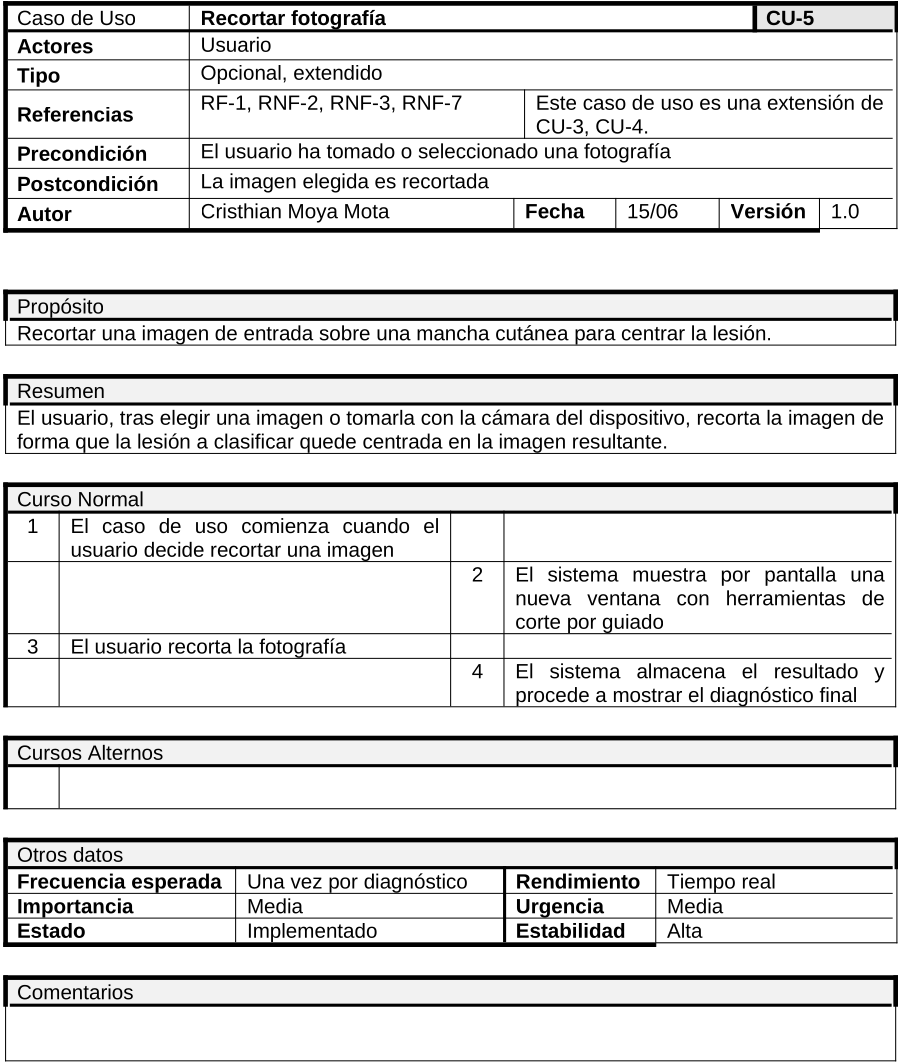
\includegraphics[scale=0.85]{imagenes/cu-5.png}
	\caption{Caso de uso CU-5: recortar región}
	\label{fig:cu5}
\end{table}

\begin{table}[H]
	\centering
	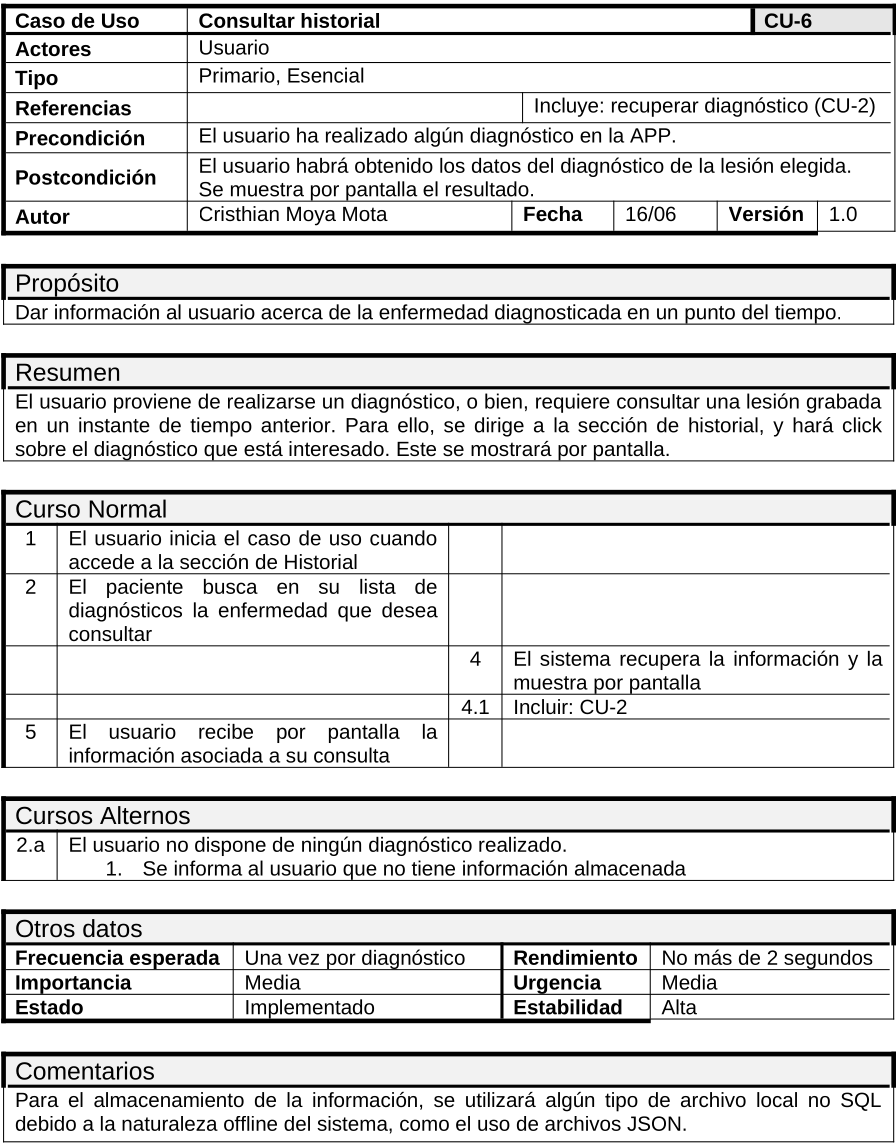
\includegraphics[scale=0.85]{imagenes/cu-6.png}
	\caption{Caso de uso CU-6: consultar historial}
	\label{fig:cu6}
\end{table}

\begin{table}[H]
	\centering
	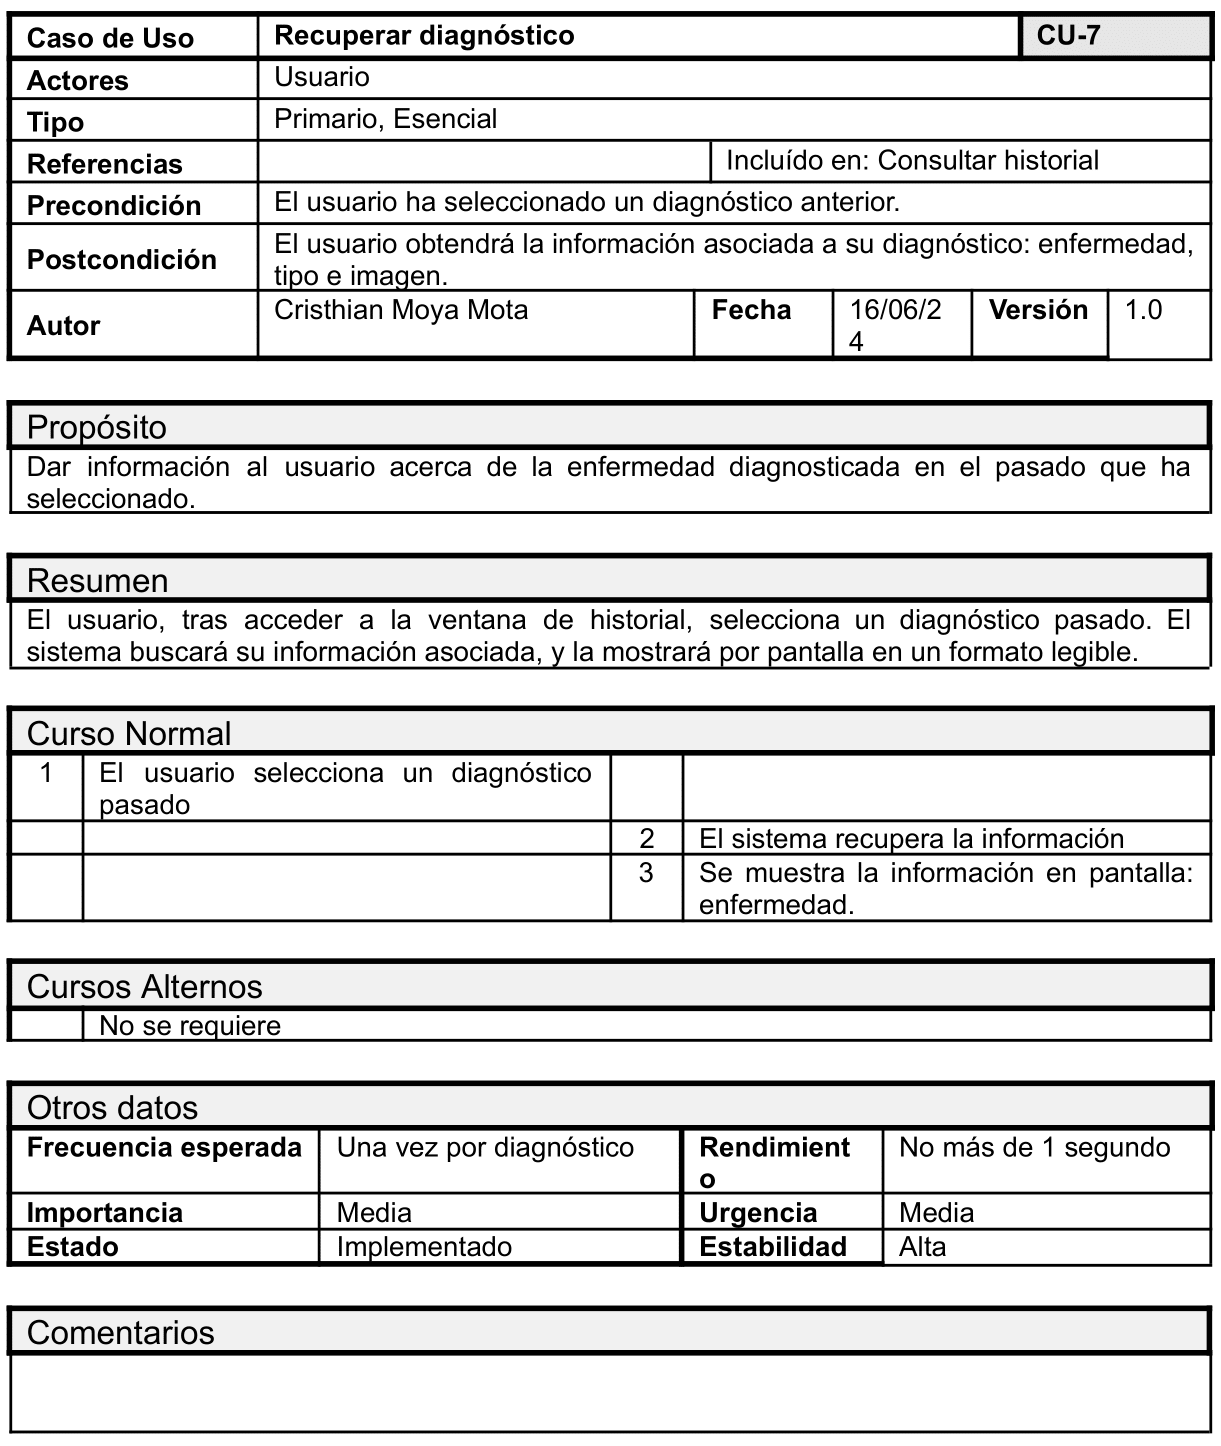
\includegraphics[scale=0.85]{imagenes/cu-7.png}
	\caption{Caso de uso CU-7: recuperar diagnóstico}
	\label{fig:cu7}
\end{table}

De esta forma, ya disponemos de las interacciones detalladas que existen entre cada uno de los casos de uso, y podemos elaborar el diagrama de concepto asociado que nos describe la cardinalidad de las mismas. Dicho diagrama, se convertirá posteriormente en la base para la creación del diagrama de clases de diseño.

\section{Modelo de análisis}
Una vez hemos descrito adecuadamente los casos de uso obtenidos, podemos pasar a la fase de análisis del problema. En esta fase, una vez se han detectado todos los requisitos, procedemos a representarlos formalmente mediante modelos. Concretamente, tenemos dos tipos de modelos: estático y dinámico.

\begin{enumerate}
	\item \textbf{Modelo estático}.  Muestra la estructura que sigue el proyecto, a través de un modelo conceptual, donde se relacionan las distintas entidades detectadas en el problema. Se representa a través de un diagrama conceptual.
	\item \textbf{Modelo dinámico}. Representa las relaciones que se producen durante el uso del proyecto, es decir, representan el comportamiento del mismo. Se hace uso de los diagramas de secuencia y los contratos de diseño.
\end{enumerate} 

Comenzaremos por la especificación del diagrama conceptual, y posteriormente al comportamiento dinámico del sistema.

\subsection{Modelo estático: diagrama conceptual}

Para la especificación del modelo estático, debemos realizar una análisis de los conceptos que componen el sistema, e identificar aquellos que verdaderamente participan en él. De esta forma, podemos construir el diagrama de conceptual, y representar de manera estática la estructura del proyecto.

Atendiendo a los objetivos especificados en el capítulo \ref{cap:objetivos} y la descripción del problema que extendimos en el apartado \ref{sec:descripcion}, podemos identificar los siguientes conceptos clave:

\begin{itemize}
	\item \textbf{Imagen}: elemento clave del sistema, sobre el cual se realiza la clasificación de la enfermedad.  A su vez, podemos encontrar dos tipos muy similares, pero con distintos tipos de almacenaje: \textbf{ImagenDisco} e \textbf{ImagenCámara}, siendo la primera obtenida a partir de su dirección URI (identificador de recursos uniforme, i.e, una dirección única), y la segunda, directamente como mapa de bits procedente de la cámara.
	\item  \textbf{Patología} (llamada como \textbf{InfoPatología}): se trata de la información asociada a la enfermedad que el usuario recibe como descripción.
	\item \textbf{Diagnóstico} (llamado como \textbf{DiagnósticoData}). Información completa, que incluye la descripción de la patología, y la imagen asociada, cuyo objetivo es ser almacenado en el historial para ser recuperado cuando se desee.
	\item \textbf{Historial} Estructura de información que puede contener ninguno o varios diagnósticos previamente realizados de forma que el usuario pueda consultar la evolución de su enfermedad, o buscar antiguas prognosis.
\end{itemize}

De esta forma, nos queda el diagrama conceptual apreciable en la figura \ref{fig:conceptual}.

\begin{figure}[H]
	\centering
	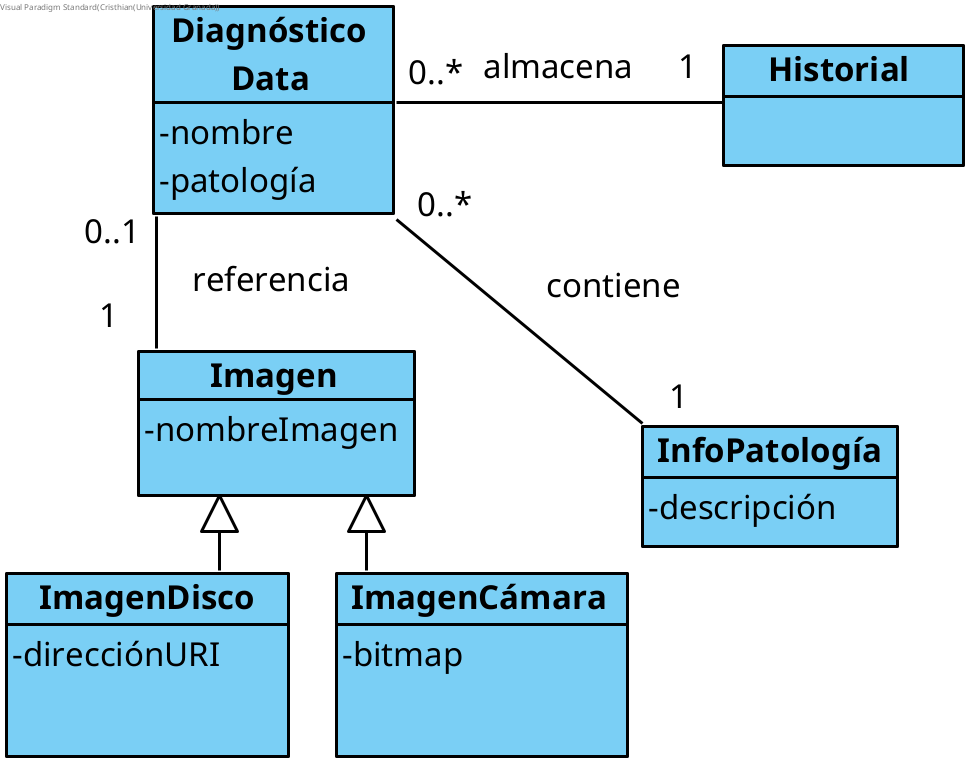
\includegraphics[scale = 1.2]{imagenes/MapaConceptual.png}
	\caption{Diagrama conceptual}
	\label{fig:conceptual}
\end{figure}

\subsection{Modelo dinámico: diagramas de secuencia y contratos}

En esta sección, estudiaremos las interacciones entre las diferentes partes del sistema. Para ello, emplearemos los diagramas de secuencia y los contratos de C. Larman \cite{larman2003uml}.

\subsubsection{Diagrama de secuencia}
En un diagrama de secuencia, se muestran como los eventos que generan los actores del sistema provocan la ejecución de una operación por el Sistema, siendo visto este como una caja negra. En nuestro caso, las acciones son bastante limitadas, ya que únicamente disponemos de un actor: el usuario de la aplicación. 

Partiendo de las acciones definidas en los casos de uso, junto con los posibles parámetros de entrada que puede requerir cada evento producido. En este caso, además, se ha empleado el uso de un diagrama de secuencia por cada diagrama de casos de uso, de forma que ya quede establecido la separación de funcionalidades.

En la figura \ref{fig:secdiag} podemos apreciar el diagrama de secuencia asociado al diagnóstico, mientras que en la figura \ref{fig:sechistorial}, se represente el diagrama para el subsistema del historial.

\begin{figure}[H]
	\centering
	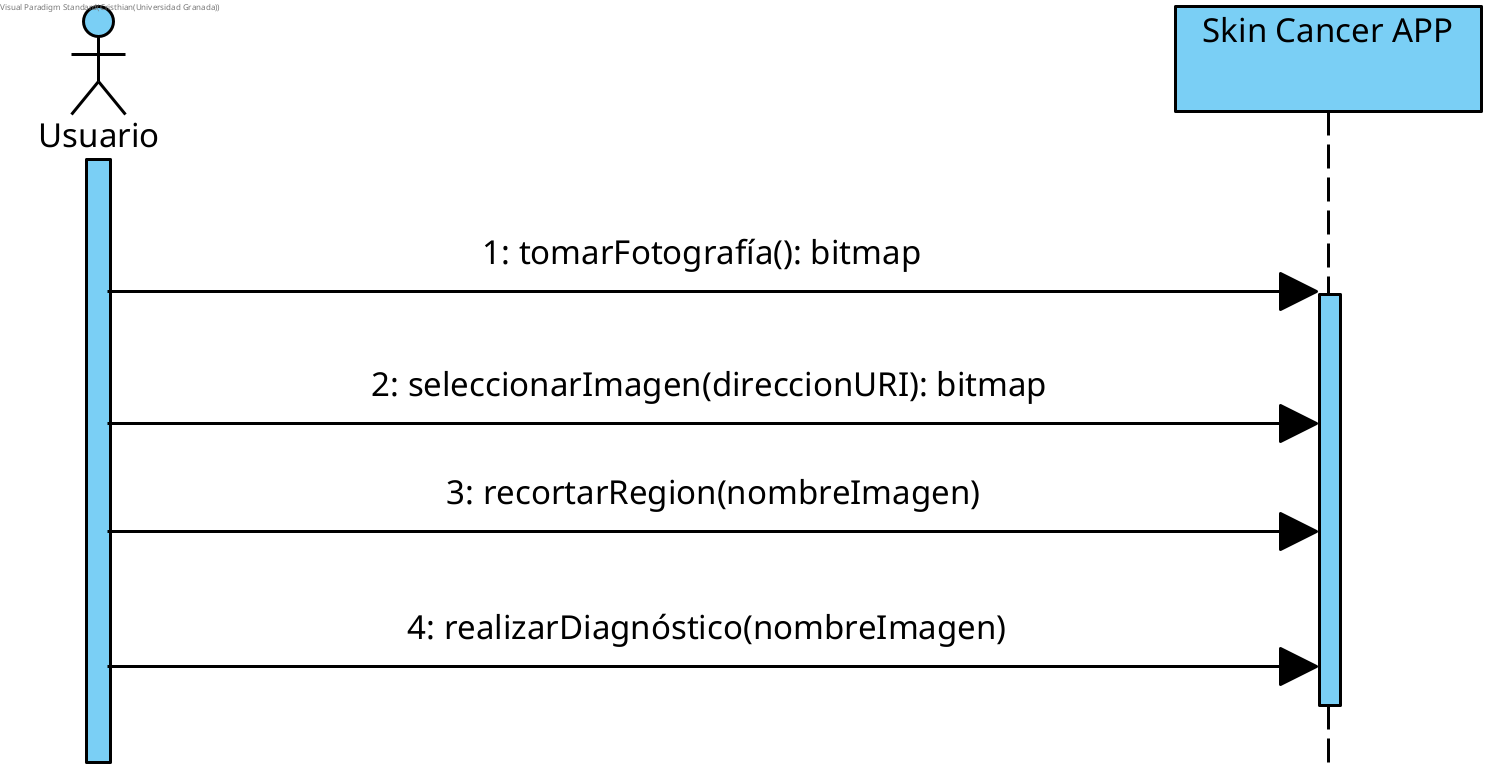
\includegraphics[scale = 1]{imagenes/DiagramaSecuenciaFotografia.png}
	\caption{Diagrama de secuencia para el subsistema de fotografías y diagnóstico.}
	\label{fig:secdiag}
\end{figure}

\begin{figure}[H]
	\centering
	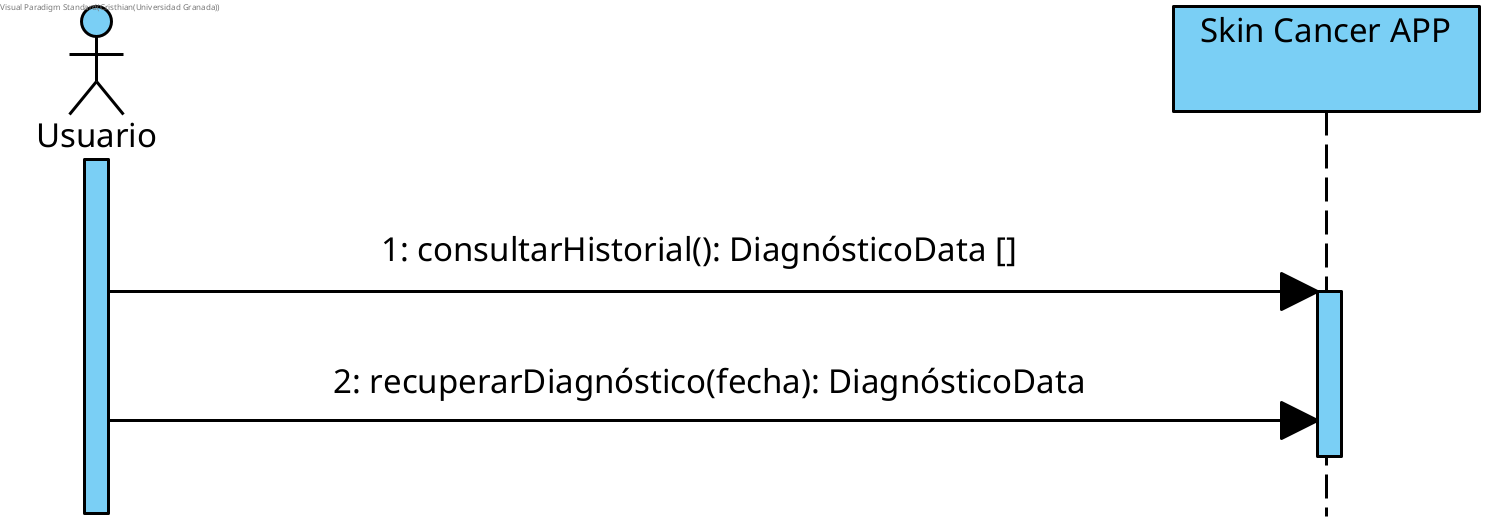
\includegraphics[scale = 1]{imagenes/DiagramaSecuenciaHistorial.png}
	\caption{Diagrama de secuencia para el subsistema de historial.}
	\label{fig:sechistorial}
\end{figure}

 \subsubsection{Contratos}
 
 Una vez queda representado visualmente los eventos que el usuario puede iniciar en el sistema mediante el diagrama de secuencia, debemos	de especificar lo que se desea lograr en cada operación realizada, pero aun sin entrar en detalles de su implementación. No existe un formato estandarizado único como sí lo ha sido hasta ahora el caso de los diagramas UML (Lenguaje unificado de modelado) con los diagramas de caso de uso y los de secuencia. Sin embargo, habitualmente se emplean los contratos de C. Larman \cite{larman2003uml}, donde se presentan las especificaciones de cada operación en un estilo declarativo, y comúnmente estructurado en formato de tabla.
 
 Para cada evento descrito en el modelo de secuencia, obtenemos su correspondiente contrato, que incluirá principalmente las precondiciones, excepciones, descripción de la operación, y postcondiciones que se producen en el sistema.
 
 En este proyecto, obtenemos 6 contratos, representados en las tablas \ref{fig:contrato1}, \ref{fig:contrato2}, \ref{fig:contrato3}, \ref{fig:contrato4},\ref{fig:contrato5} y \ref{fig:contrato6}, siguiendo el orden de los eventos especificados en los diagramas de secuencia \ref{fig:secdiag} y \ref{fig:sechistorial}.
 
 \begin{table}[H]
 	\centering
 	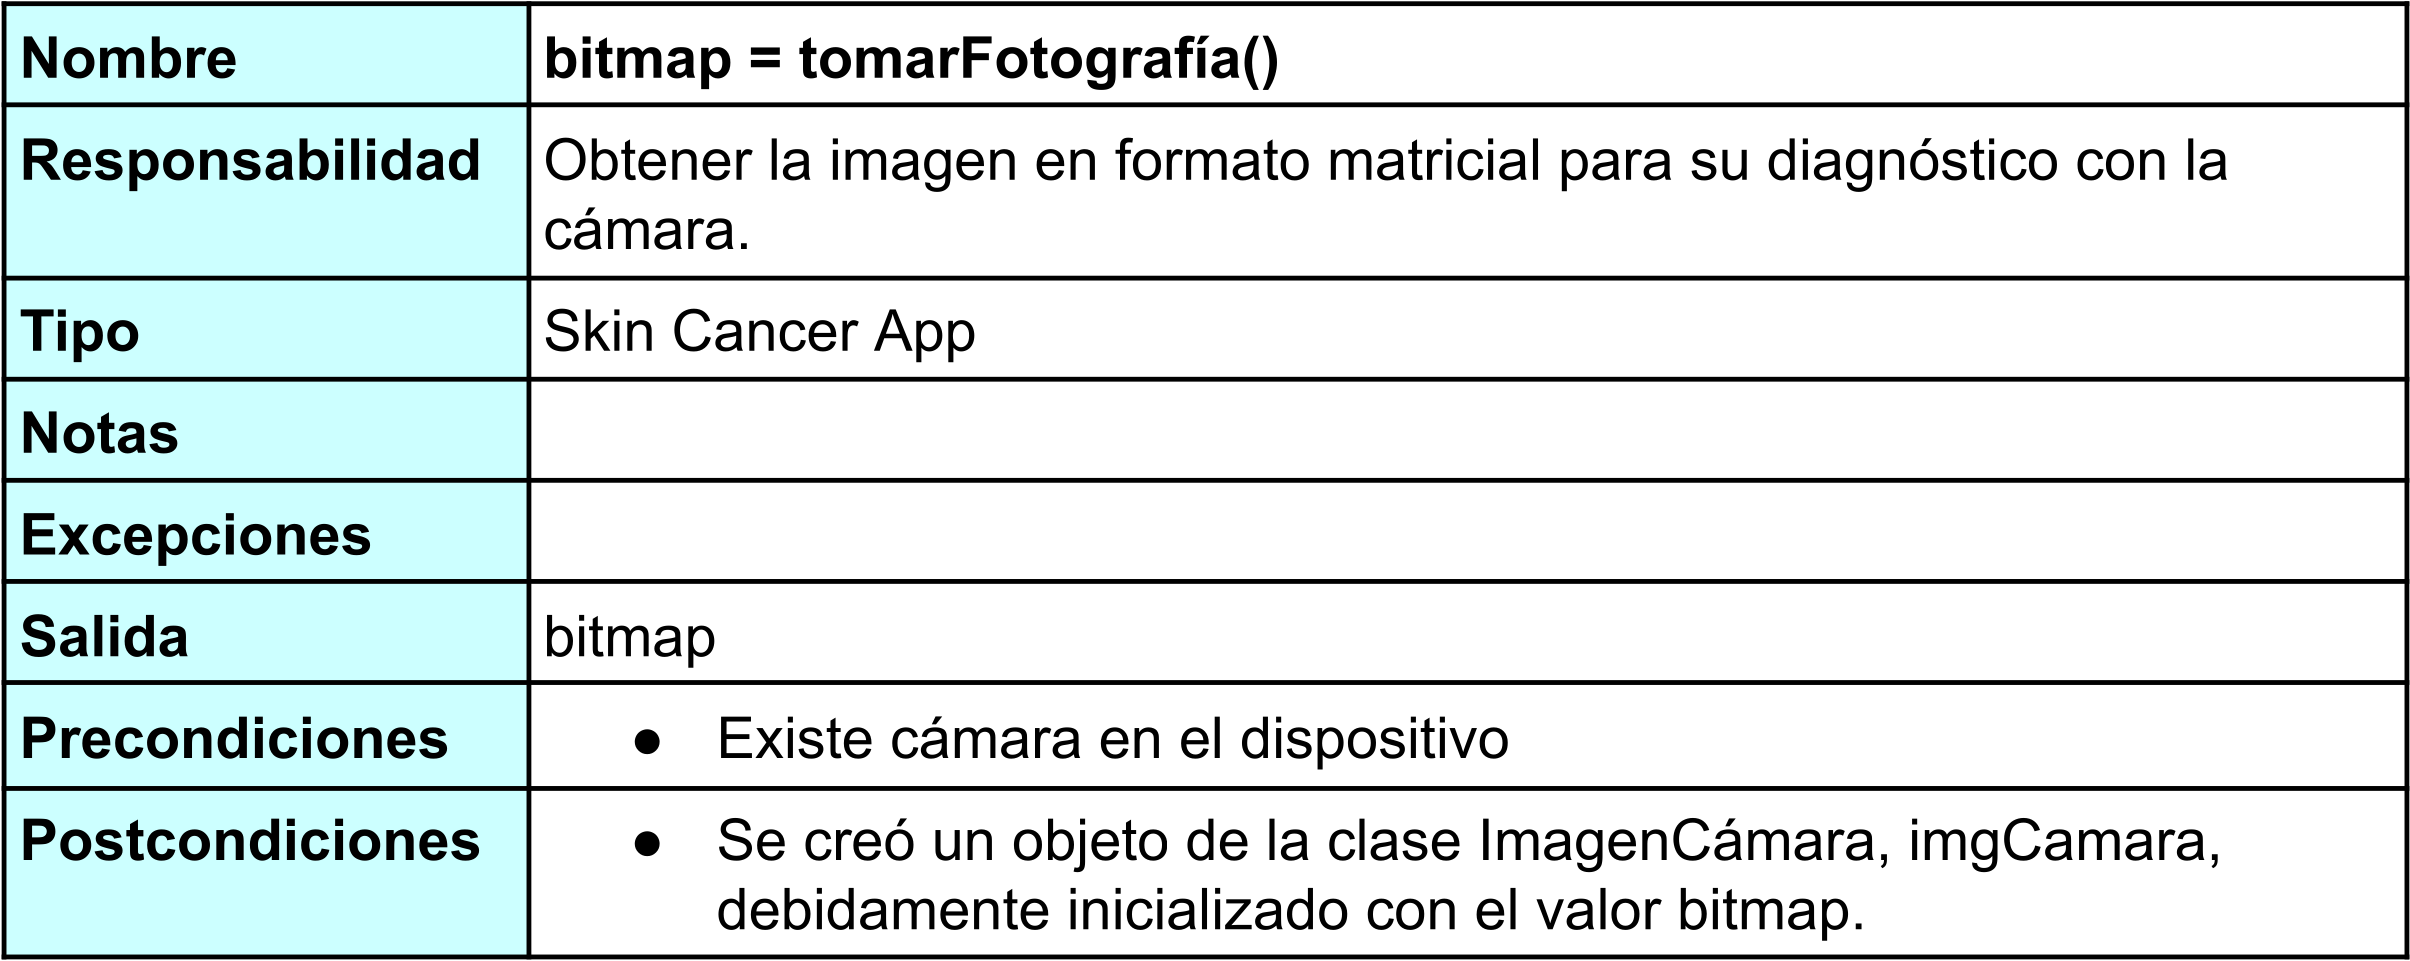
\includegraphics[scale = 0.16]{imagenes/contrato1.png}
 	\caption{Contrato: tomar fotografía.}
 	\label{fig:contrato1}
 \end{table}
 
  \begin{table}[H]
 	\centering
 	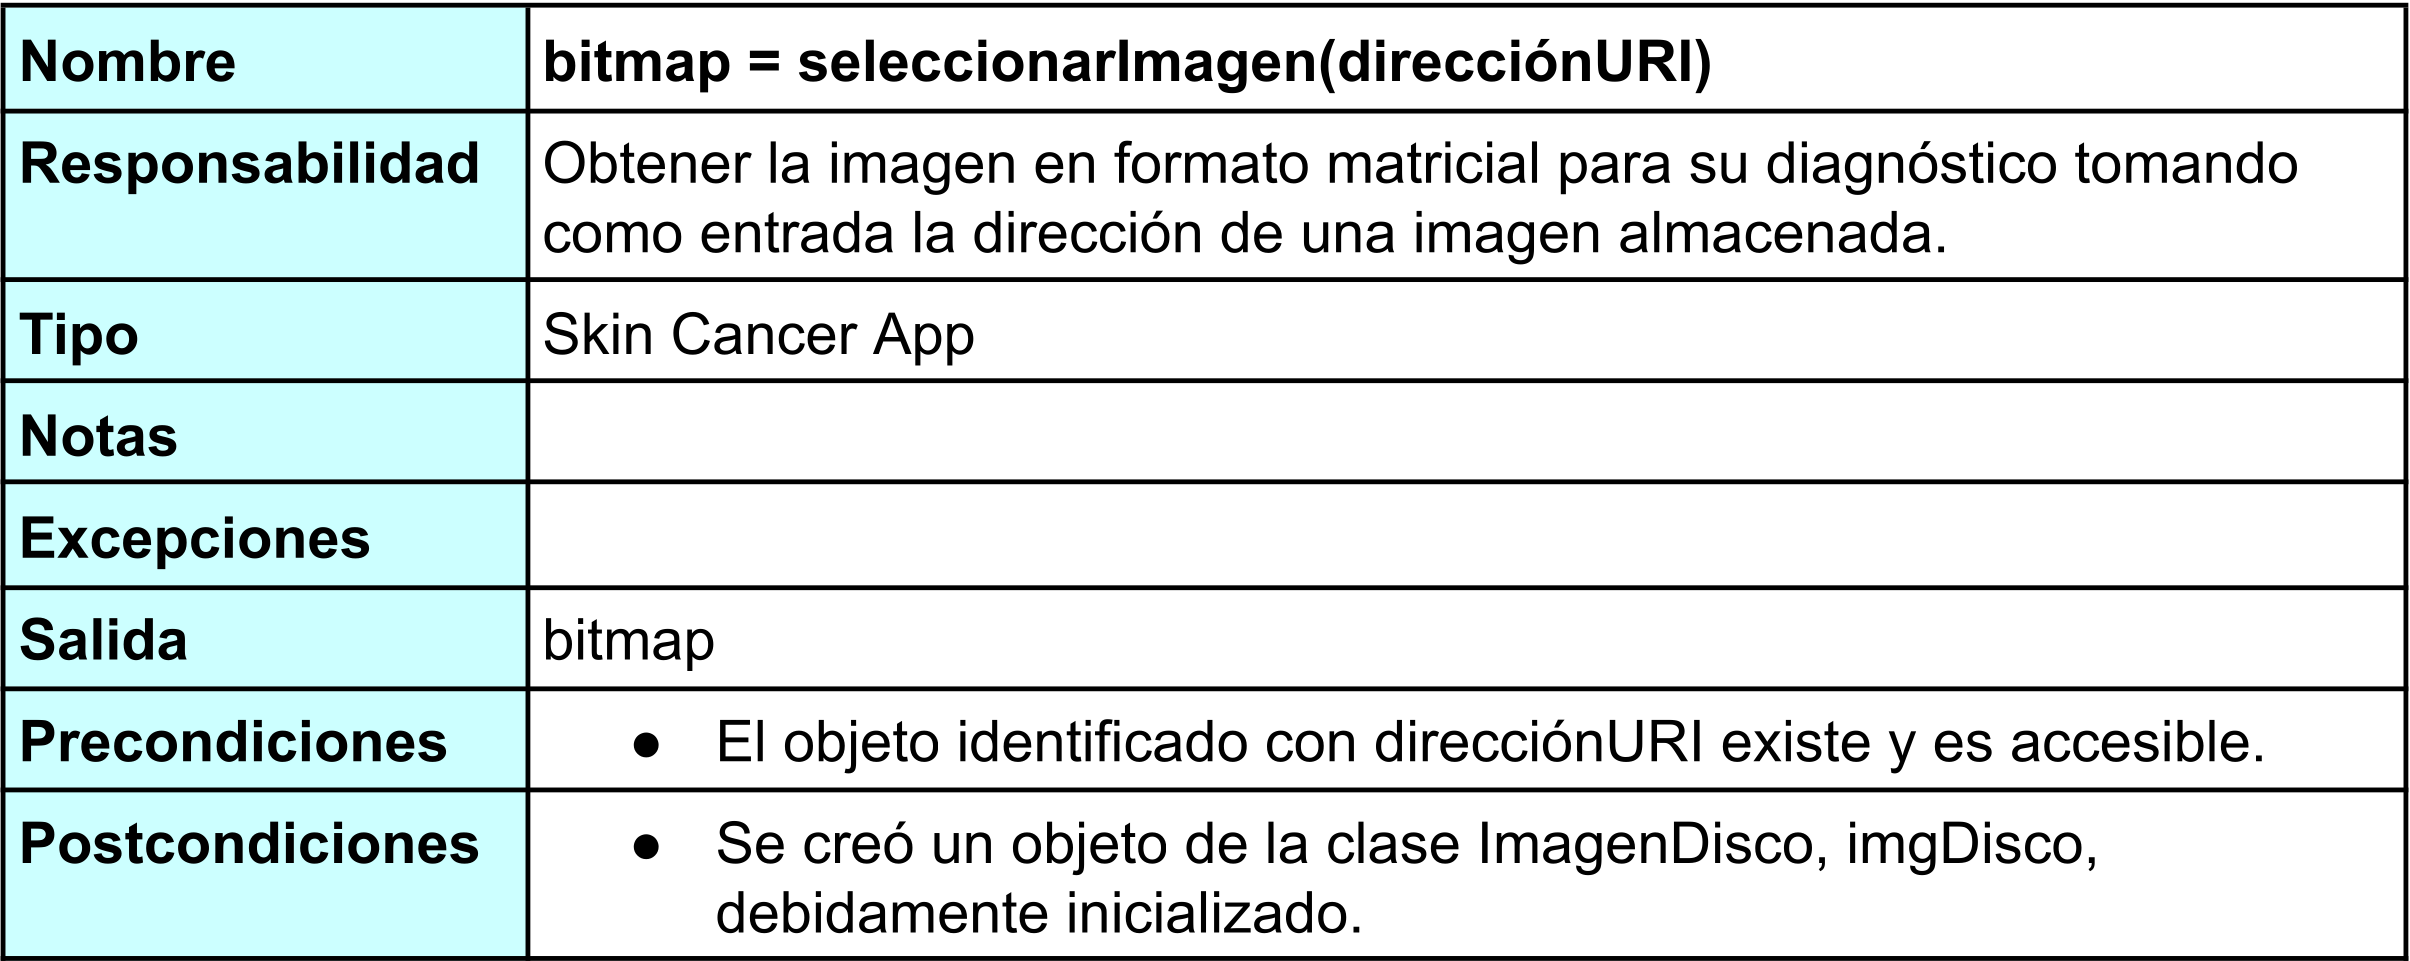
\includegraphics[scale = 0.16]{imagenes/contrato2.png}
 	\caption{Contrato: seleccionar imagen.}
 	\label{fig:contrato2}
 \end{table}
 
   \begin{table}[H]
 	\centering
 	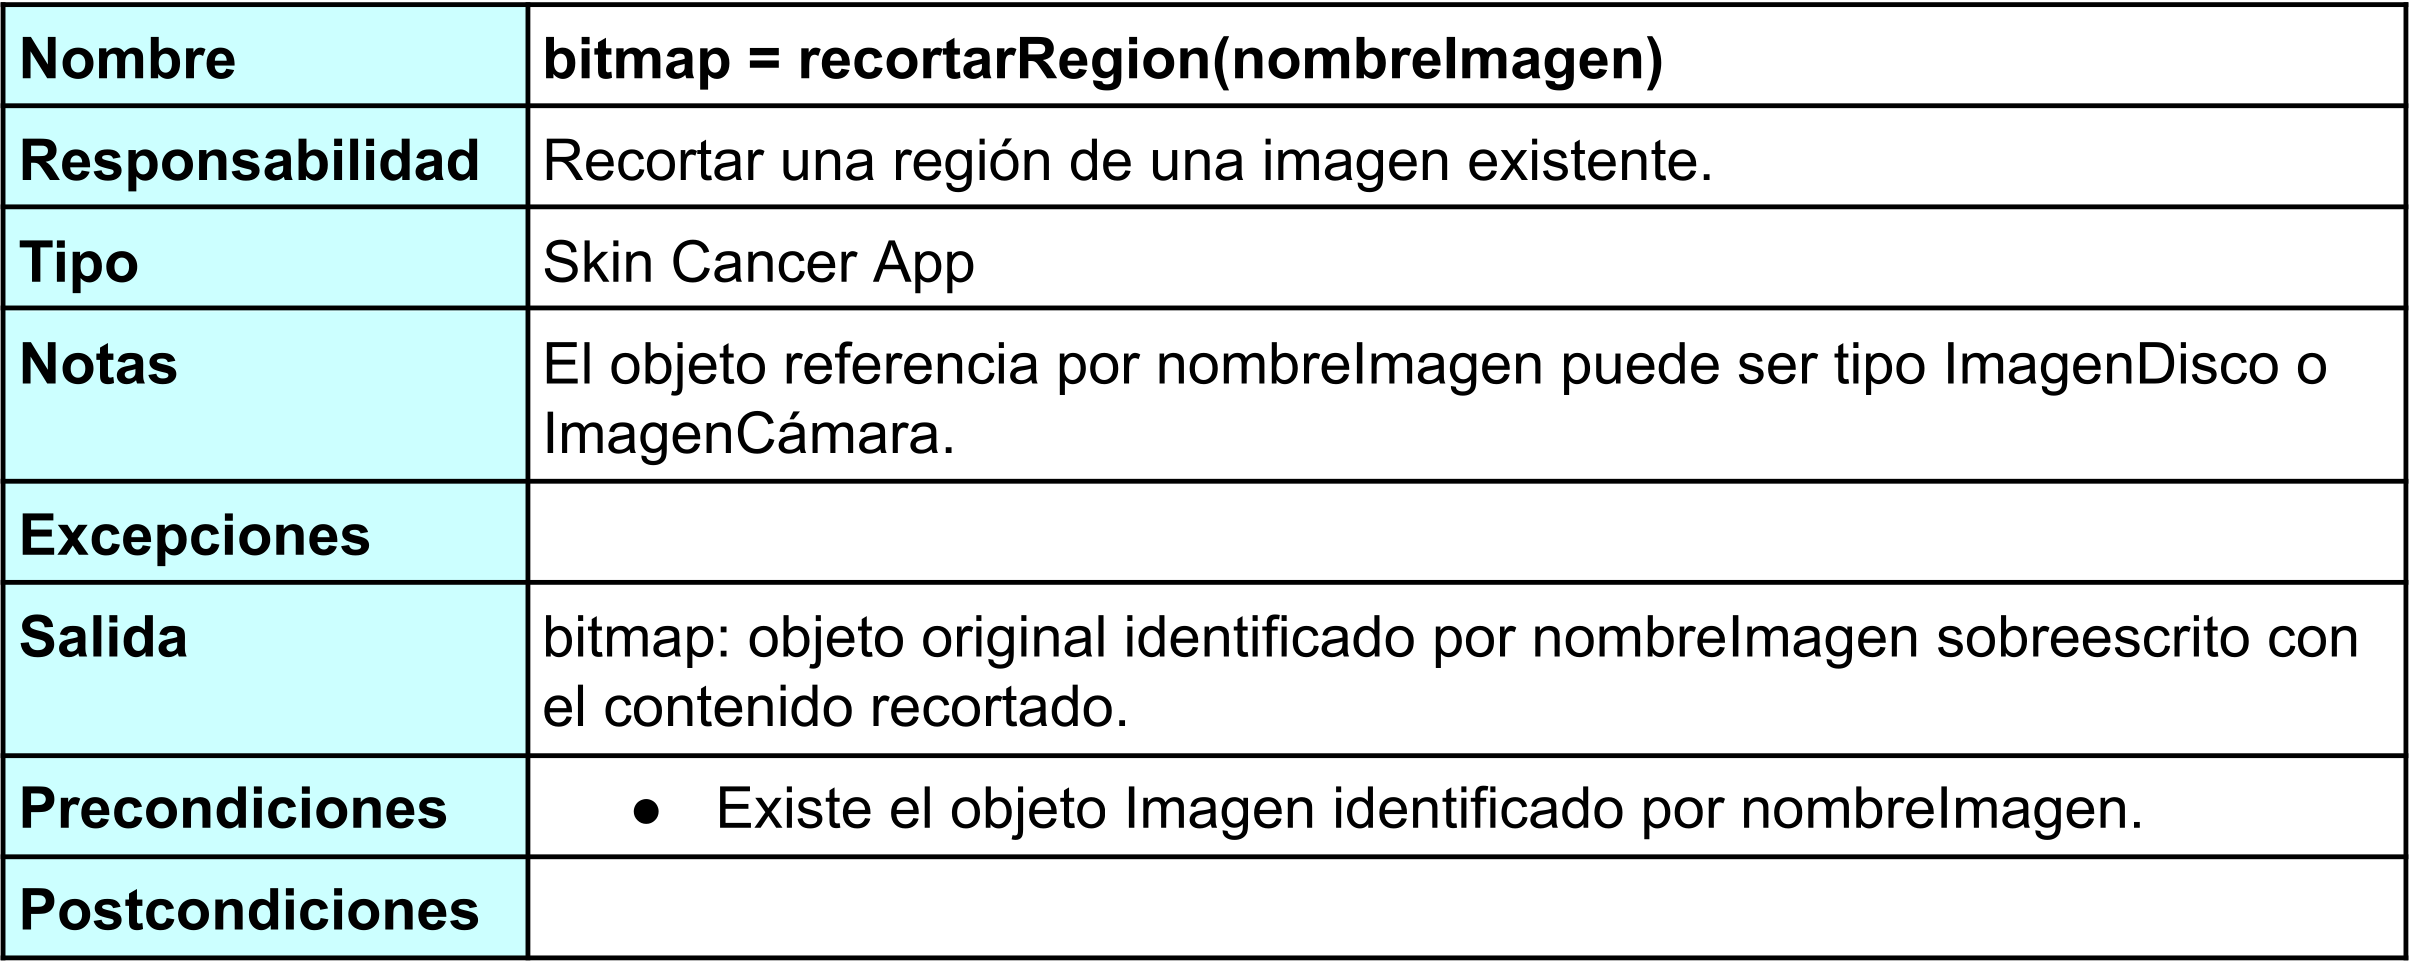
\includegraphics[scale = 0.16]{imagenes/contrato3.png}
 	\caption{Contrato: recortar región de una imagen.}
 	\label{fig:contrato3}
 \end{table}
 
   \begin{table}[H]
 	\centering
 	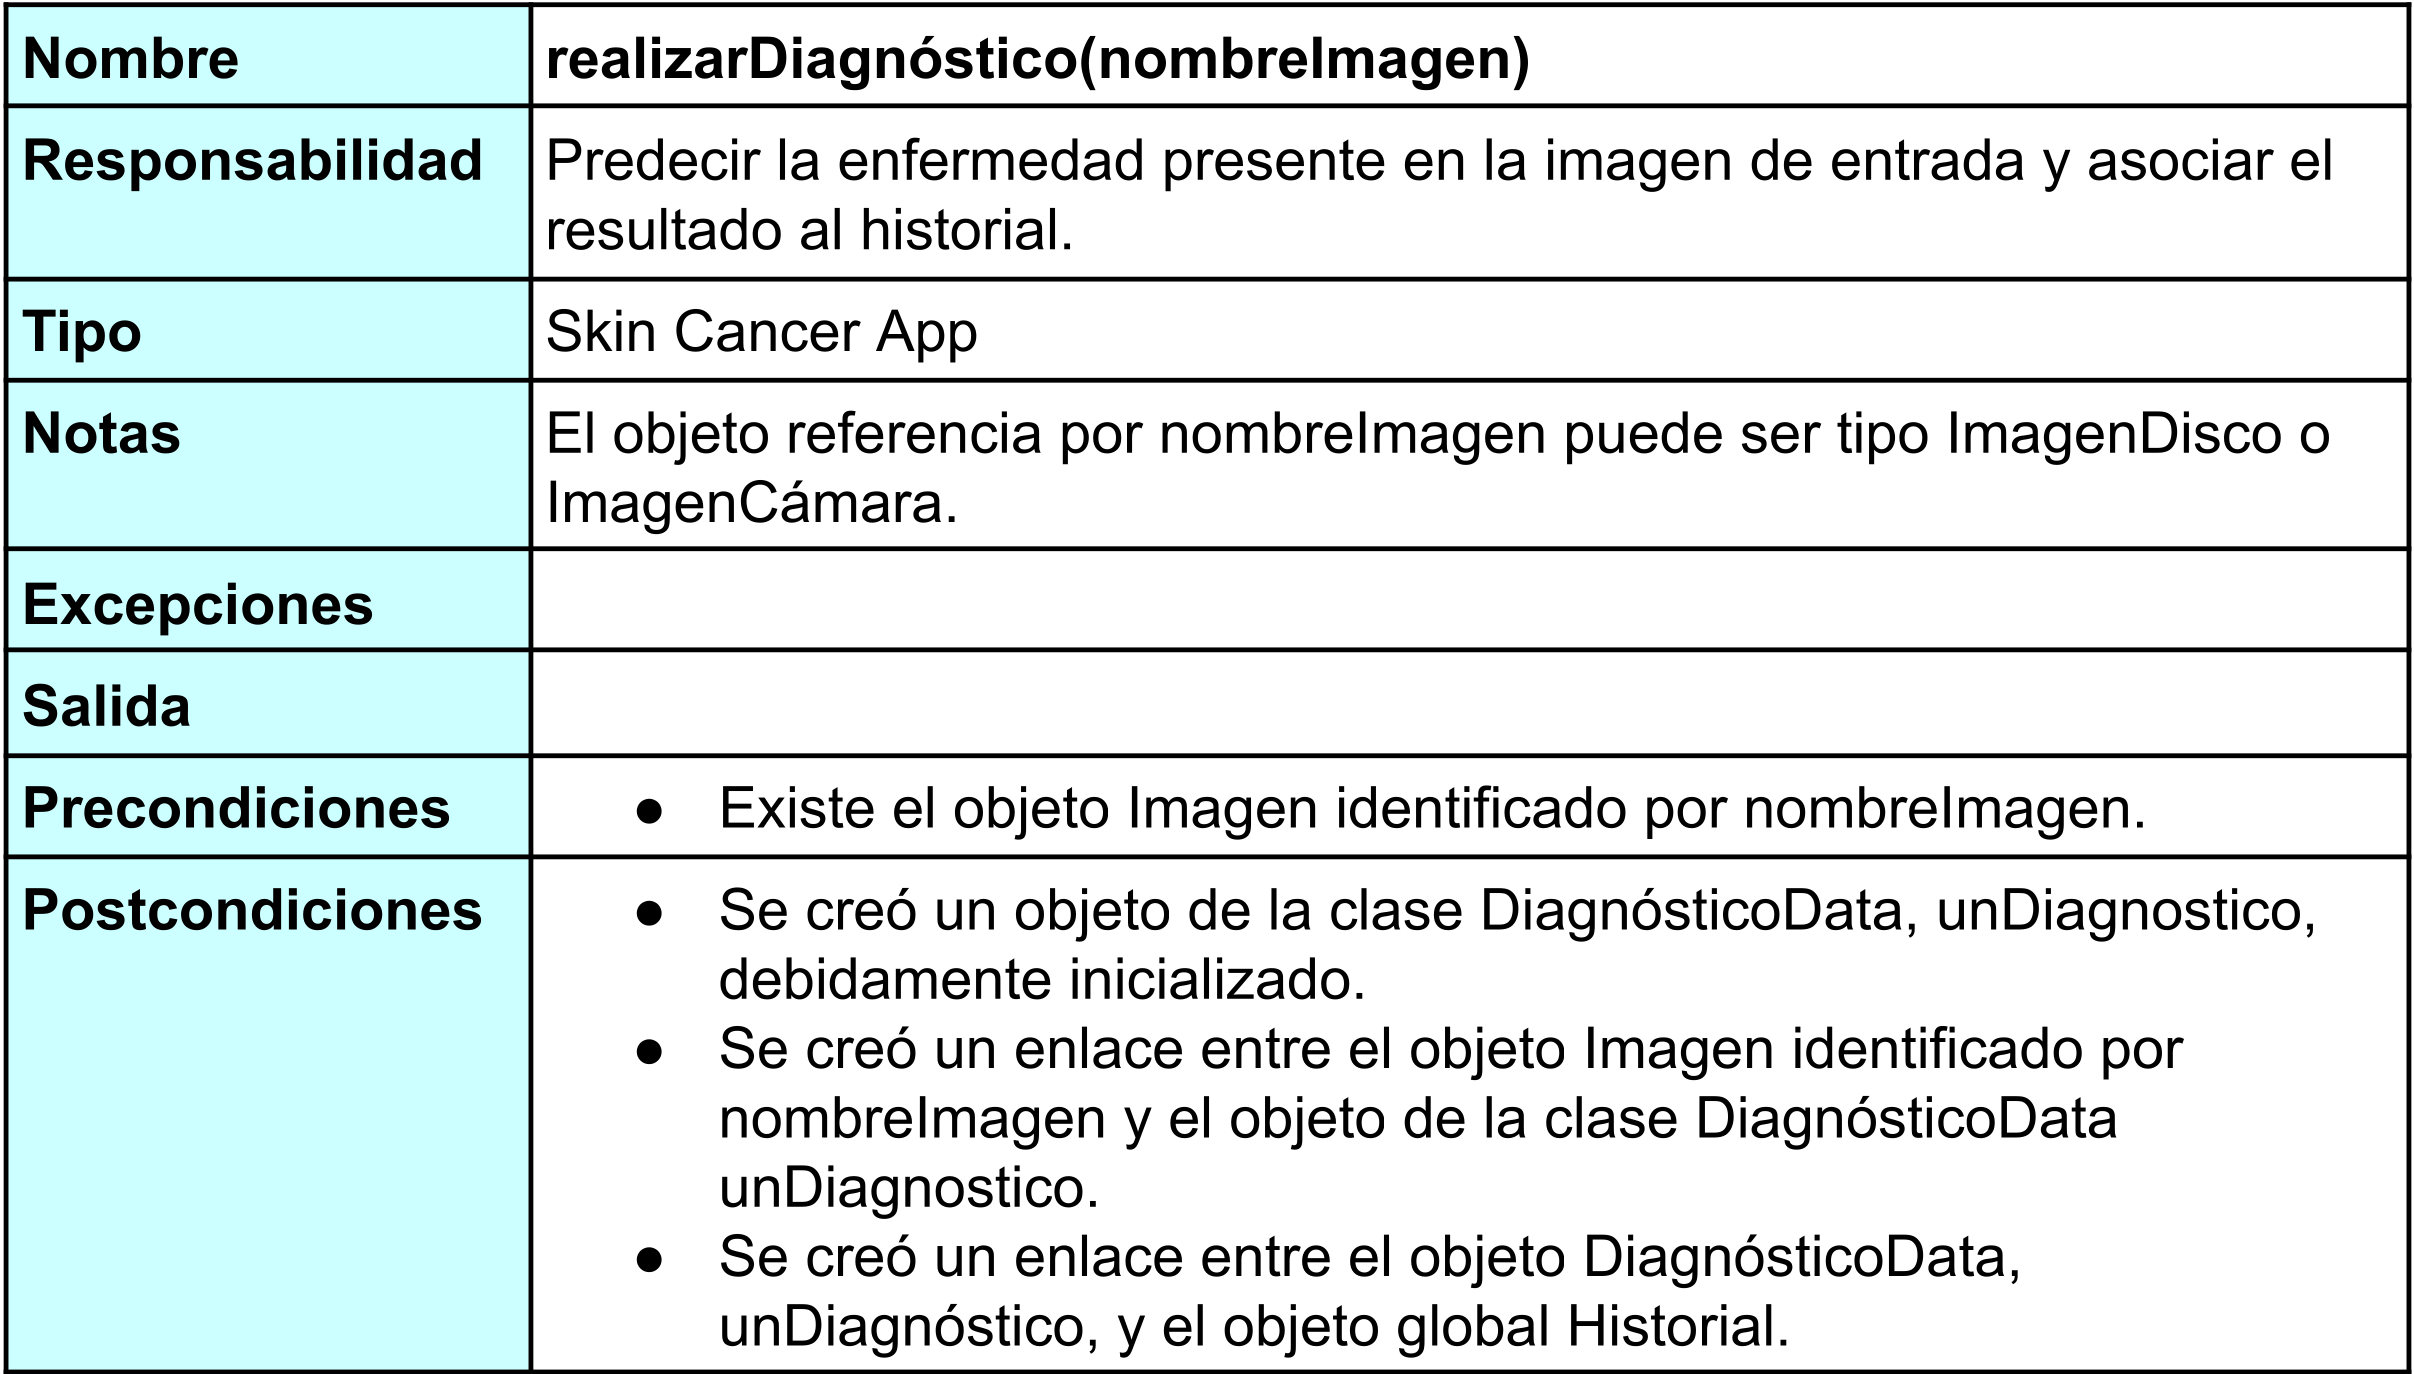
\includegraphics[scale = 0.16]{imagenes/contrato4.png}
 	\caption{Contrato: realizar diagnóstico.}
 	\label{fig:contrato4}
 \end{table}
 
   \begin{table}[H]
 	\centering
 	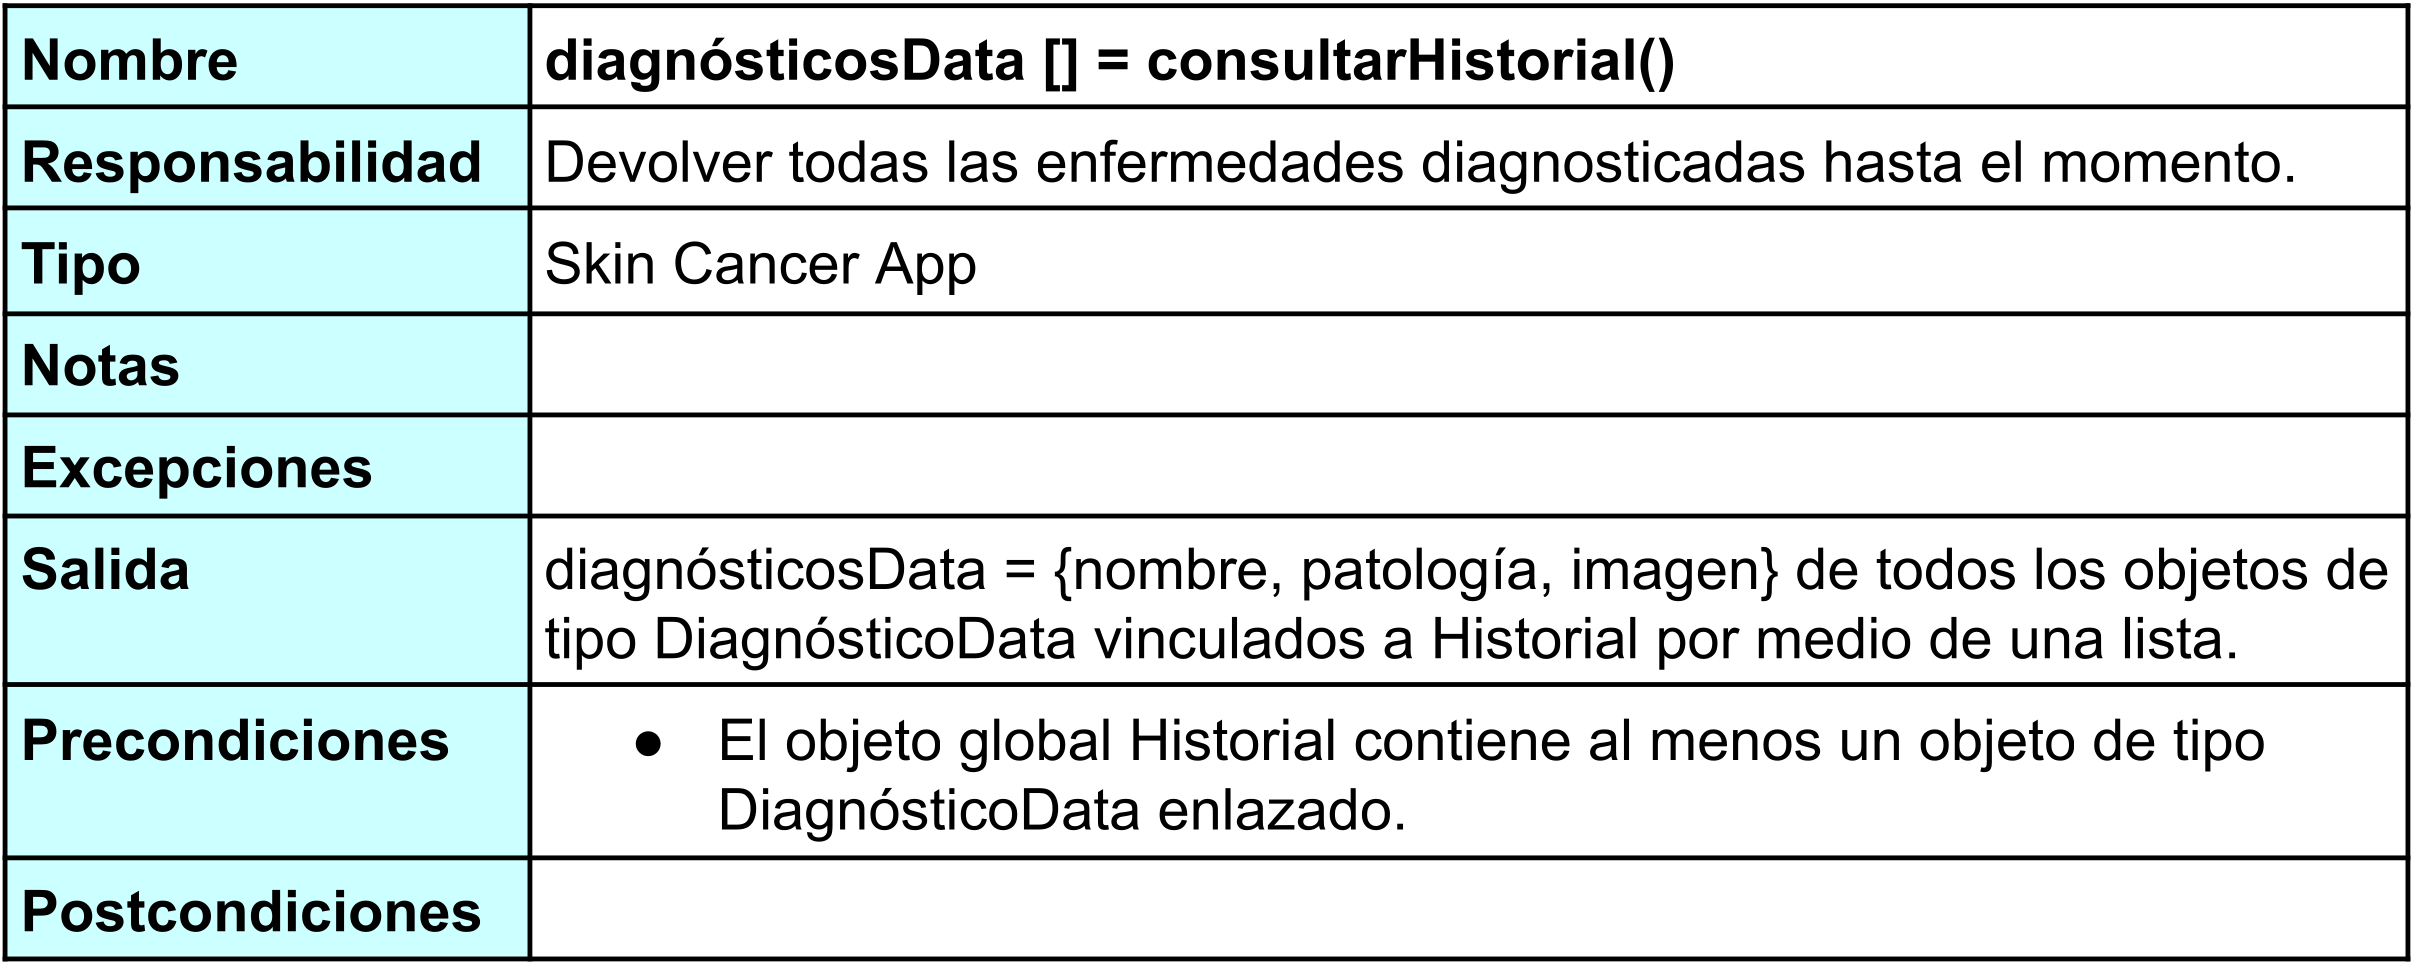
\includegraphics[scale = 0.16]{imagenes/contrato5.png}
 	\caption{Contrato: consultar historial.}
 	\label{fig:contrato5}
 \end{table}
 
    \begin{table}[H]
 	\centering
 	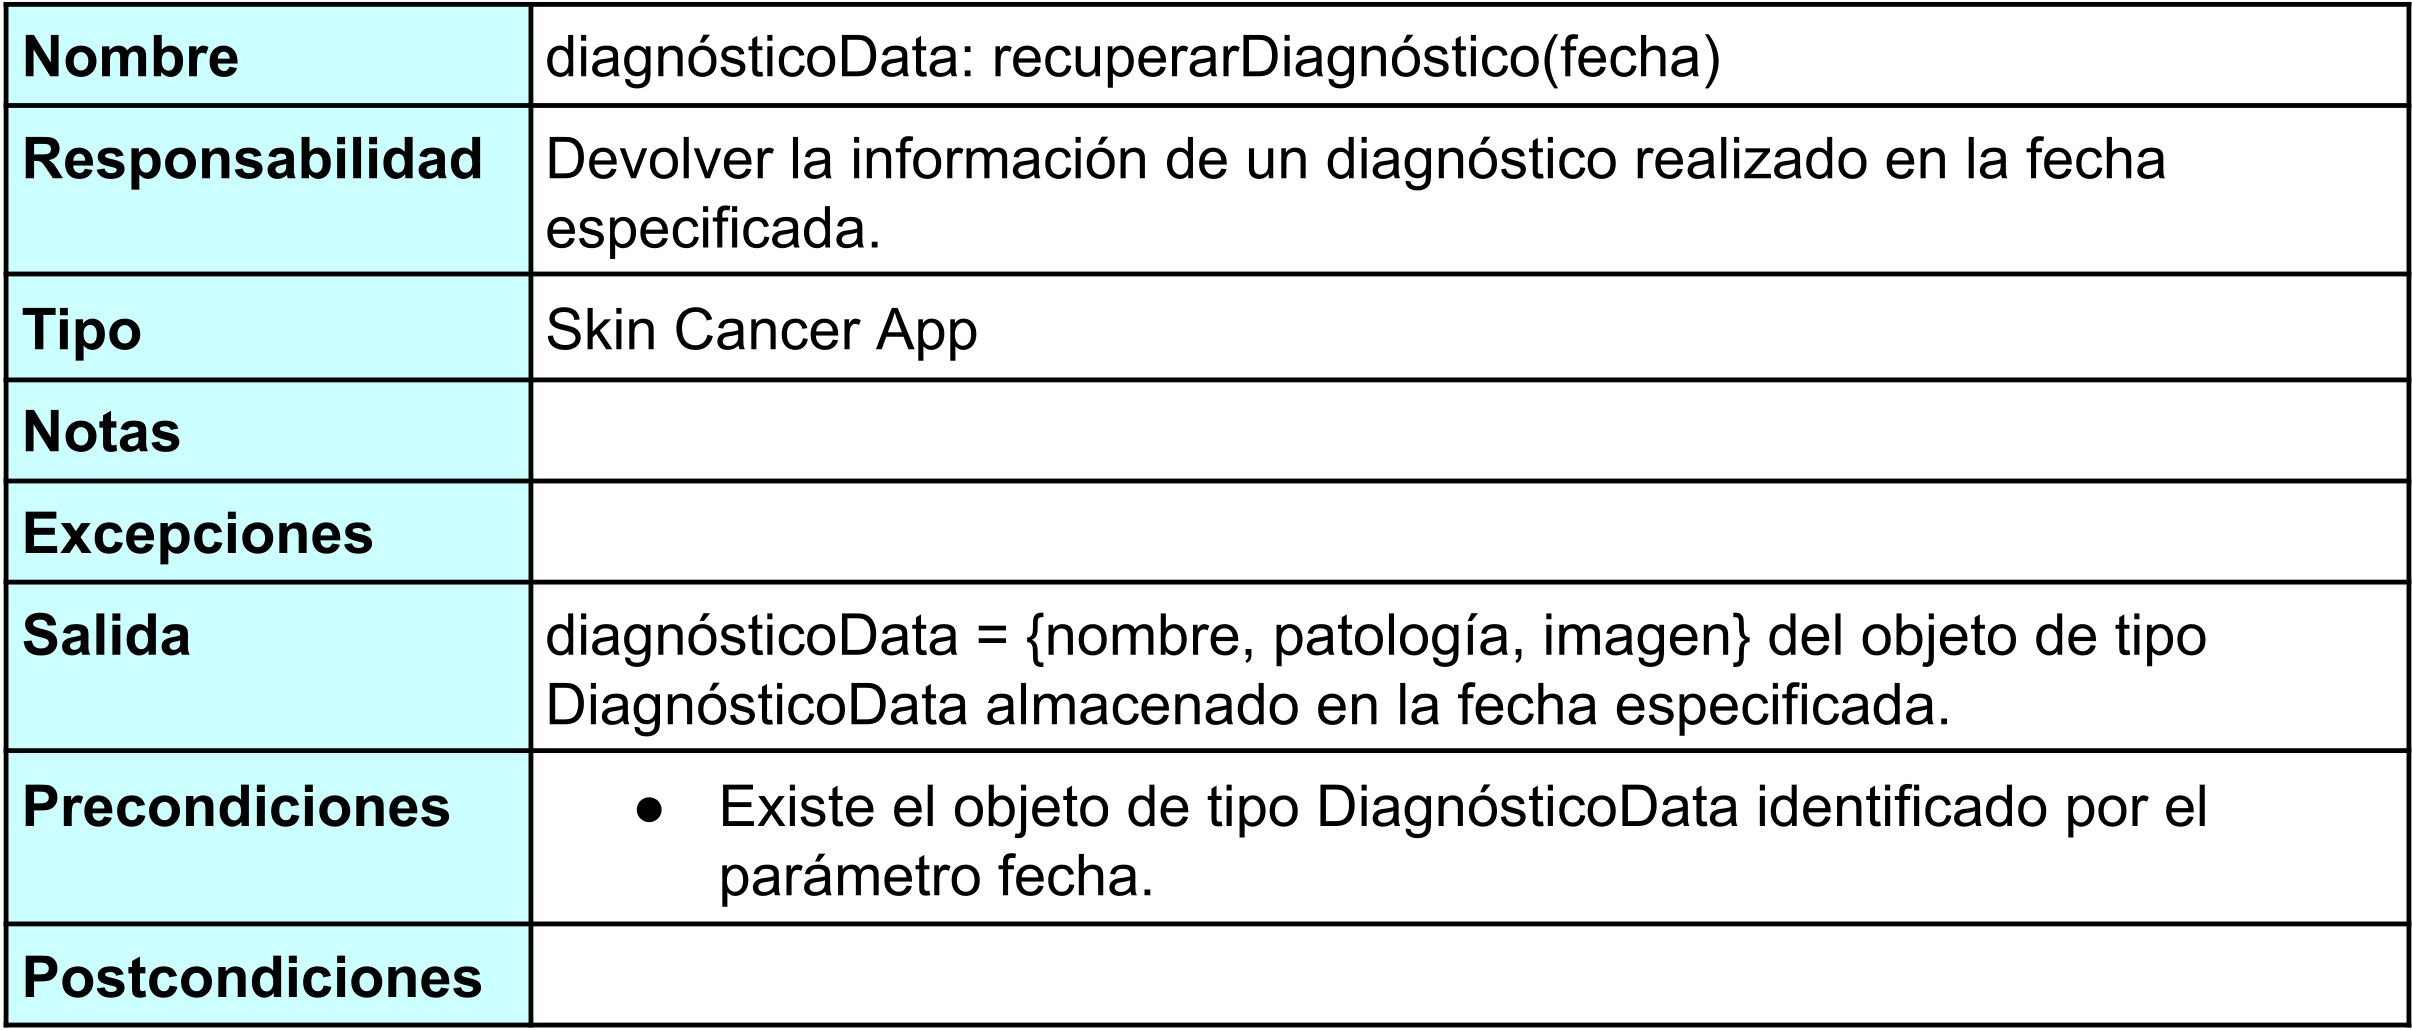
\includegraphics[scale = 0.16]{imagenes/contrato6.png}
 	\caption{Contrato: recuperar diagnóstico.}
 	\label{fig:contrato6}
 \end{table}
 
 Gracias a la definición formalizada en cada contrato, podemos trazar de forma específica los comportamientos de cada operación en diagramas de comunicación, para diseñar el modelo UML de clases de implementación, que describe la arquitectura definitiva del proyecto.
 
 \section{Diseño}
 
 La fase de diseño recoge la especificación final del sistema, teniendo como referencia los contratos y el diagrama conceptual asociado.
 
 En esta fase, llamada diseño por ser la fase previa a la implementación,  debemos crear los diagramas de comunicación (o interacción) de todas las
 operaciones especificadas en los contratos, y agregar posibles nuevas clases y atributos que no fueron especificados anteriormente, y que son requeridos para el correcto funcionamiento del sistema
 
 Toda esta información es recogida en el diagrama UML de clases del diseño, donde, partiendo del diagrama conceptual, se incluirán las clases con sus atributos y métodos, de los cuales se detallan la navegabilidad y la visibilidad de los atributos.
 
 \subsection{Diagramas de comunicación}
 
 Los diagramas de comunicación permiten observar con detalle el comportamiento interno de cada una de las operaciones del sistema. Si bien estas ya fueron especificadas en los contratos, el funcionamiento interno de la misma quedó en un segundo plano, ya que su objetivo era describir la operación sin entrar en detalles de implementación. Mediante los diagramas de comunicación presentes a continuación, podemos acercarnos un paso más a la implementación. Siguiendo el orden de los contratos, podemos encontrar los diagramas  en ese mismo orden: tomar fotografía (\ref{fig:com1}),  seleccionar imagen (\ref{fig:com2}), recortar región de una imagen (\ref{fig:com3}), realizar diagnóstico (\ref{fig:com4}), consultar historial (\ref{fig:com5}) y recuperar diagnóstico (\ref{fig:com6}).
 
\begin{figure}[H]
 	\centering
 	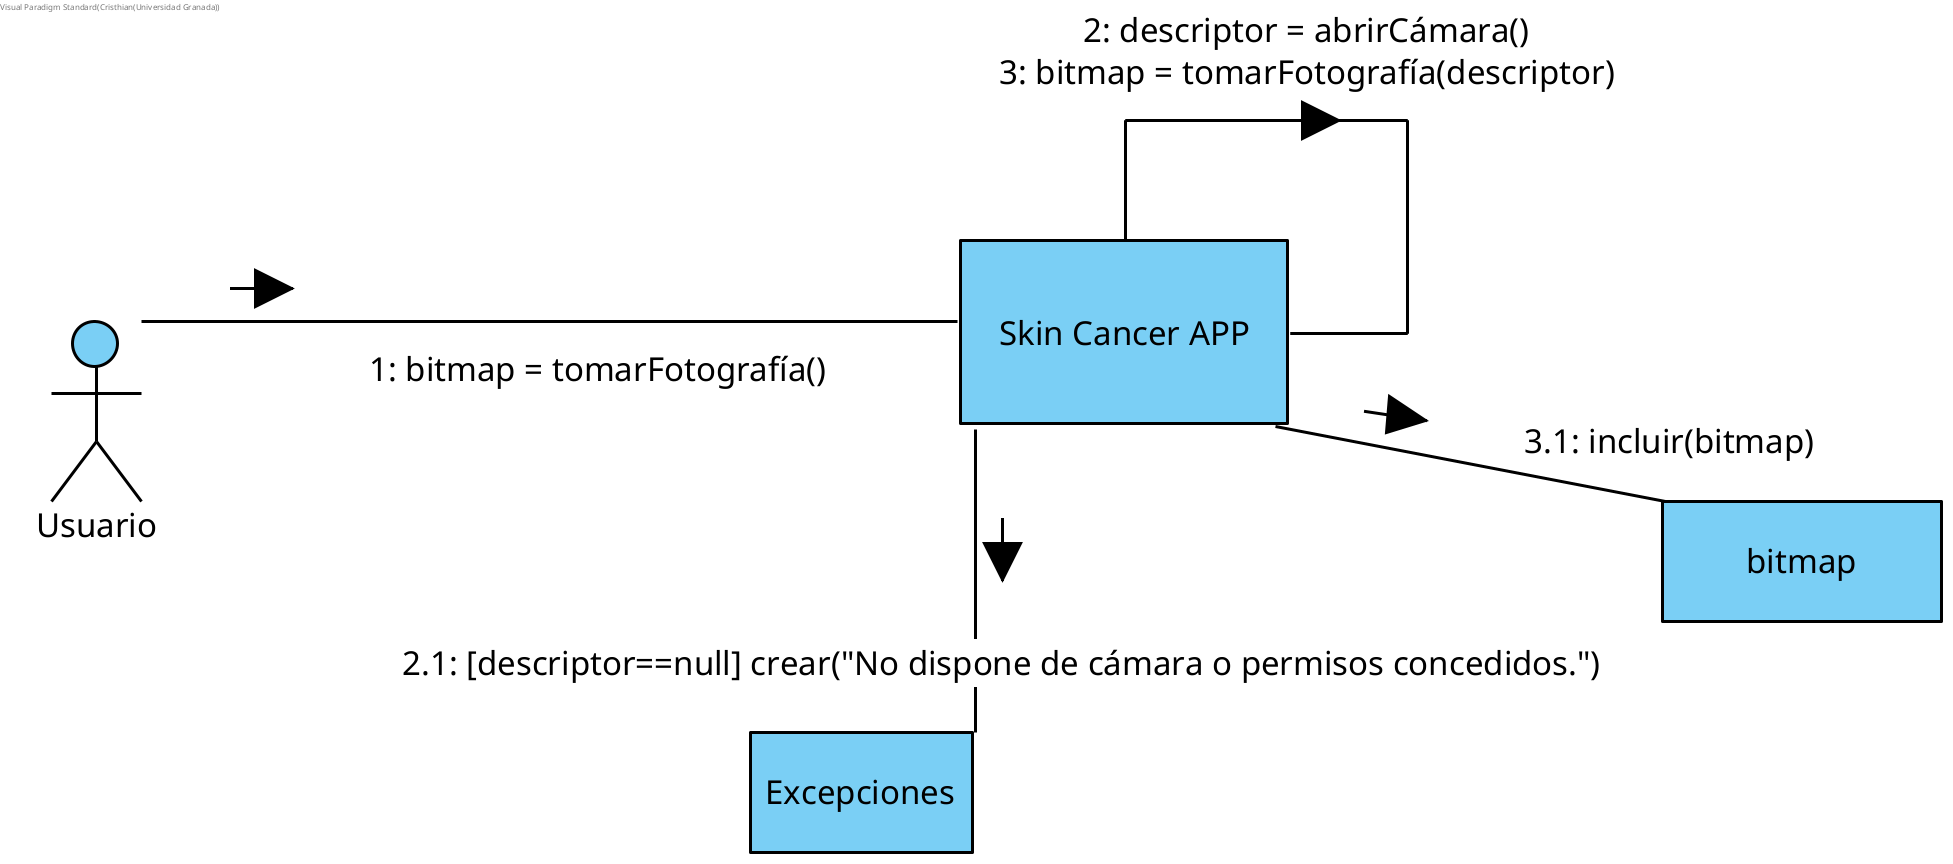
\includegraphics[scale = 0.8]{imagenes/TomarFotografía.png}
 	\caption{Diagrama de comunicación: recuperar diagnóstico.}
 	\label{fig:com1}
 \end{figure}
 
 
\begin{figure}[H]
 	\centering
 	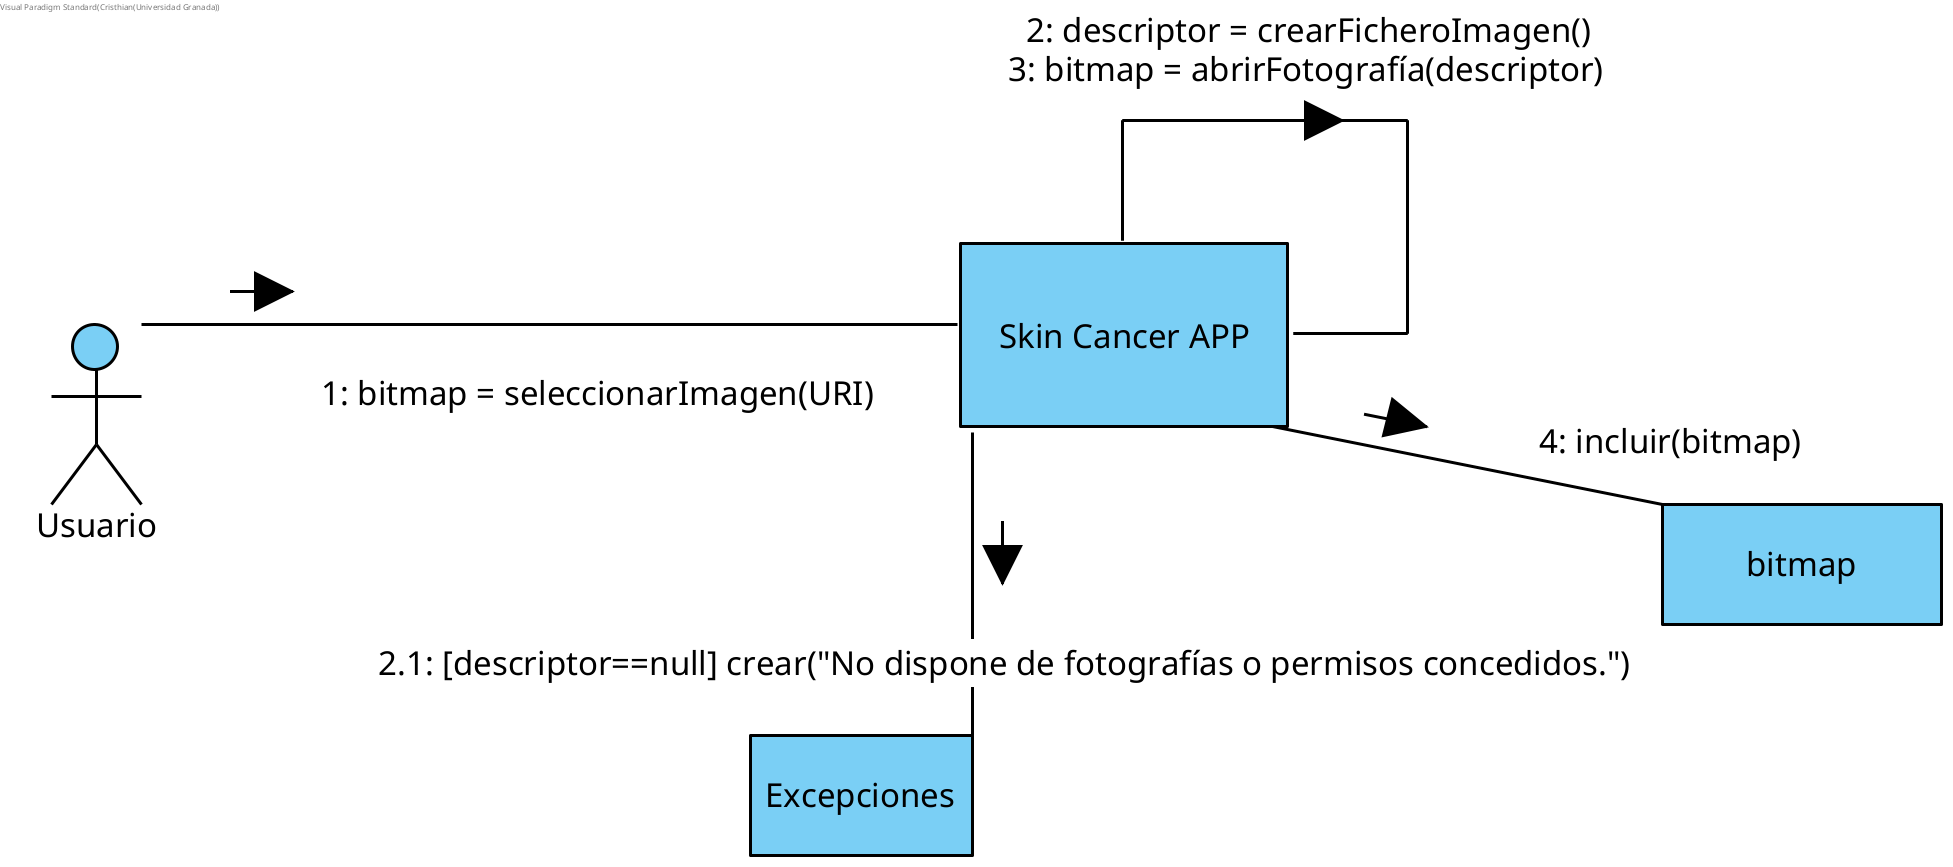
\includegraphics[scale = 0.8]{imagenes/SeleccionarImagen.png}
 	\caption{Diagrama de comunicación: seleccionar imagen}
 	\label{fig:com2}
 \end{figure}
 
\begin{figure}[H]
 	\centering
 	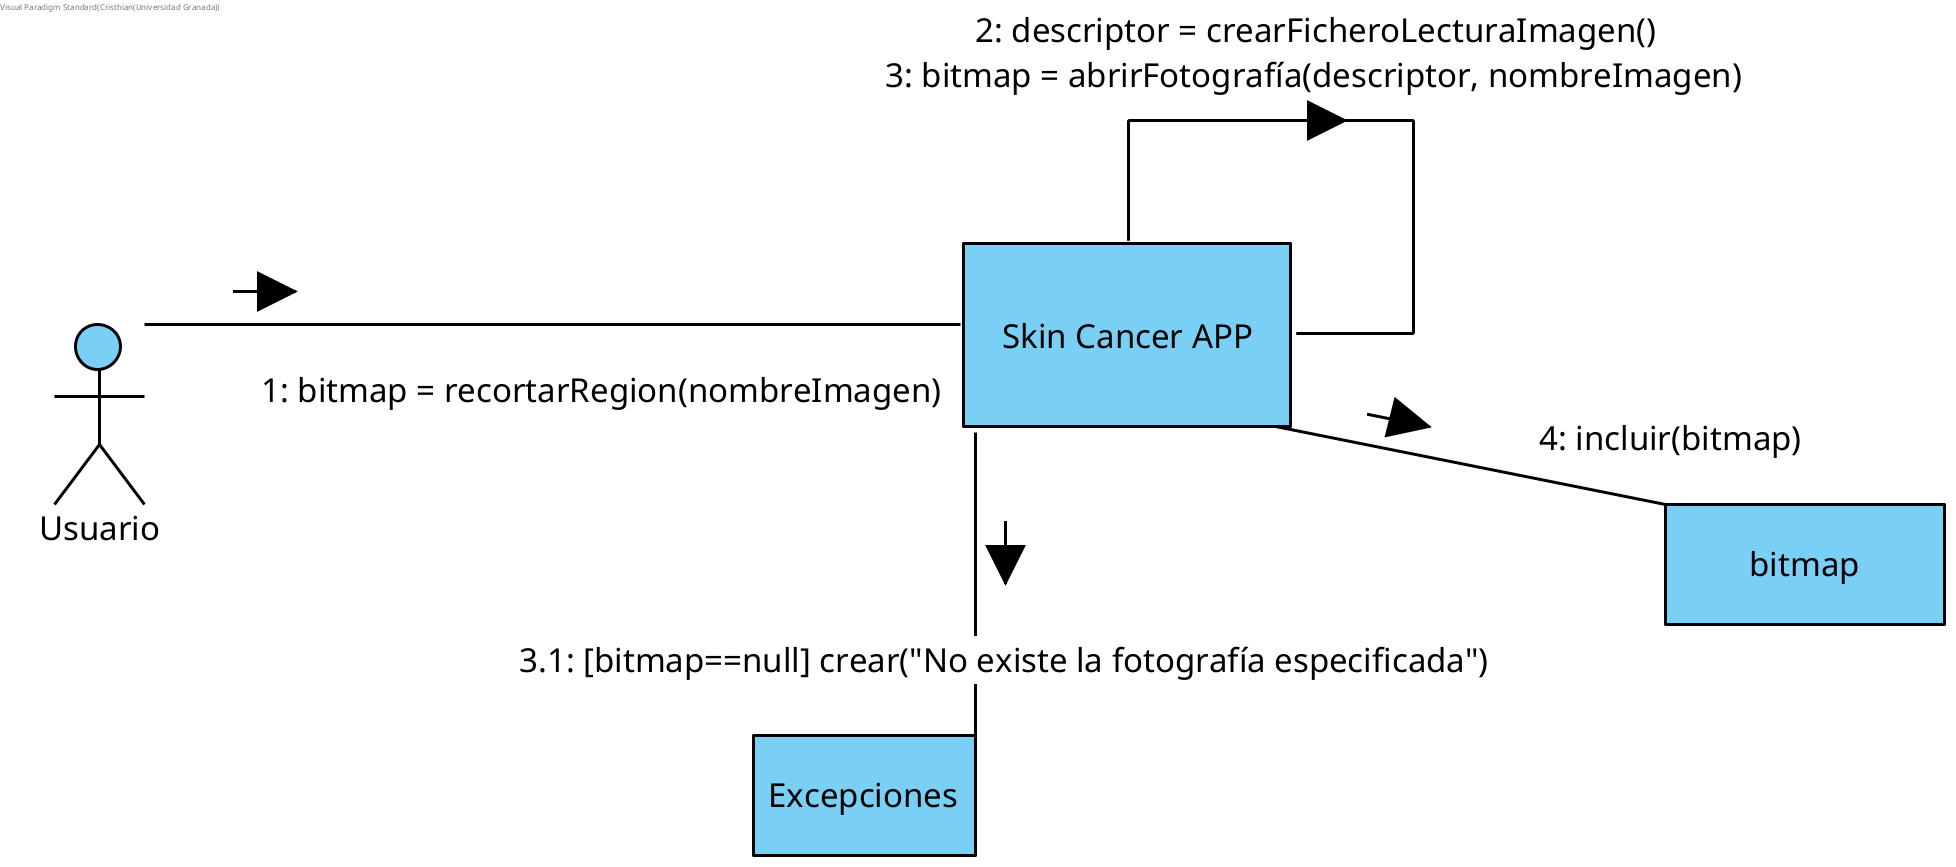
\includegraphics[scale = 0.8]{imagenes/RecortarRegión.png}
 	\caption{Diagrama de comunicación: recortar región}
 	\label{fig:com3}
 \end{figure}
 
 \begin{figure}[H]
 	\centering
 	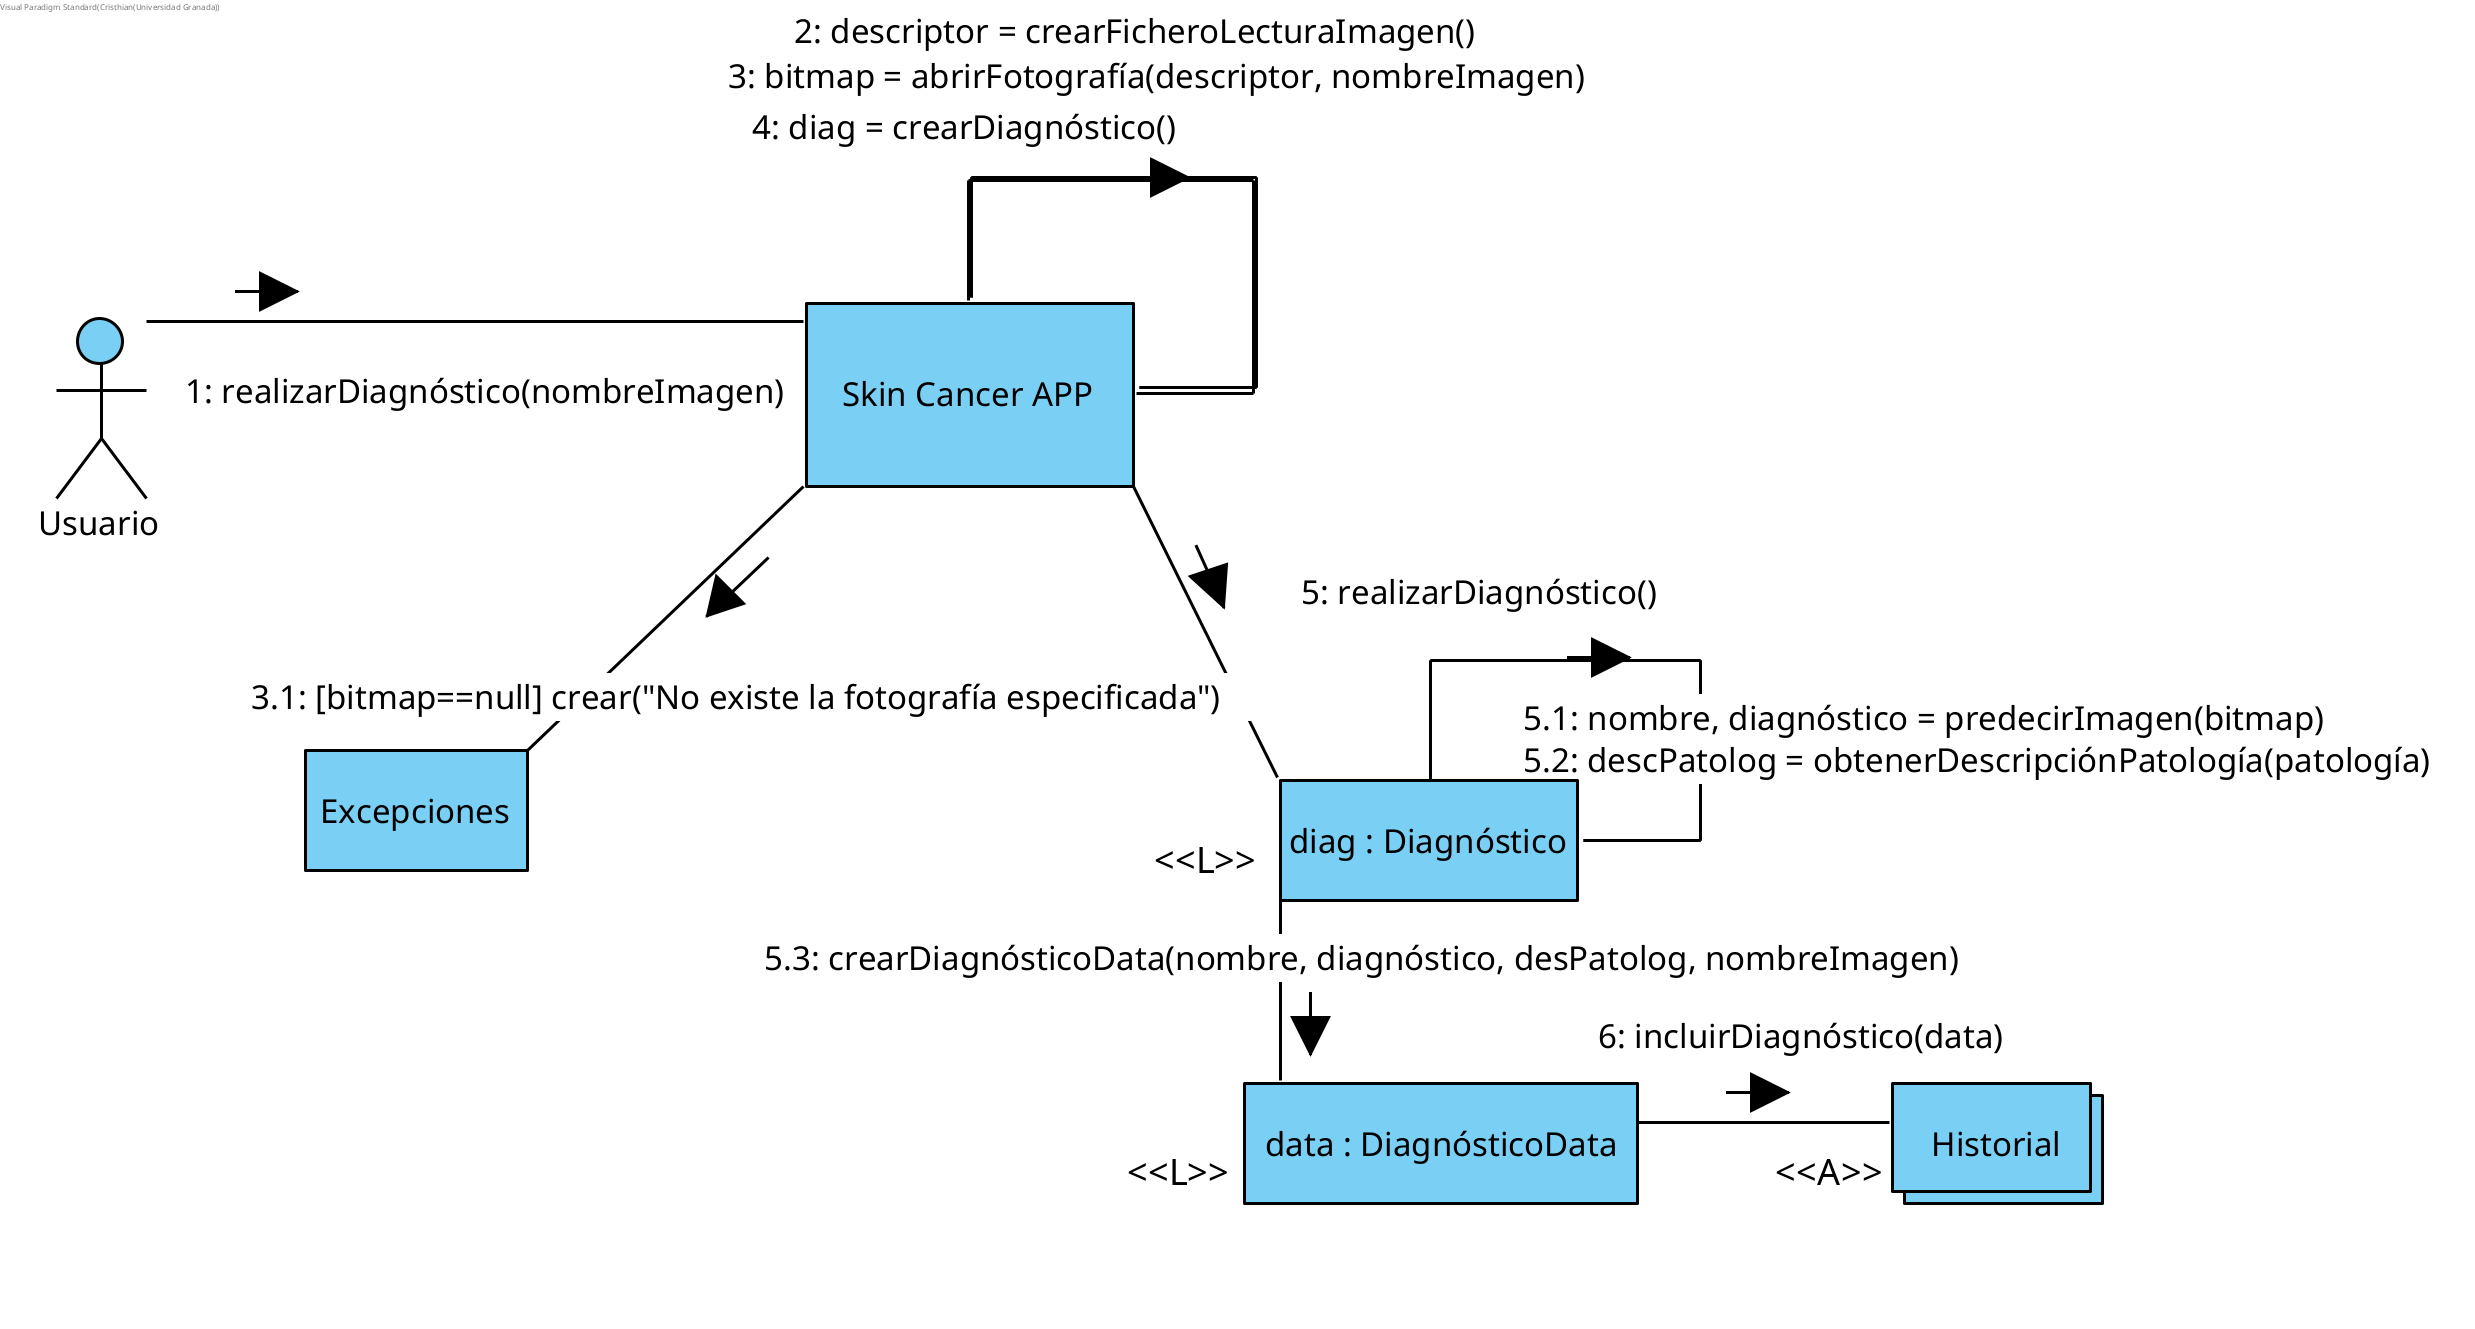
\includegraphics[scale = 0.75]{imagenes/RealizarDiagnóstico.png}
 	\caption{Diagrama de comunicación: realizar diagnóstico}
 	\label{fig:com4}
 \end{figure}
 
  \begin{figure}[H]
 	\centering
 	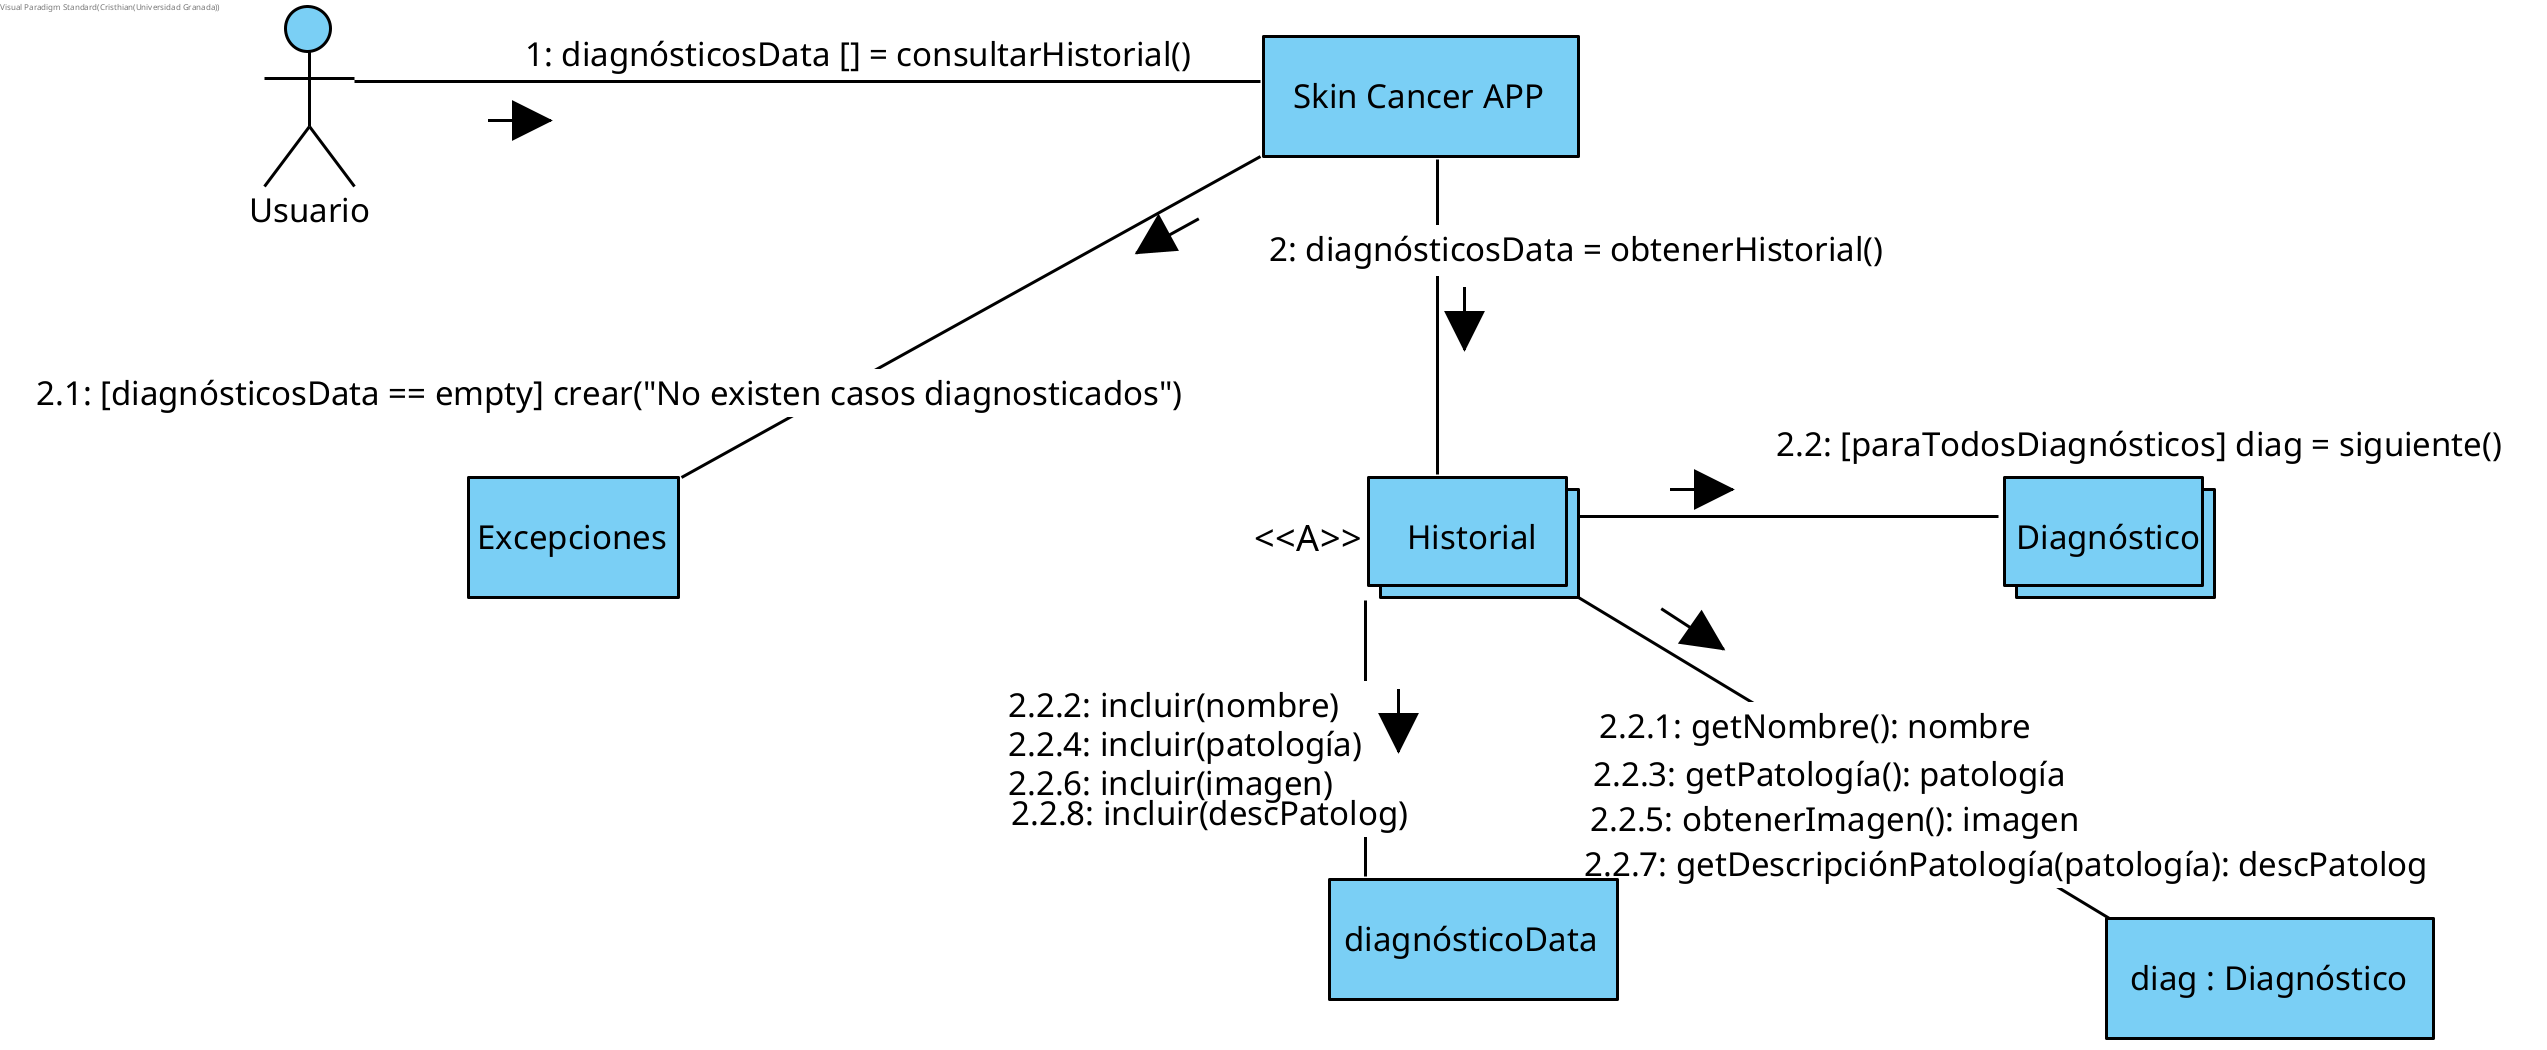
\includegraphics[scale = 0.75]{imagenes/HistorialSec.png}
 	\caption{Diagrama de comunicación: consultar historial}
 	\label{fig:com5}
 \end{figure}
 
 
   \begin{figure}[H]
 	\centering
 	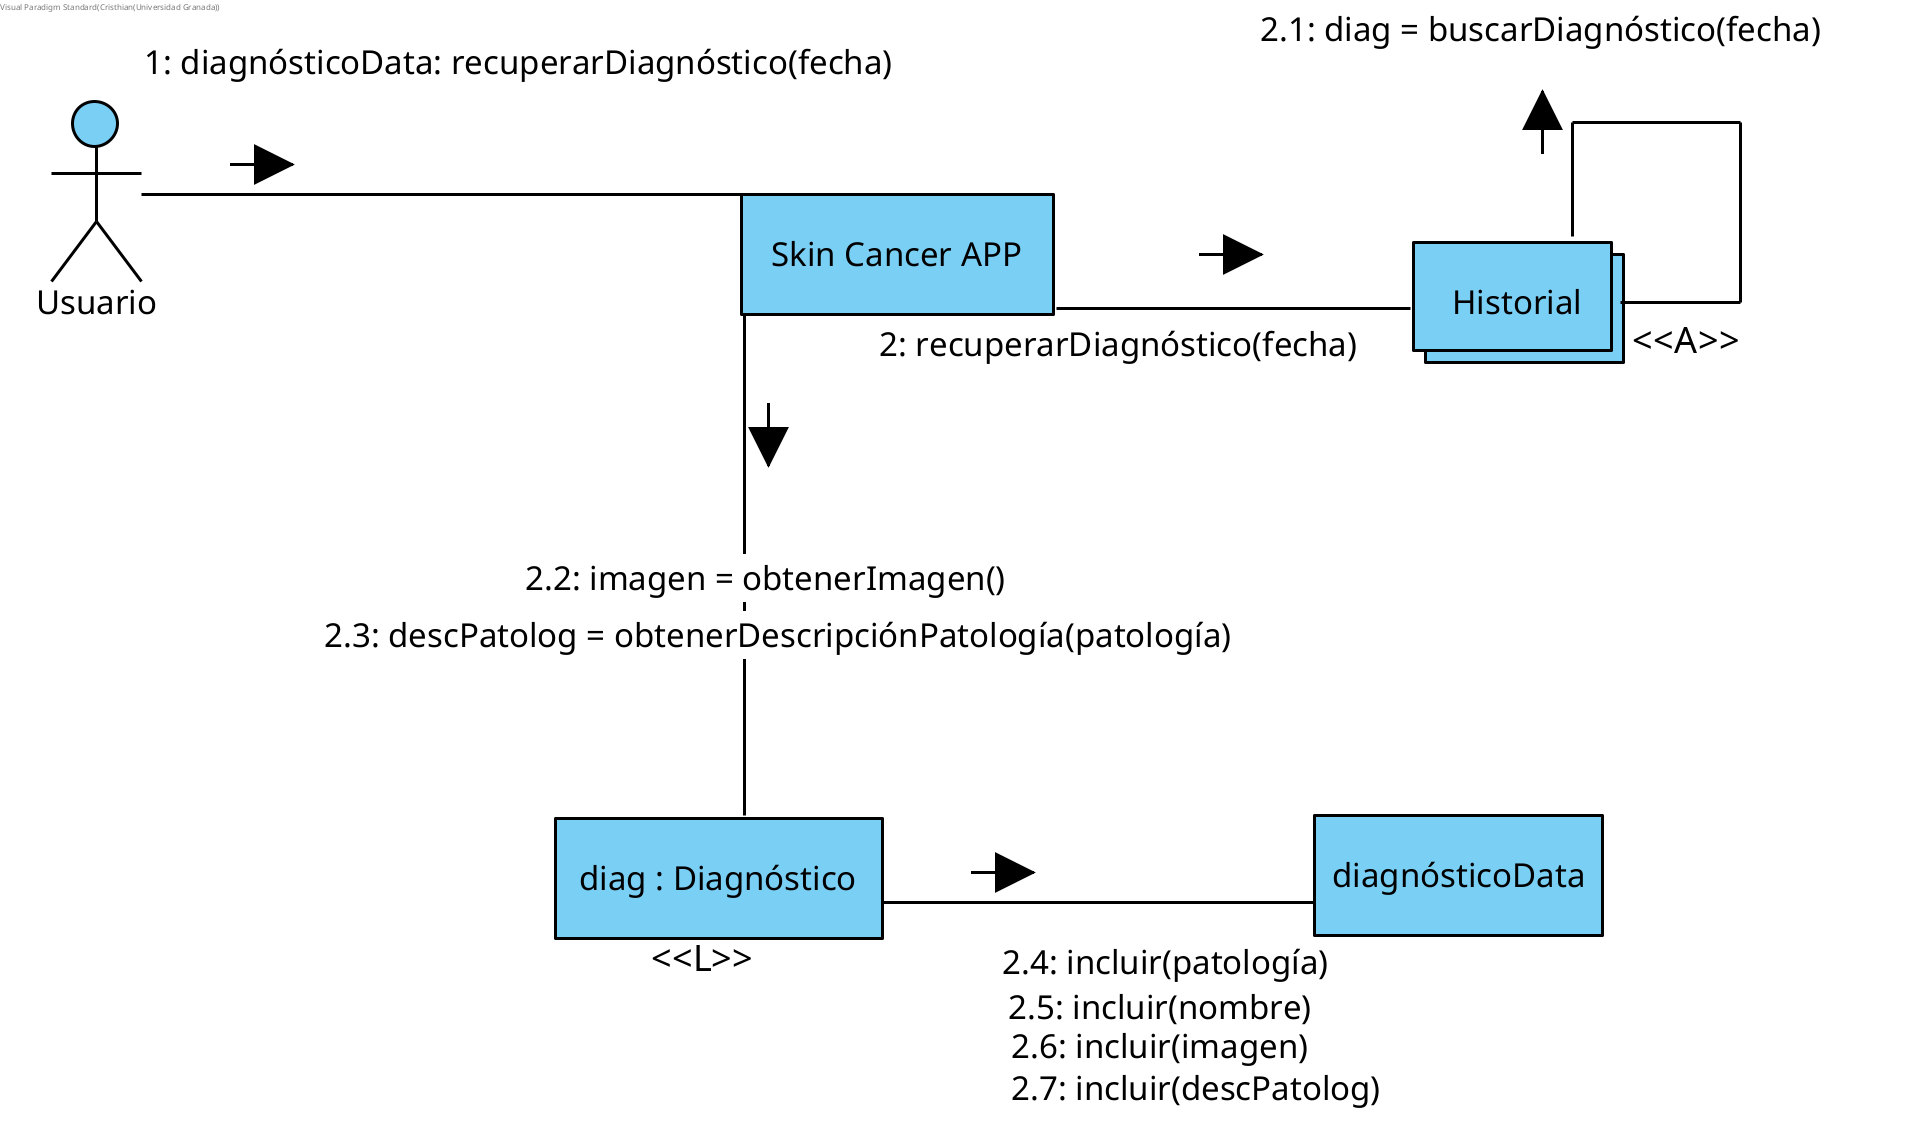
\includegraphics[scale = 0.75]{imagenes/GetDiagnóstico.png}
 	\caption{Diagrama de comunicación: consultar entrada de historial}
 	\label{fig:com6}
 \end{figure}
 
 Una vez establecido el comportamiento de forma específica, podemos pasar a la fase de creación del diagrama UML de clases.
 
 \subsection{Diagrama de clases de implementación}
 Este paso es el último antes de la implementación, por lo que debemos especificar adecuadamente cada una de las clases y métodos que realmente se requieren para crear la aplicación. La implementación se llevará a cabo empleando el IDE de Android Studio~\cite{androidstudio}, y siguiendo el patrón de implementación propuesto por Android.
  
 Su estructura es bastante diferente a la de un proyecto habitual; a pesar de emplear Java \cite{javalang} para la implementación de clases, la creación de una aplicación se centra en hacer uso de dos patrones principalmente: el uso de actividades y fragmentos, por lo que las clases presentes en el proyecto heredan de estas dos clases y producen cambios sustanciales en la estructura originalmente ideada. Si profundizamos en los conceptos de fragmento y actividad:
 
 \begin{itemize}
 	\item \textbf{Actividad}~\cite{actividad}: es la unidad básica de ejecución de una aplicación Android, y permite mostrar el contenido de la aplicación. El ciclo de vida de una actividad comprende la creación de la misma, hasta su destrucción, cuando el sistema recupera los recursos de esa actividad. Es posible navegar entre actividades, realizando su declaración adecuadamente, aunque, como última tendencia, se suelen emplear fragmentos para realizar cambios de ventana.
 	\item \textbf{Fragmento}~\cite{fragmento}: es una parte modular de la interfaz de usuario, la cual posee un ciclo vida con varias fases; principalmente, usaremos creación (método onCreate), destrucción (onDestroy) y actualización del contenido, mediante métodos implementados por nosotros mismos. Permite recoger las entradas y salidas del usuario, y normalmente, dependen de una actividad para funcionar.
 \end{itemize}
 
 Por tanto, al heredar de estas clases, deben incorporar los métodos de creación y destrucción, así como de actualización de información, y podemos obtener 3 subsistemas bien diferenciados: la pantalla de bienvenida de la aplicación, puramente informativa; el subsistema de diagnóstico y el subsistema de historial, siendo estos dos últimos los definidos en fases previas de esta tarea de diseño, pero que han requerido las modificaciones pertinentes para funcionar adecuadamente en el ecosistema Android.
 
 Podemos encontrar una visión general del sistema en el diagrama de la figura \ref{fig:clasesglobal}, así como una implementación del sistema de diagnóstico en la figura \ref{fig:clasesdiag} y el historial en la figura \ref{fig:claseshist}.
 
    \begin{figure}[H]
 	\centering
 	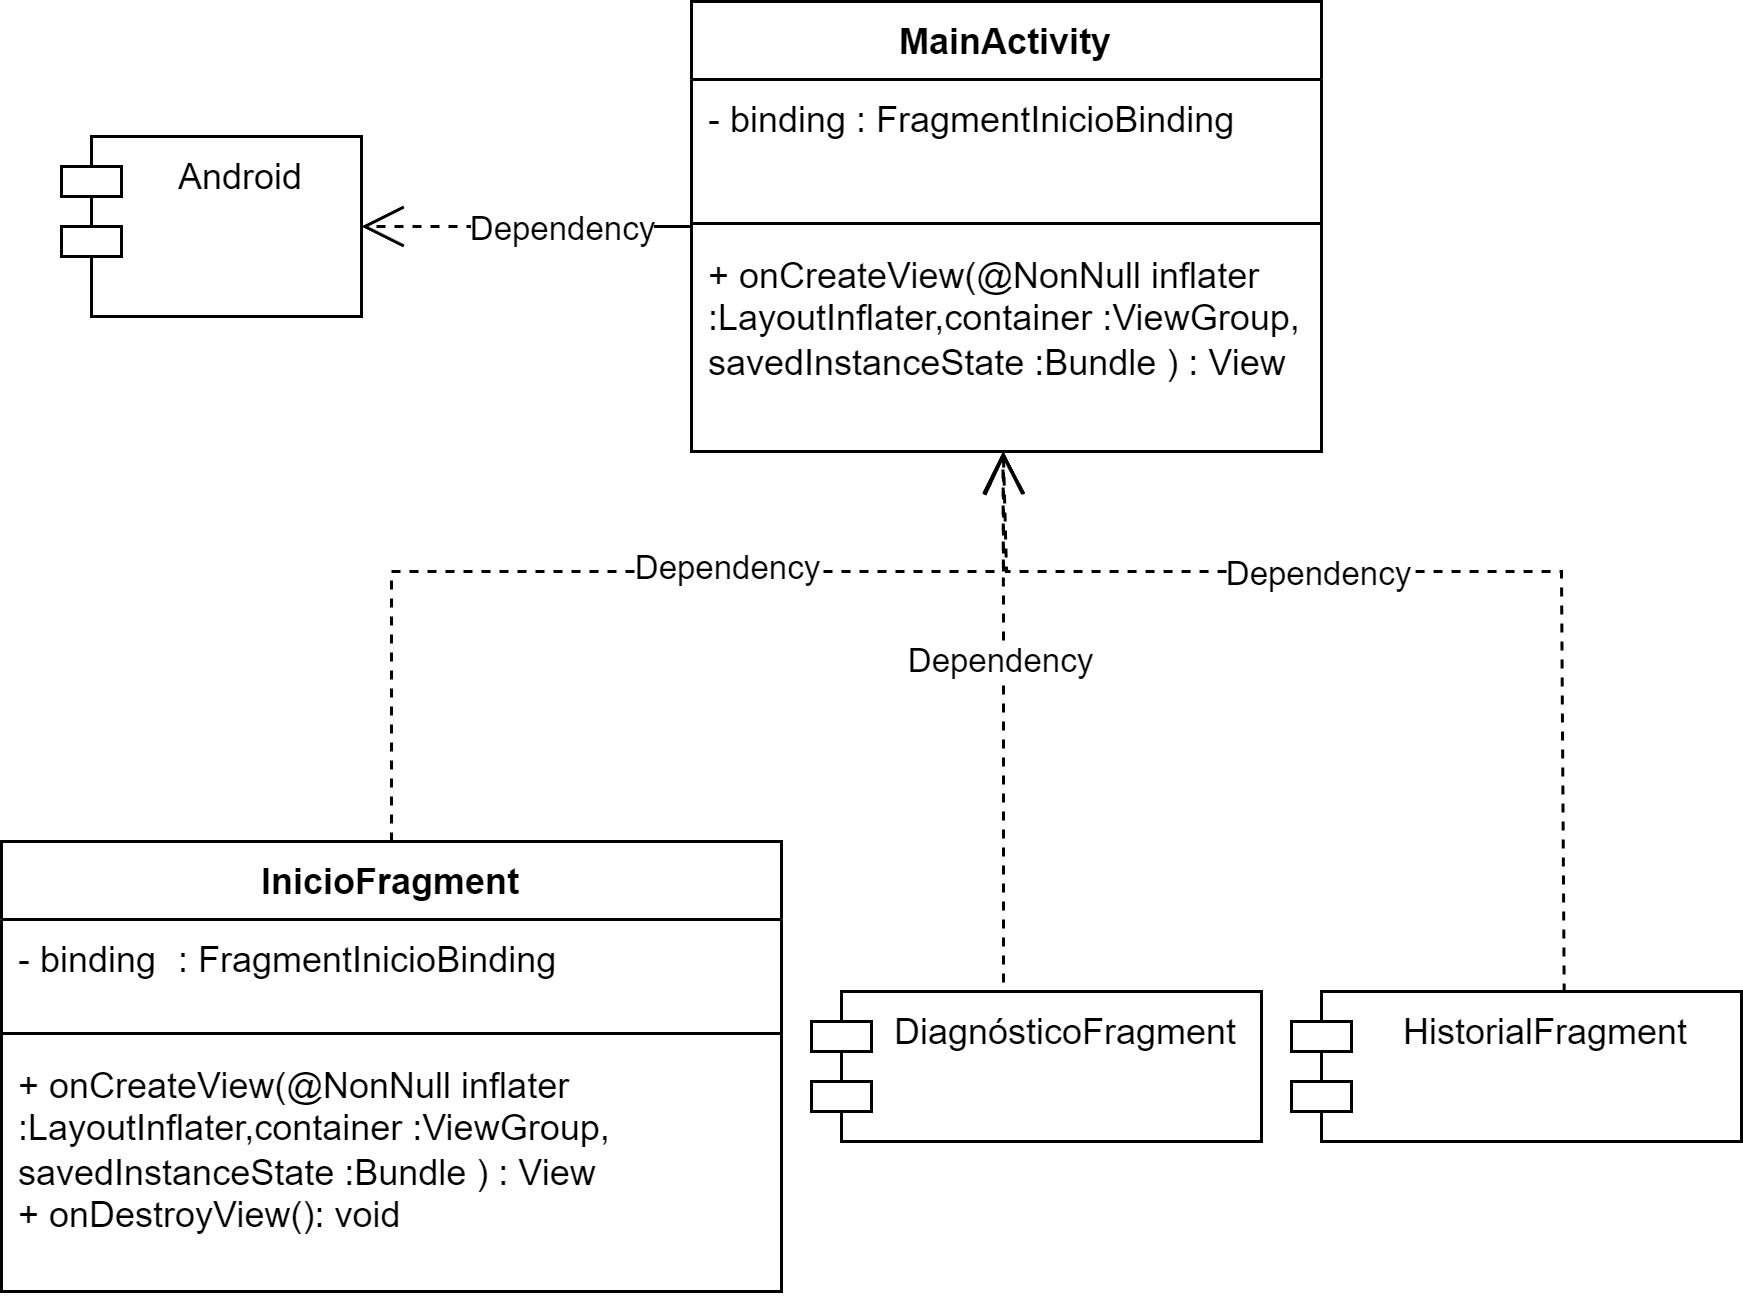
\includegraphics[scale = 0.75]{imagenes/DiagramaGeneral.png}
 	\caption{Diagrama de clases: visión general del sistema}
 	\label{fig:clasesglobal}
 \end{figure}
 
     \begin{figure}[H]
 	\centering
 	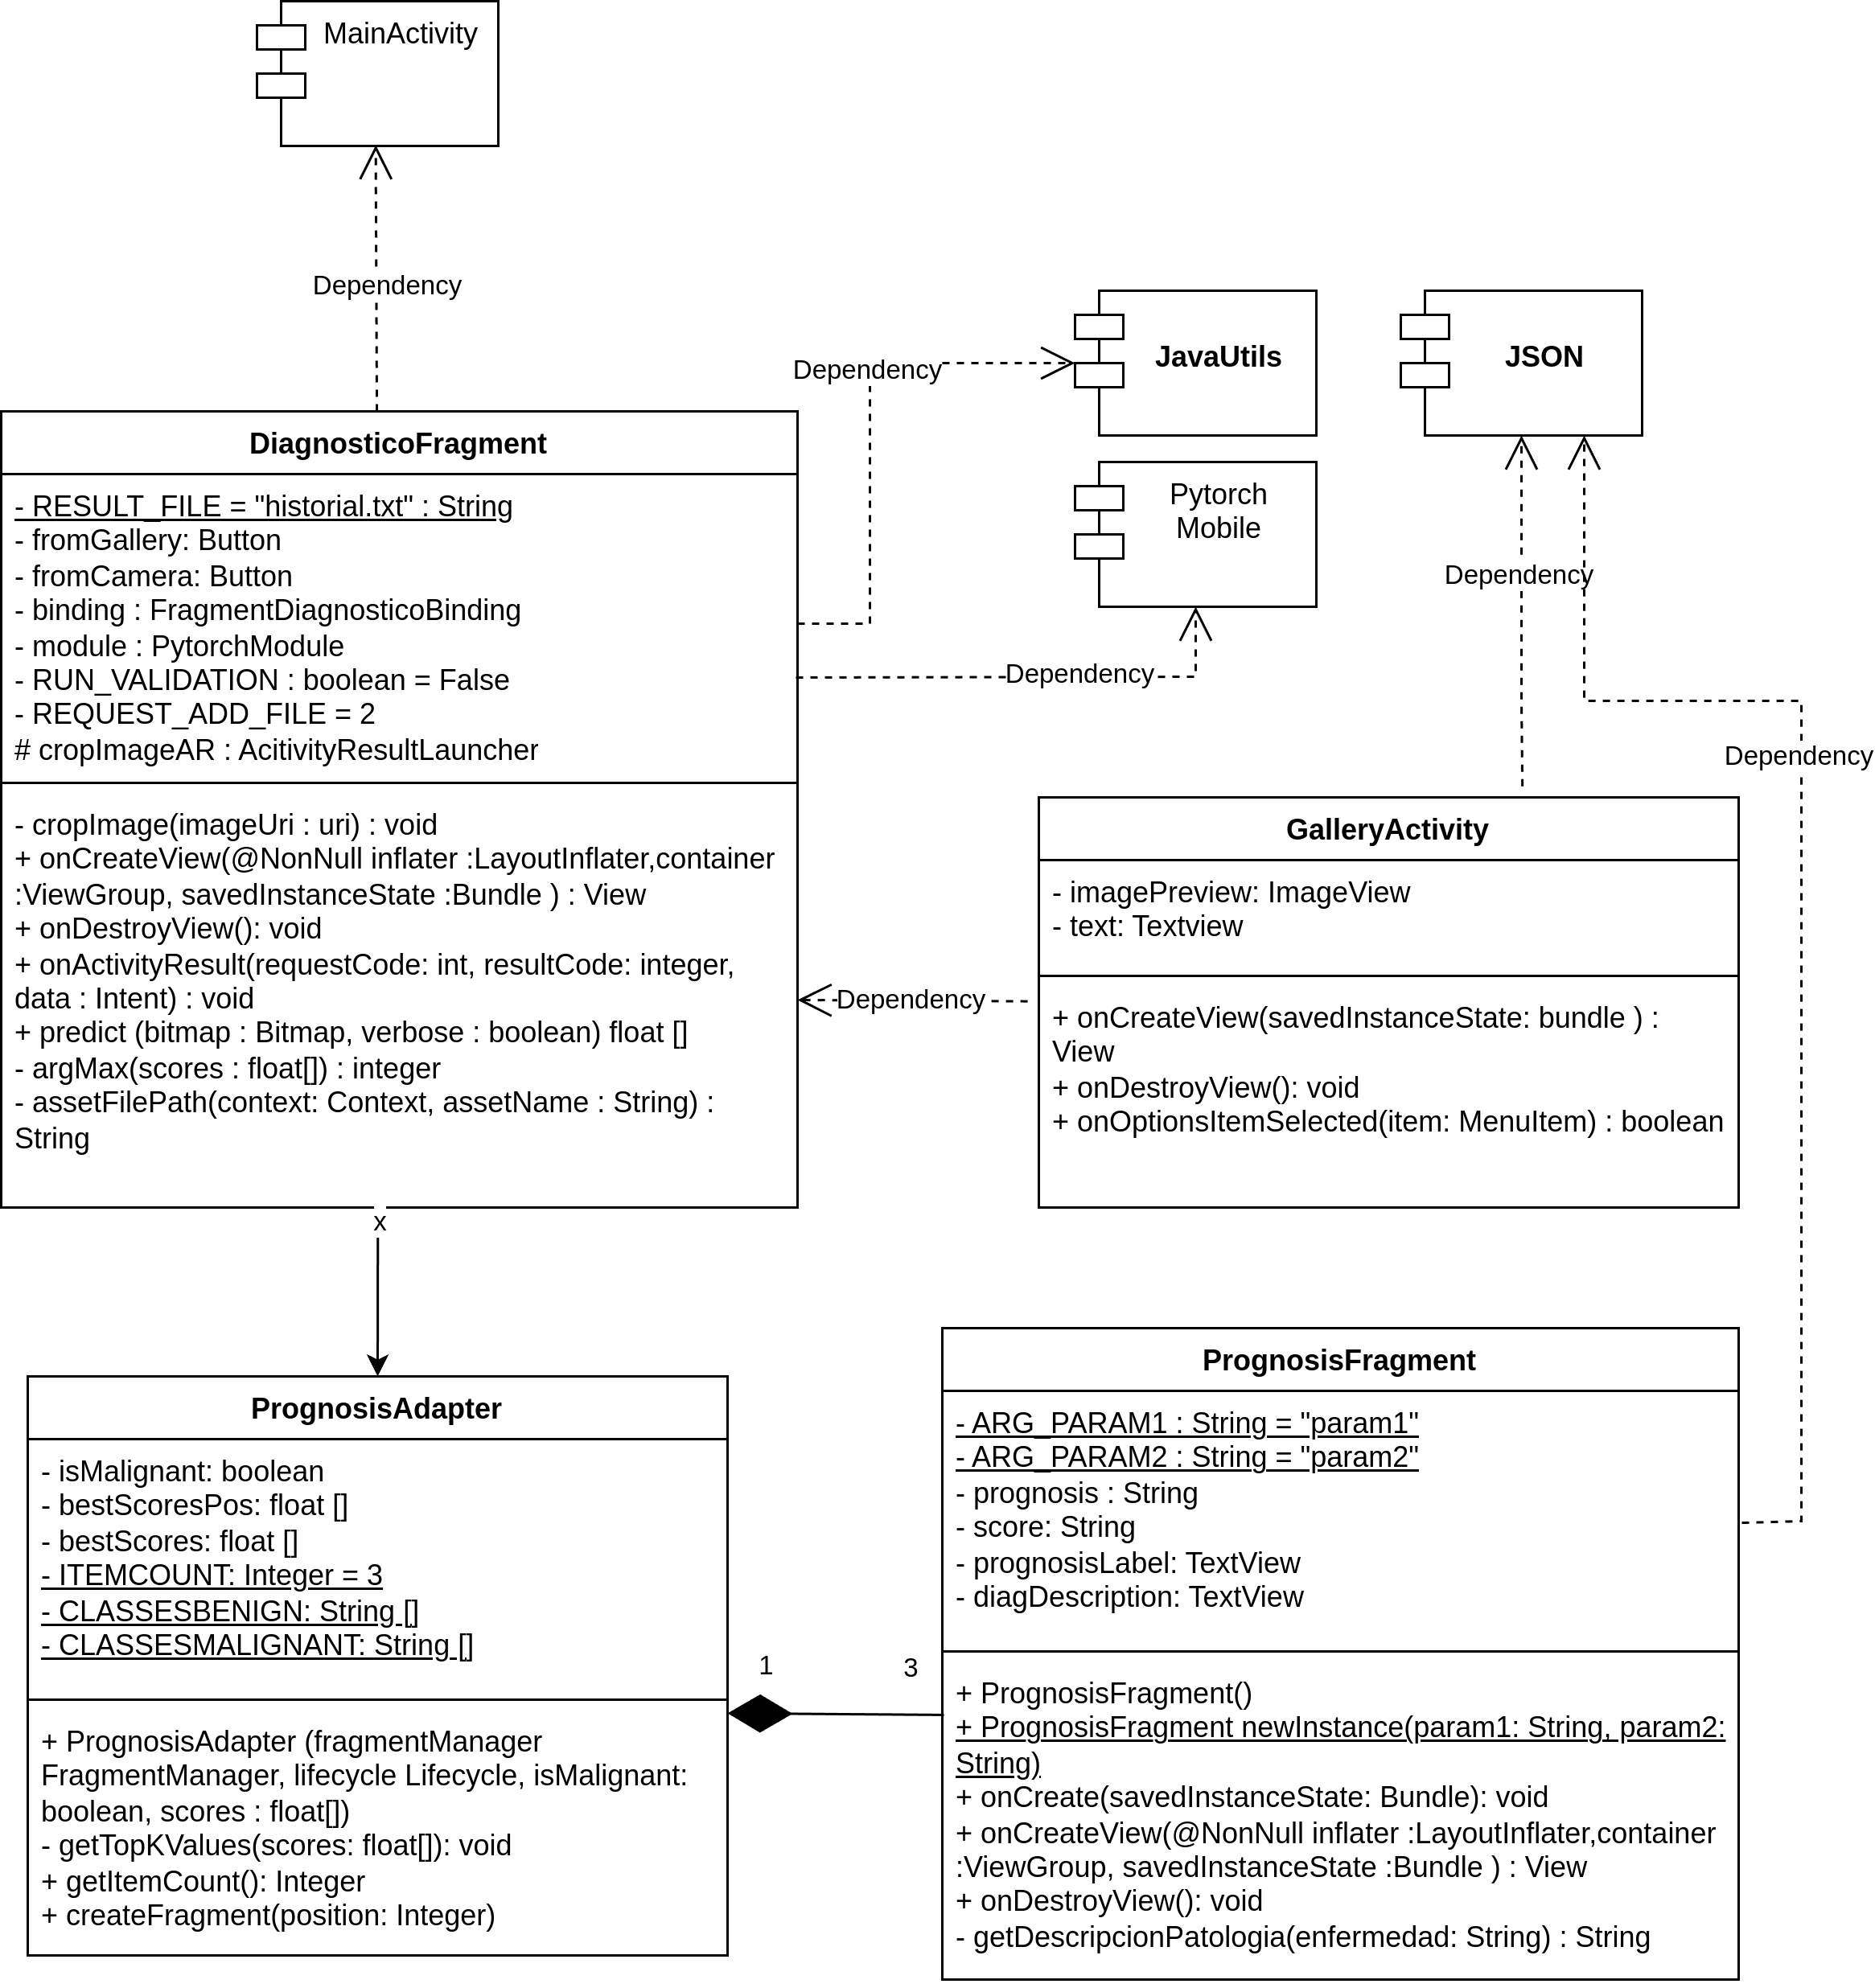
\includegraphics[scale = 0.75]{imagenes/androidAPP-Diagnostico.png}
 	\caption{Diagrama de clases: subsistema de diagnósticos}
 	\label{fig:clasesdiag}
 \end{figure}
 
      \begin{figure}[H]
 	\centering
 	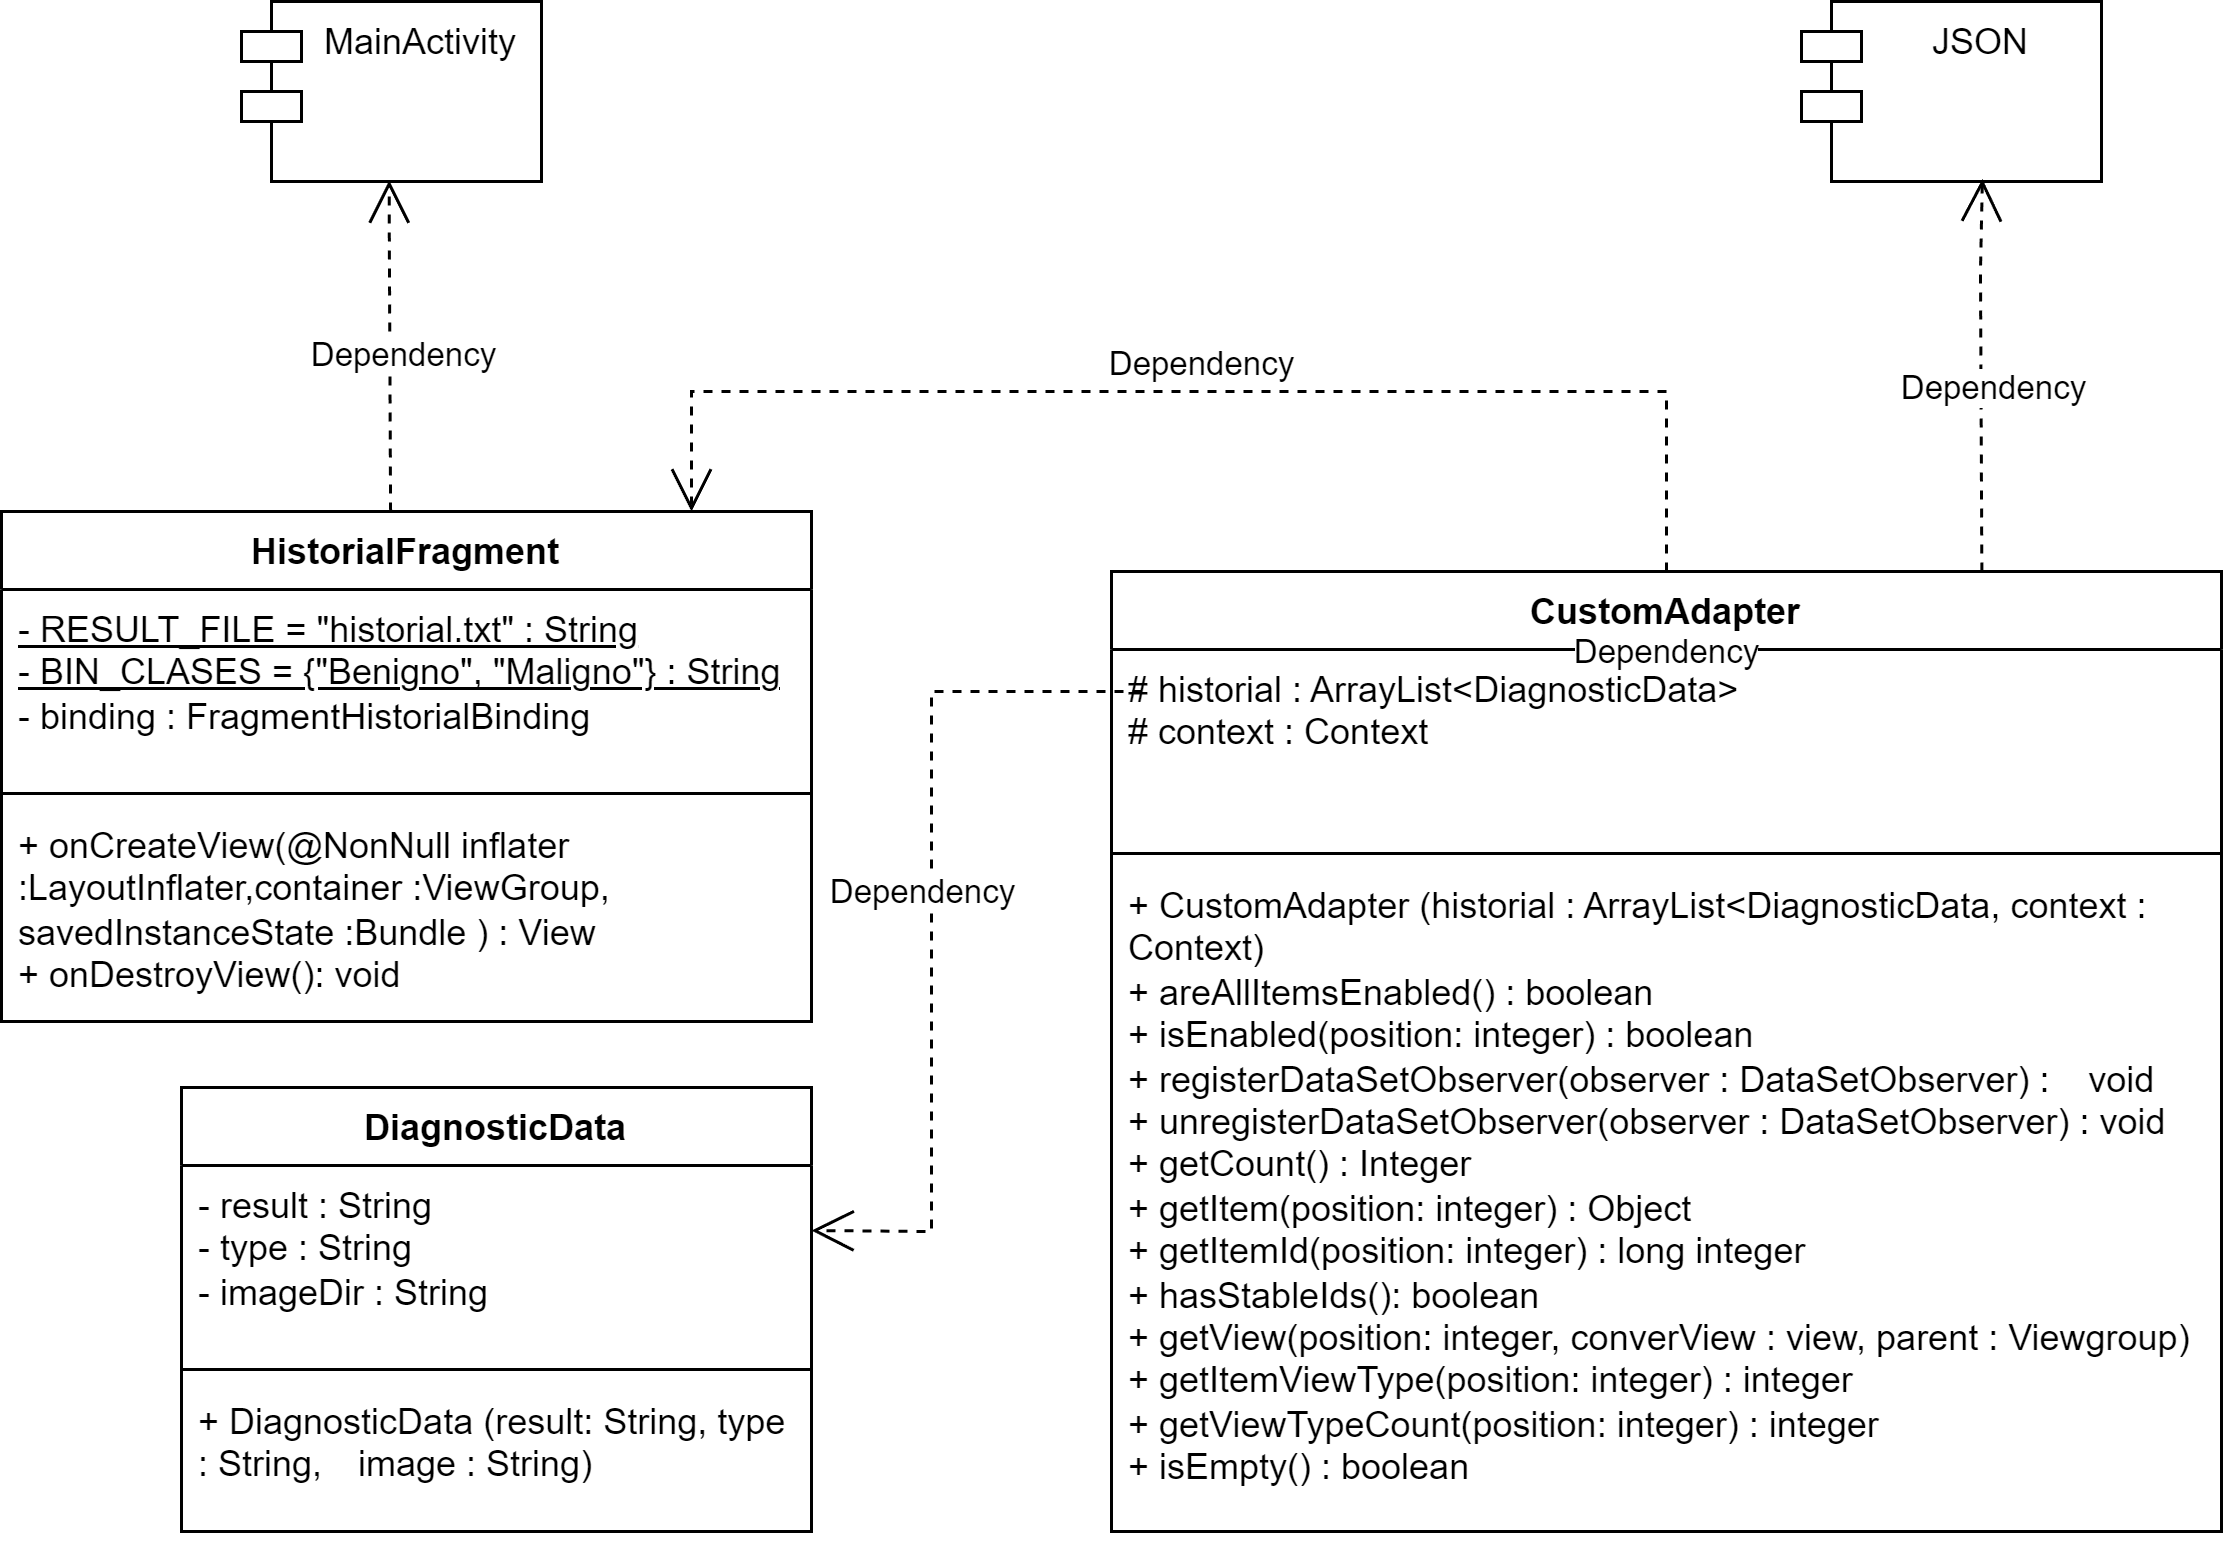
\includegraphics[scale = 0.75]{imagenes/androidAPP-Historial.png}
 	\caption{Diagrama de clases: subsistema de historial}
 	\label{fig:claseshist}
 \end{figure}
 
 \section{Manual de uso de la aplicación}
 En este apartado, se muestra el comportamiento de la aplicación y todas las funcionalidades disponibles para facilitar al usuario su funcionamiento.  Aunque la aplicación muestra mensajes de retroalimentación y descripciones en la interfaz, destacaremos en este apartado de forma visual toda su disposición.
 
 Nada más proceder con su apertura, podemos encontrar 3 submenús distintos si hacemos uso del panel lateral de navegación (apreciable en la figura  \ref{fig:inicioapp}):
 \begin{itemize}
 	\item  \textbf{Pantalla de bienvenida}. Página principal al iniciar la aplicación. Muestra información previa acerca de la utilidad de la aplicación, consejos de cuidados para la piel, y una exención de responsabilidades, donde se informa del propósito plenamente informativo del producto (ver figura \ref{fig:inicioapp}).
 	\item \textbf{Sección de diagnóstico}. Menú que coincide con la descrita en los diagramas anteriores, en la cual el usuario puede especificar una imagen de galería o mediante la cámara para ser diagnosticada. Se explica con detalle en la sección \ref{sec:diag}.
 	\item \textbf{Sección de historial}. Menú en forma lista que muestra todos los casos diagnosticados por el paciente. Permite ver la imagen analizada, y la información del diagnóstico realizado. Profundizado en la sección \ref{sec:hist}.
 \end{itemize}
 
   \begin{figure}[H]
 	\centering
 	\subfigure[Pantalla de inicio]{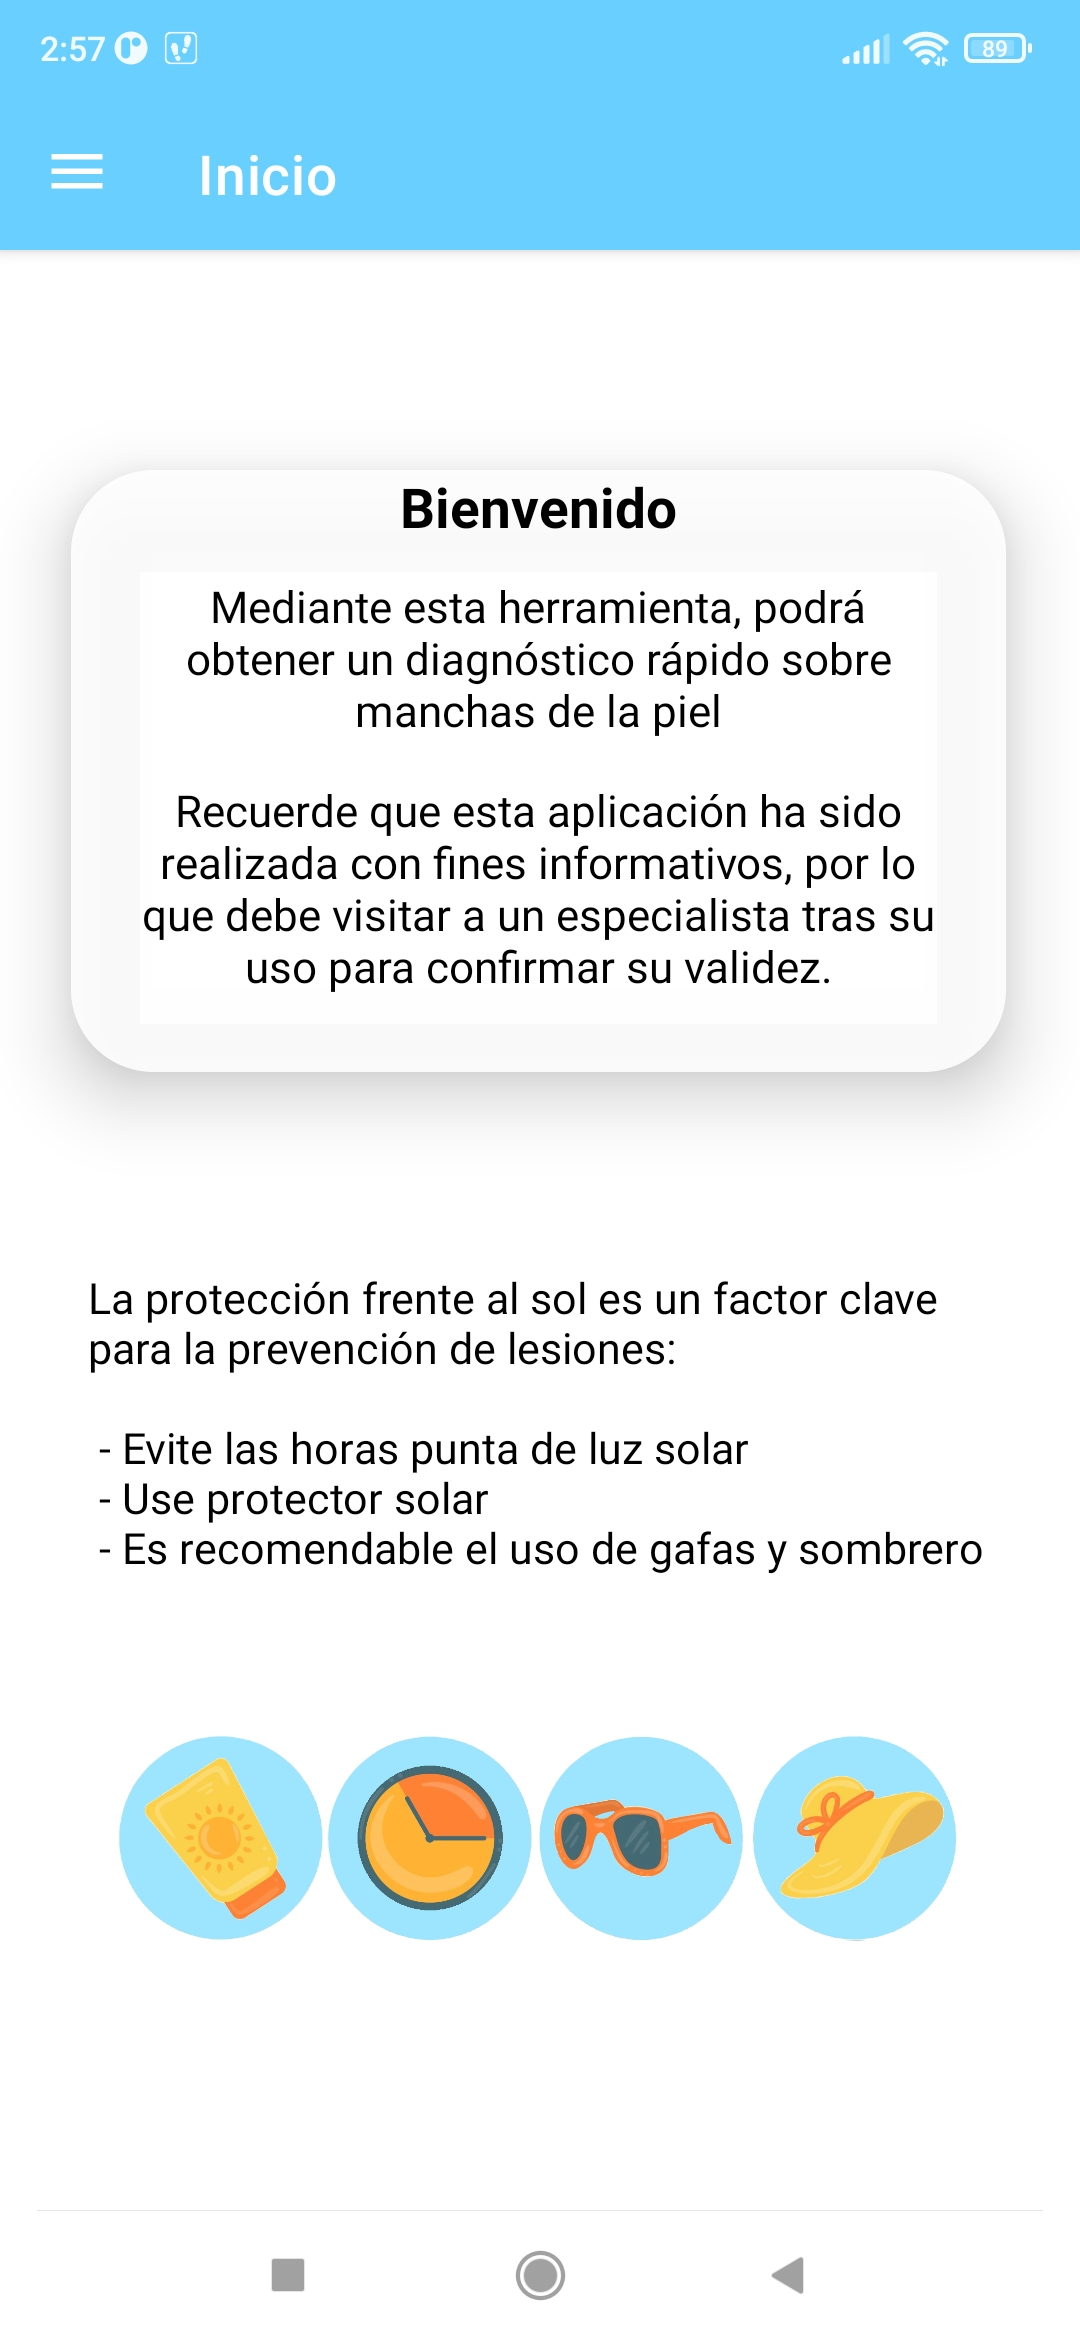
\includegraphics[scale = 0.125]{imagenes/bievenidaapp.jpg}}
 	 \subfigure[Menú de navegación]{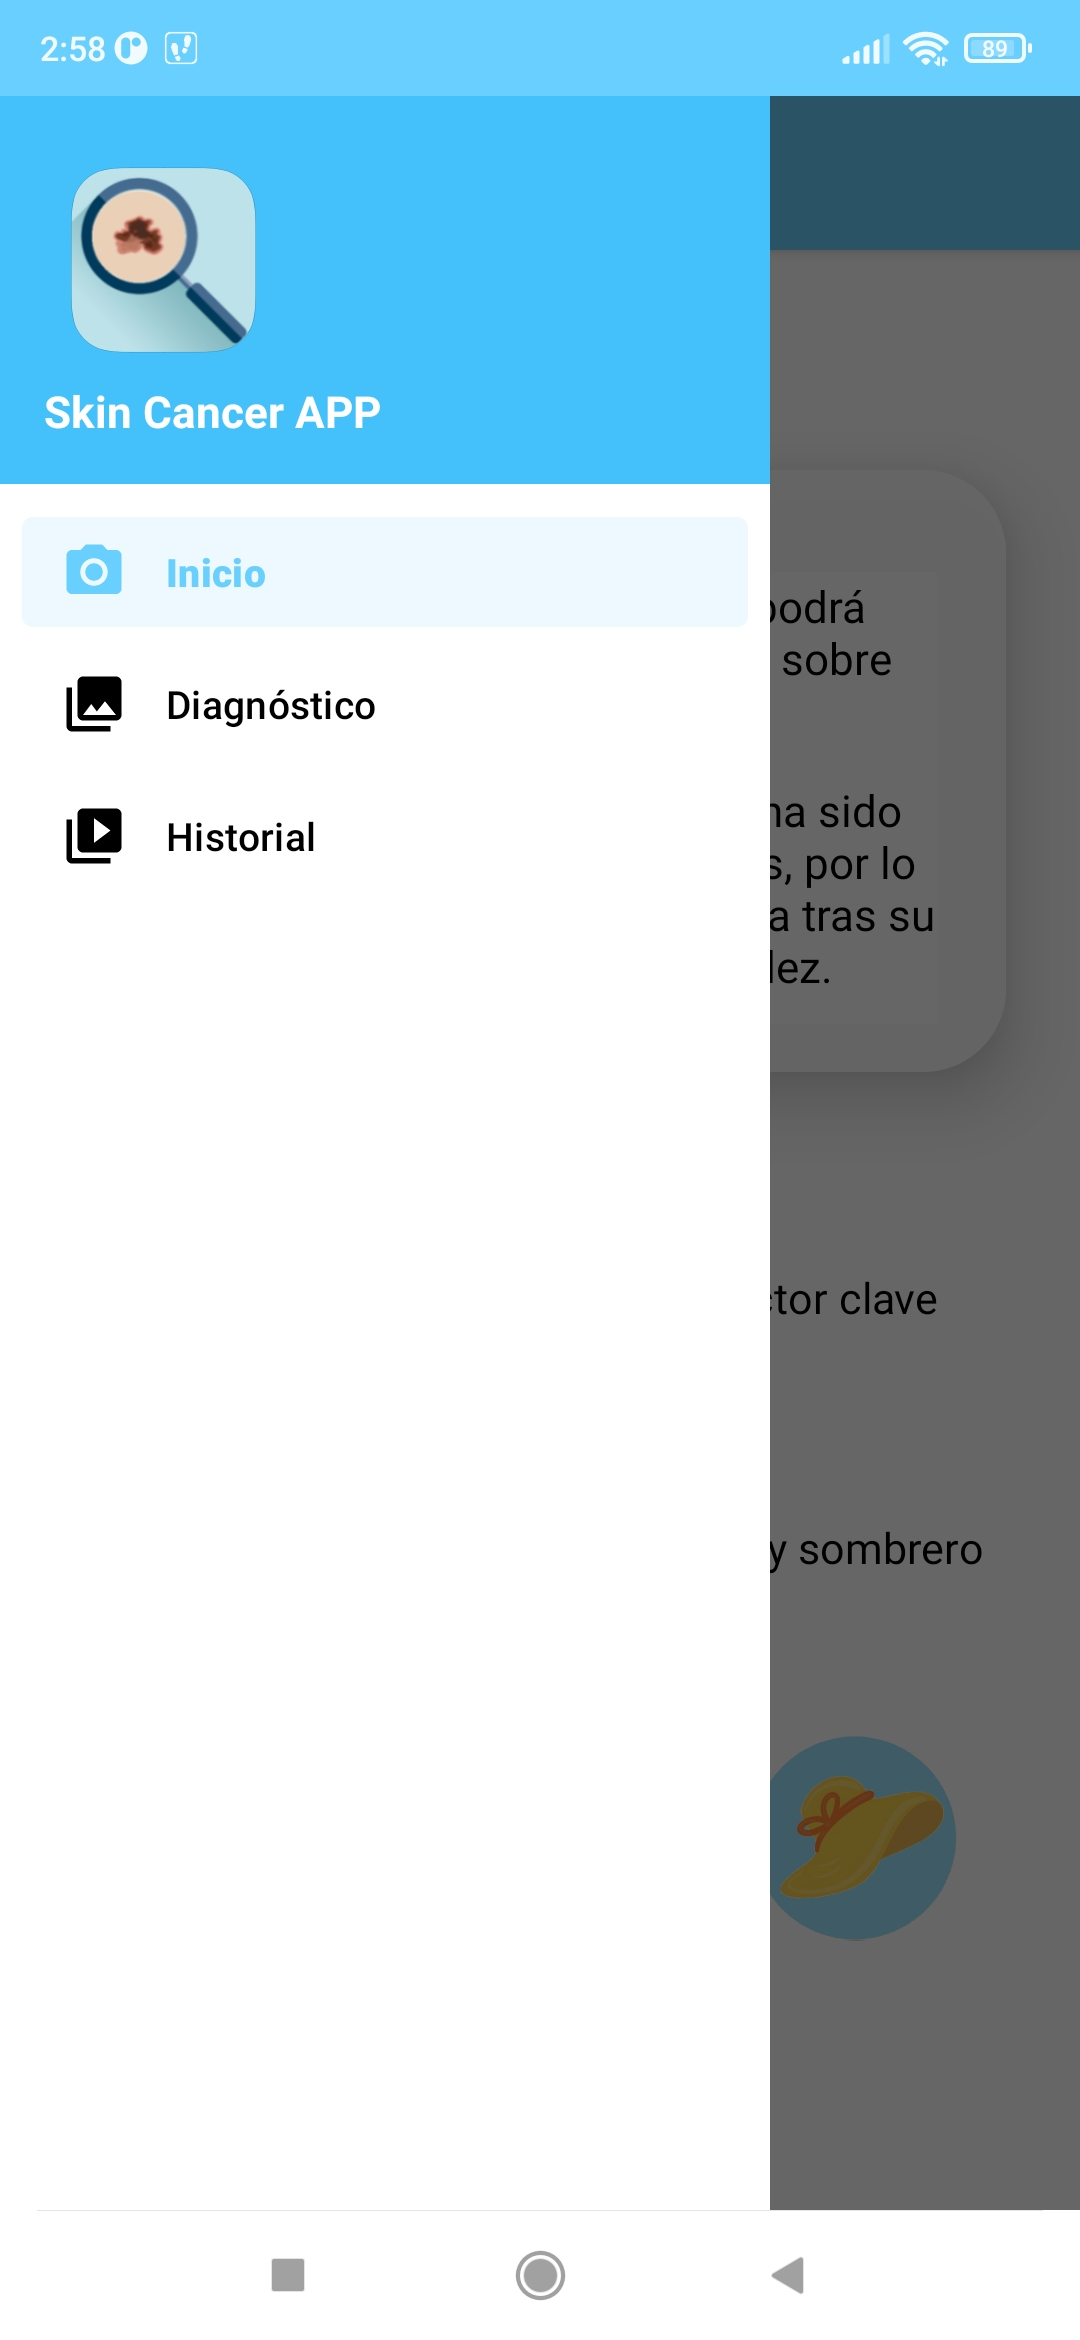
\includegraphics[scale = 0.125]{imagenes/menuapp.jpg}}
 	\caption{Interfaz de la aplicación: menús básicos}
 	\label{fig:inicioapp}
 \end{figure}
 
 \subsection{Realización de un diagnóstico}
 
 La realización de un diagnóstico es la funcionalidad elemental de la aplicación. Es la actividad que contiene la mayor carga computacional  de la misma, ya que se requiere realizar la carga de modelos y se procede posteriormente a la inferencia del resultado.
 
 El proceso, descrito a modo guion, engloba los siguientes pasos:
 \begin{enumerate}
 	\item \textbf{Seleccionar la ventana de diagnóstico}. Haciendo uso del menú lateral, el usuario debe dirigirse a la segunda opción, llamada  \textbf{Diagnóstico}, y representada con el icono de una fotografía (figura \ref{fig:inicioapp}).
 	\item \textbf{Seleccionar método de importación}. Dentro de la actividad de diagnóstico, la aplicación nos permite realizar la importación de imagen a diagnosticar mediante dos medios: el uso de la galería, y la toma de una fotografía mediante la cámara. Para iniciar el proceso de importación, se debe pulsar uno de dos grandes botones azules en la parte inferior de la ventana, según el origen de la imagen (ver en figura \ref{}).
 	\begin{enumerate}
 		\item Si selecciona tomar fotografía, se solicitarán permisos de acceso a ella, y podrá tomar una fotografía con la aplicación de cámara por defecto de su dispositivo.
 		\item Si selecciona abrir galería, de mostrará una solicitud de acceso a memoria, y a continuación, se muestra la galería en modo mosaico para seleccionar la imagen que se desee, como se aprecia en la figura \ref{fig:recortarapp}.
 	\end{enumerate}
 	\item \textbf{Recortado}. Tras la importación de la fotografía mediante alguno de los medios, se ofrece de forma opcional realizar el recorte de la misma. Este mecanismo es útil si la cámara no es capaz de enfocar debido a la cercanía, o la imagen es demasiado grande. Su funcionamiento se basa en desplazar las esferas que marcan las esquinas de la imagen para modificar el tamaño, y arrastrando desde el centro del rectángulo en caso de que se desee desplazar la región, como se puede apreciar en la figura \ref{fig:recortarapp}.
 	
 	\item \textbf {Comunicación del resultado}. Tras el recorte, se procede a realizar la clasificación de la imagen y a mostrar los resultados del diagnóstico de forma el usuario pueda comprender qué enfermedad sufre. Se muestran los campos enunciados a continuación y en la figura \ref{fig:diagnostico}.
 	\begin{itemize}
 		\item \textit{Bondad del resultado}. Especifica si se trata de una imagen benigna o maligna, y el porcentaje de seguridad del modelo. No representa una opinión médica real, sólo un valor indicativo procedente del modelo subyacente.
 		\item \textit{Tipo de enfermedad}. Tras la predicción binaria, se ha realizado también en segundo plano la clasificación mediante los modelos especializados, de forma que se muestran las tres enfermedades con mayor porcentaje de coincidencia dentro del conjunto benigno o maligno.
 		\item \textit{Descripción}. A título informativo, se muestra en pantalla una breve descripción acerca de la gravedad de la enfermedad, posibles orígenes y formas que posee.
 	\end{itemize}
 	
 	El usuario dispone de la posibilidad de desplazar hacia la izquierda el recuadro de la descripción para observar otras dos posibles clases que con un valor de probabilidad especificado pudieran tratarse de posibles alternativas (figura \ref{fig:diagnostico}).
 \end{enumerate}
 
    \begin{figure}[!ht]
 	\centering
 	\subfigure[Importación desde galería]{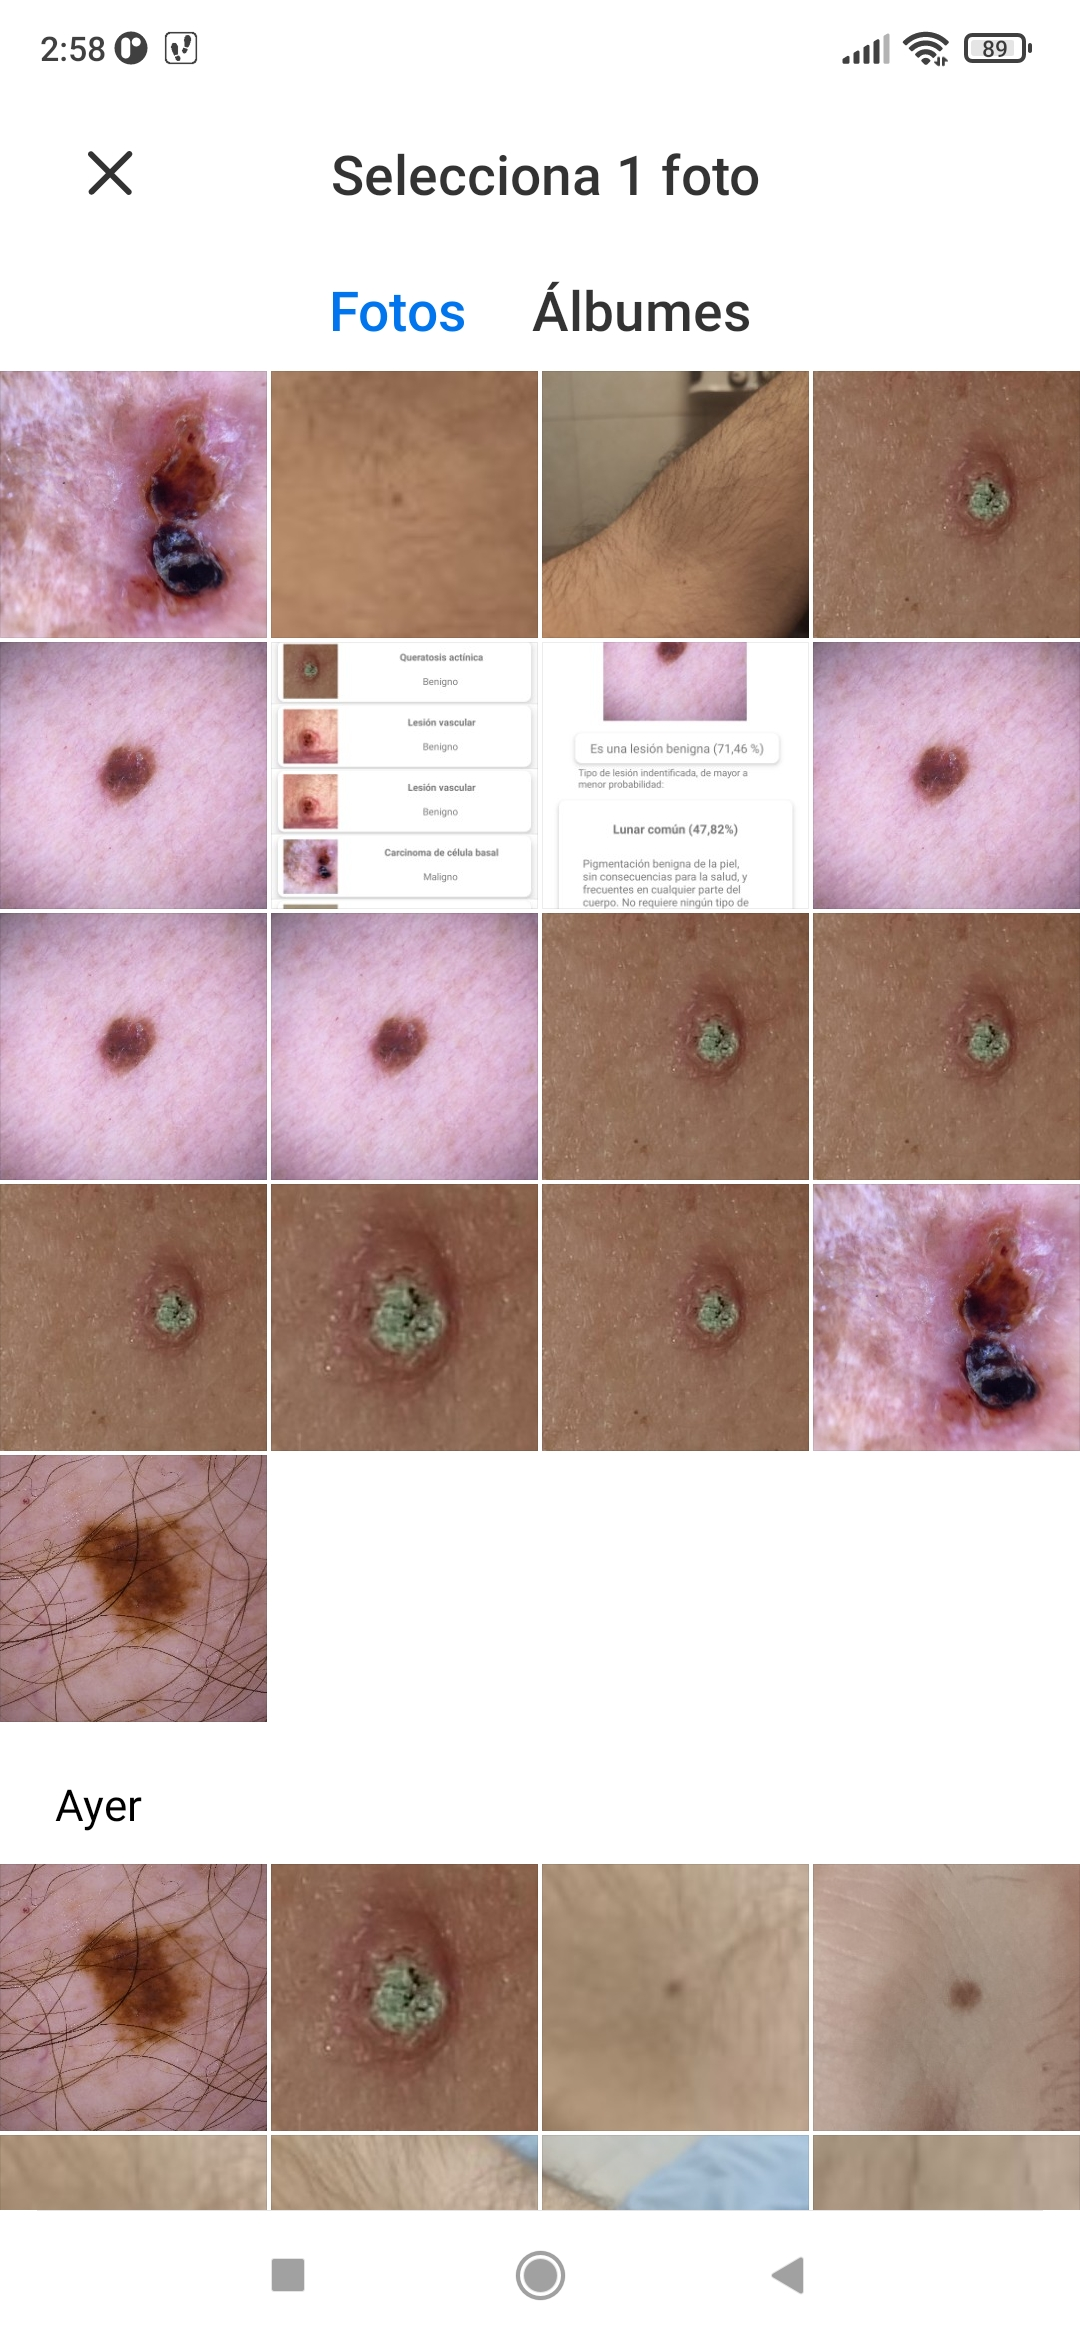
\includegraphics[scale = 0.125]{imagenes/galeriaapp.jpg}}
 	\subfigure[Recorte de la sección]{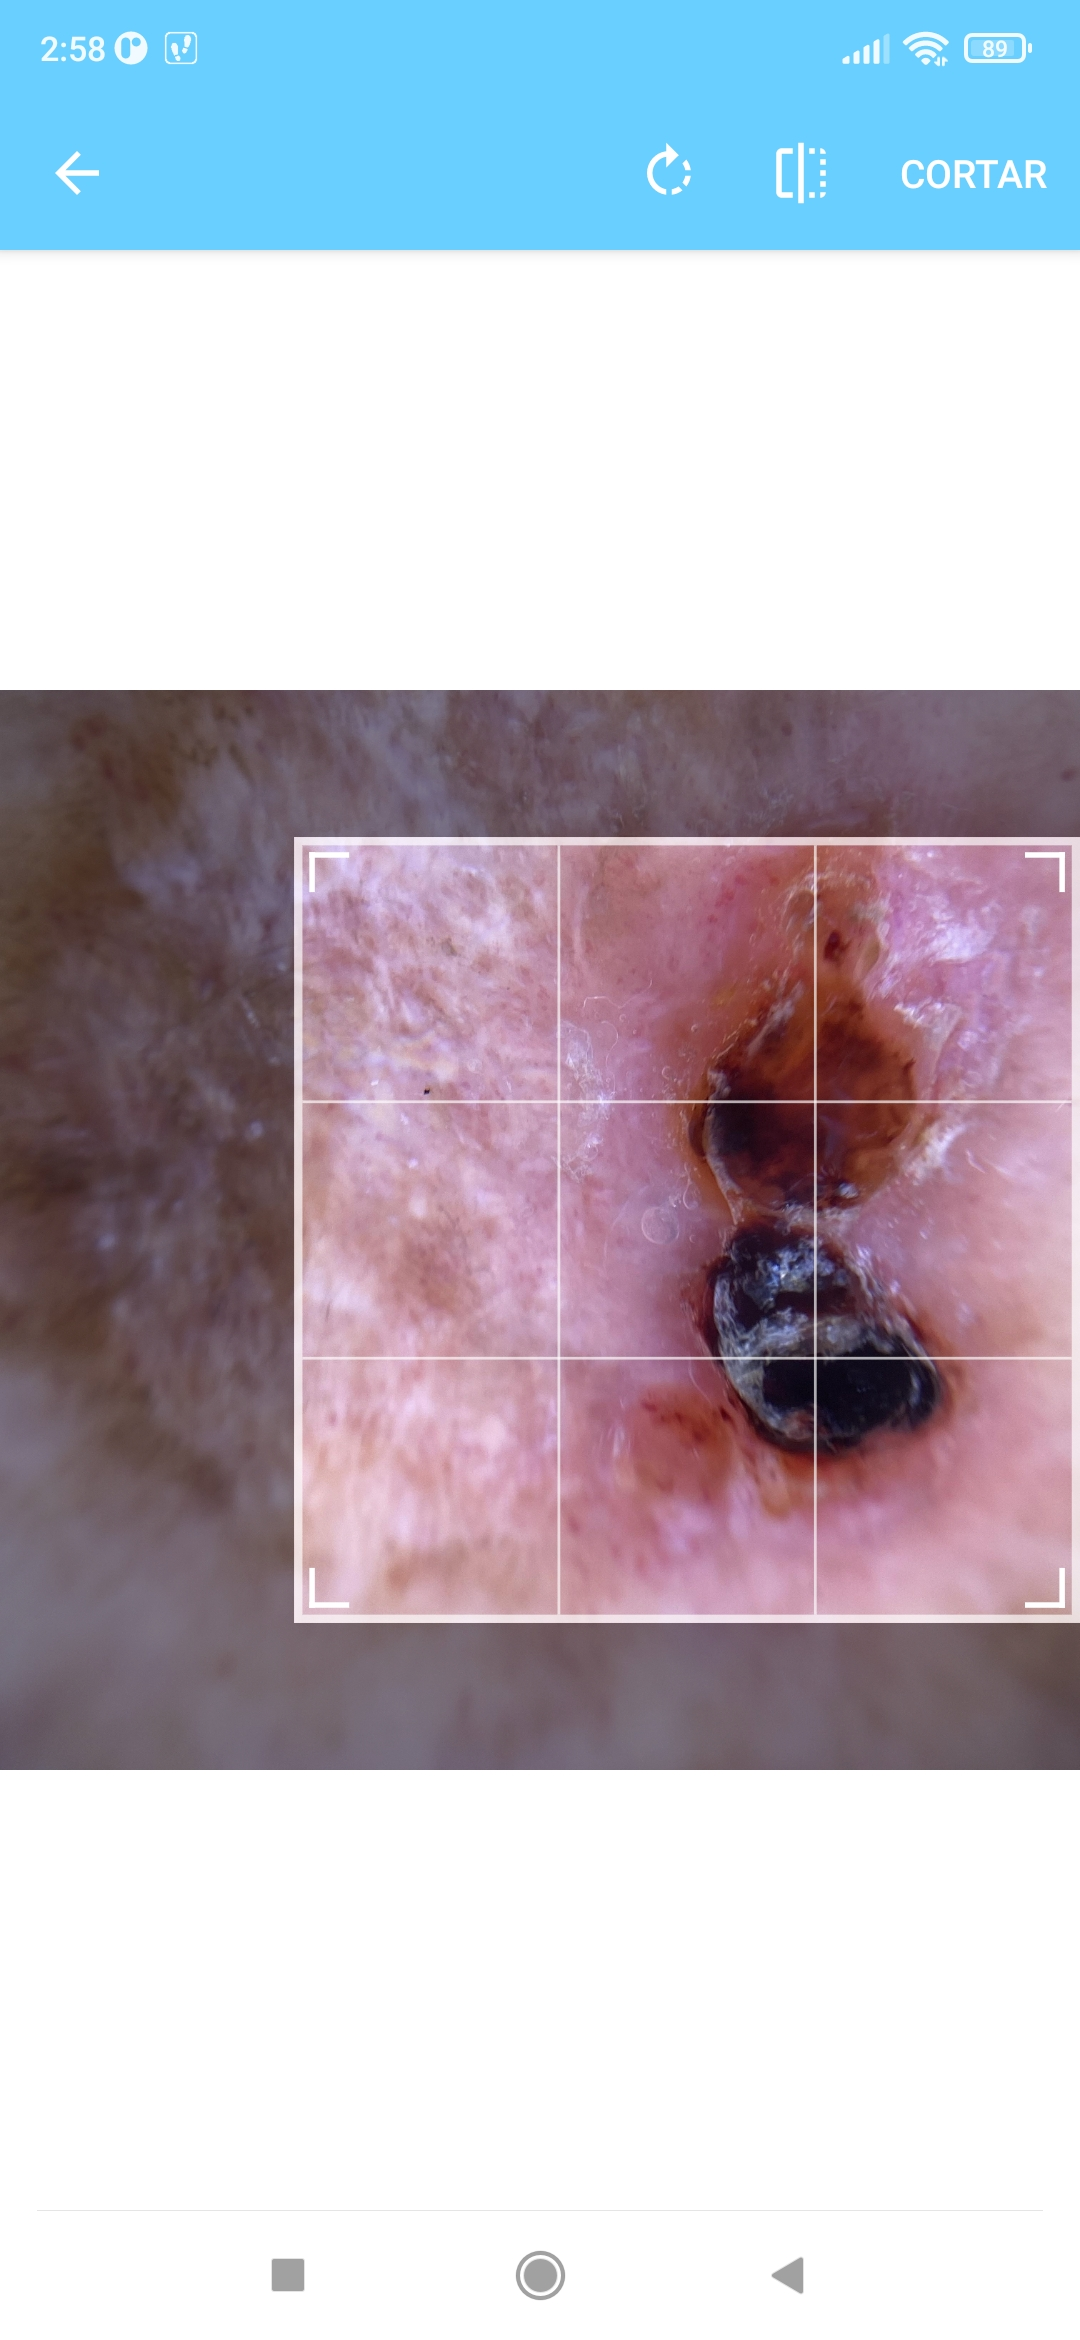
\includegraphics[scale = 0.125]{imagenes/recorteapp.jpg}}
 	\caption{Interfaz de la aplicación: selección desde galería y recorte de imágenes}
 	\label{fig:recortarapp}
 \end{figure}
 
     \begin{figure}[!ht]
 	\centering
 	\subfigure[Diagnóstico benigno (mediante cámara)]{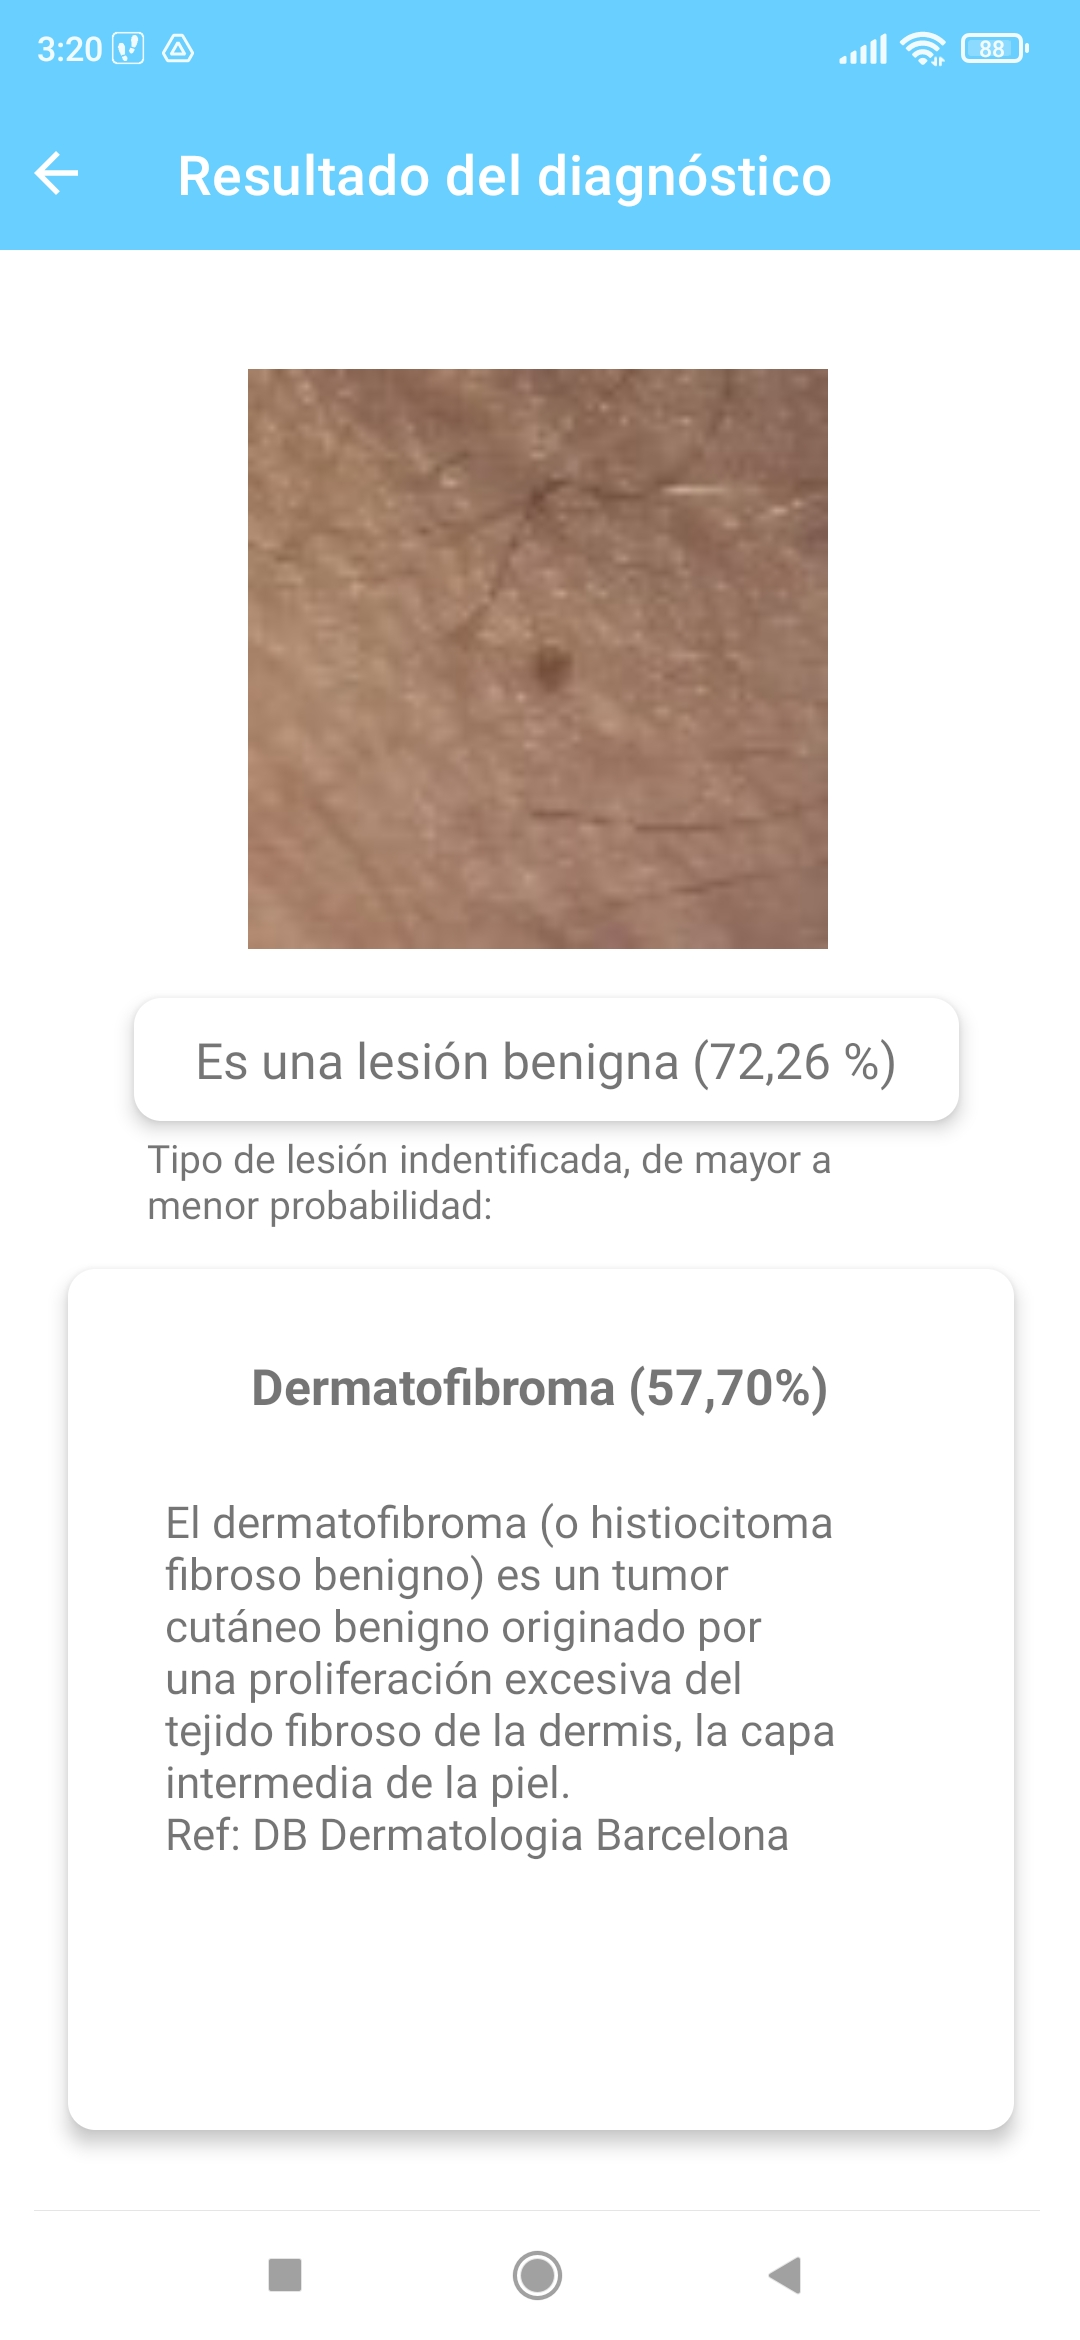
\includegraphics[scale = 0.125]{imagenes/diagnosticobenigno.jpg}}
 	\subfigure[Diagnóstico maligno (mediante galería)]{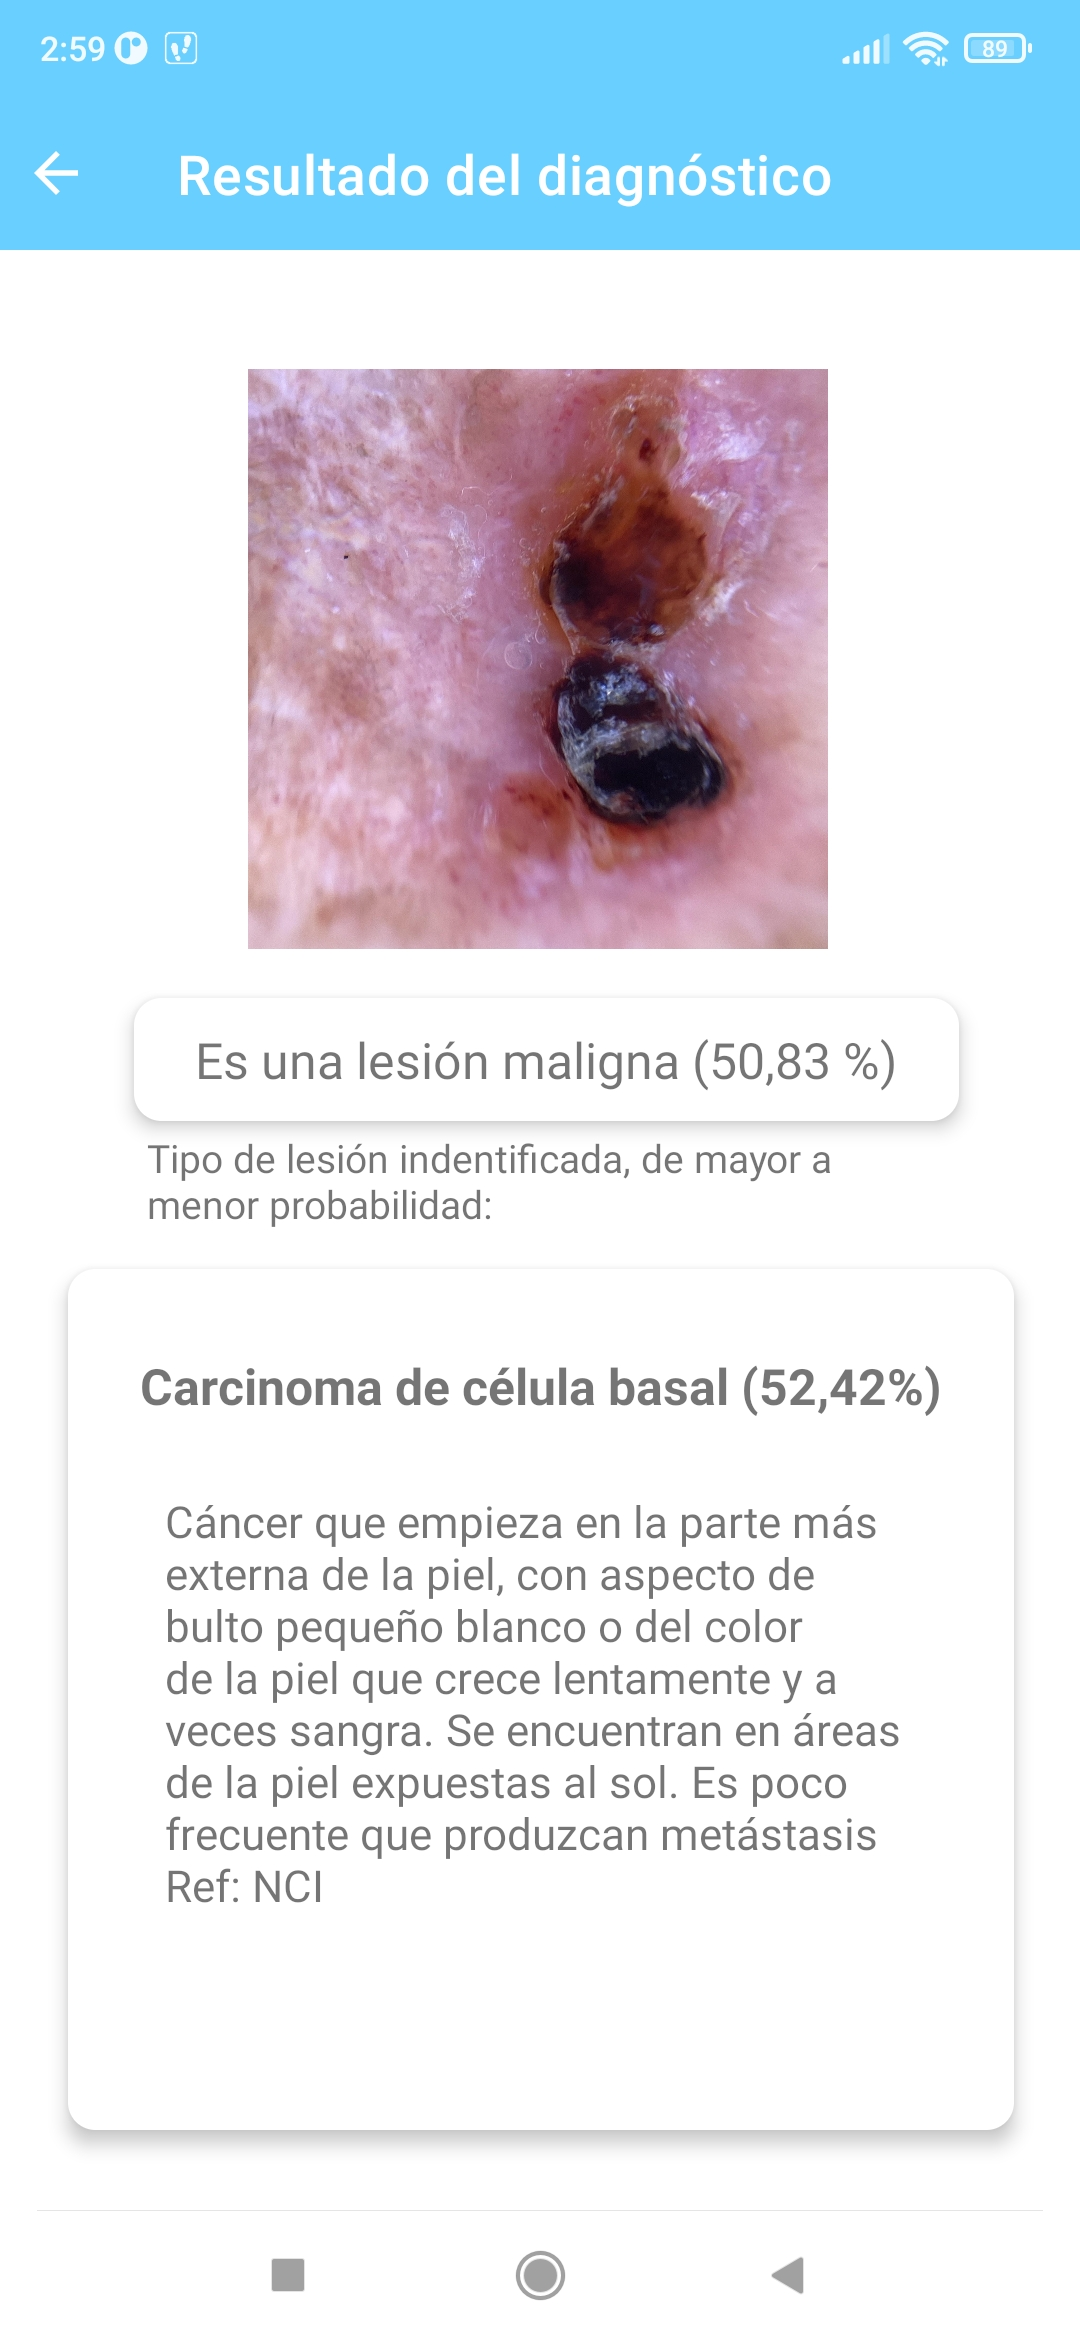
\includegraphics[scale = 0.125]{imagenes/diagnosticoapp.jpg}}
 	\caption{Interfaz de la aplicación: selección desde galería y recorte de imágenes}
 	\label{fig:diagnostico}
 \end{figure}
 
 
 \subsection{Consulta del historial}
 
 Todos los diagnósticos realizados por el usuario son almacenados en un fichero .json, el cual simula el comportamiento de una base de datos local. Son almacenadas en formato lista, de forma que si requiere comprobar la evolución de la enfermedad, sea capaz de comparar las imágenes y observar el diagnóstico ofrecido en aquel momento.  Para acceder a él, simplemente se deben seguir los pasos a continuación:
 
 \begin{enumerate}
 	\item \textbf{Seleccionar ventana de diagnóstico}. De la misma forma que la iniciación de la acción de diagnóstico, debemos seleccionar en el panel lateral el botón \textbf{Historial}, representado con un icono de elementos apilados.
 	\item \textbf{Búsqueda del diagnóstico}. Una vez accedido, es posible buscar el diagnóstico de interés gracias a su ordenado de mayor a menor cronología; es decir, los casos más antiguos aparecen primero, y los más recientes, últimos. La información proporcionada engloba:
 	\begin{enumerate}
 		\item \textit{Tipo de enfermedad}. Si el caso es maligno o benigno.
 		\item \textit{Diagnóstico}. Enfermedad específica con mayor valor de probabilidad.
 		\item \textit{Imagen}. Se crea la miniatura de la imagen durante el diagnóstico para ser mostrada en esta sección e identificar más fácilmente el caso a buscar. Adicionalmente, en caso de necesidad de comprobar la imagen completa, se guarda una copia de cada recorte realizado en la galería del dispositivo. Éstas podrían ser borradas, pero la miniatura permanecería en el historial.
 	\end{enumerate}
 \end{enumerate}
 
 En la figura \ref{fig:historial}, podemos observar un ejemplo de la distribución de los casos, los cuales se almacenan en formato de lista deslizable mediante scroll.
 
      \begin{figure}[H]
 	\centering
 	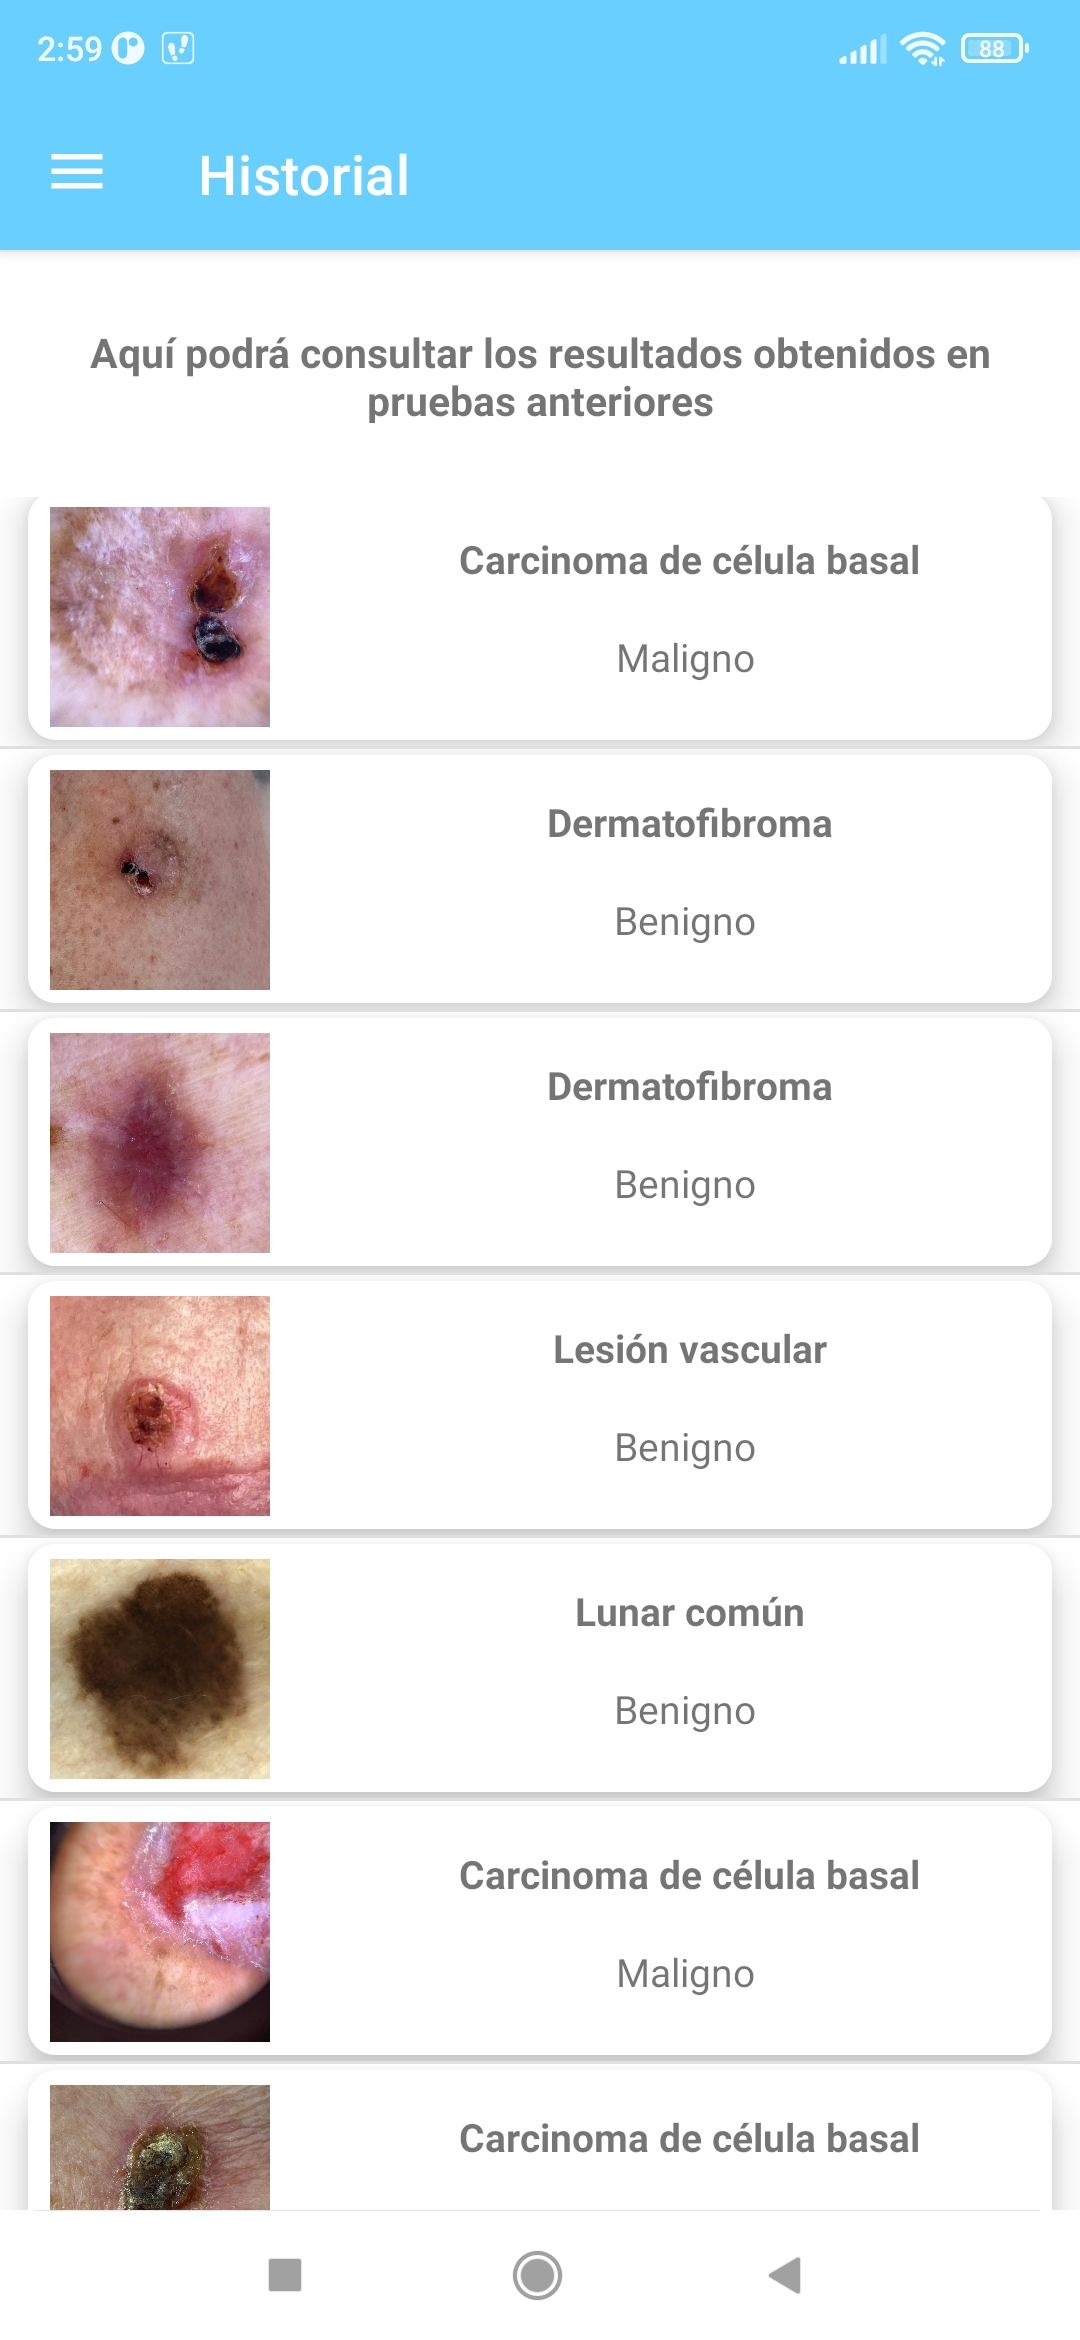
\includegraphics[scale = 0.125]{imagenes/historialapp.jpg}
 	\caption{Interfaz de la aplicación: historial}
 	\label{fig:historial}
 \end{figure}